%%%%%%%%%%%%%%%%%%%%%%%%%%%%%%%%%%%%%%%%%%
% The Legrand Orange Book
% LaTeX Template
% Version 2.0 (9/2/15)
%
% This template has been downloaded from:
% http://www.LaTeXTemplates.com
%
% Mathias Legrand (legrand.mathias@gmail.com) with modifications by:
% Vel (vel@latextemplates.com)
%
% License:
% CC BY-NC-SA 3.0 (http://creativecommons.org/licenses/by-nc-sa/3.0/)
%% Compiling this template:
% This template uses biber for its bibliography and makeindex for its index.
% When you first open the template, compile it from the command line with the 
% commands below to make sure your LaTeX distribution is configured correctly:
%
% 1) pdflatex main
% 2) makeindex main.idx -s StyleInd.ist
% 3) biber main
% 4) pdflatex main x 2
%
% After this, when you wish to update the bibliography/index use the appropriate
% command above and make sure to compile with pdflatex several times 
% afterwards to propagate your changes to the document.
%
% This template also uses a number of packages which may need to be
% updated to the newest versions for the template to compile. It is strongly
% recommended you update your LaTeX distribution if you have any
% compilation errors.
%
% Important note:
% Chapter heading images should have a 2:1 width:height ratio,
% e.g. 920px width and 460px height.
%
%%%%%%%%%%%%%%%%%%%%%%%%%%%%%%%%%%%%%%%%%

%----------------------------------------------------------------------------------------
%	PACKAGES AND OTHER DOCUMENT CONFIGURATIONS
%----------------------------------------------------------------------------------------

\documentclass[11pt,fleqn]{book} % Default font size and left-justified equations

%----------------------------------------------------------------------------------------

%%%%%%%%%%%%%%%%%%%%%%%%%%%%%%%%%%%%%%%%%
% The Legrand Orange Book
% Structural Definitions File
% Version 2.0 (9/2/15)
%
% Original author:
% Mathias Legrand (legrand.mathias@gmail.com) with modifications by:
% Vel (vel@latextemplates.com)
% 
% This file has been downloaded from:
% http://www.LaTeXTemplates.com
%
% License:
% CC BY-NC-SA 3.0 (http://creativecommons.org/licenses/by-nc-sa/3.0/)
%
%%%%%%%%%%%%%%%%%%%%%%%%%%%%%%%%%%%%%%%%%

%----------------------------------------------------------------------------------------
%	VARIOUS REQUIRED PACKAGES AND CONFIGURATIONS
%----------------------------------------------------------------------------------------

\usepackage[top=3cm,bottom=3cm,left=3cm,right=3cm,headsep=10pt,a4paper]{geometry} % Page margins

\usepackage{graphicx} % Required for including pictures
\graphicspath{{Pictures/}} % Specifies the directory where pictures are stored

\usepackage{lipsum} % Inserts dummy text

\usepackage{tikz} % Required for drawing custom shapes

\usepackage[english]{babel} % English language/hyphenation

\usepackage{enumitem} % Customize lists
\setlist{nolistsep} % Reduce spacing between bullet points and numbered lists

\usepackage{booktabs} % Required for nicer horizontal rules in tables

\usepackage{xcolor} % Required for specifying colors by name
\definecolor{ocre}{RGB}{243,102,25} % Define the orange color used for highlighting throughout the book
\usepackage{amsmath}
%----------------------------------------------------------------------------------------
%	FONTS
%----------------------------------------------------------------------------------------

\usepackage{avant} % Use the Avantgarde font for headings
%\usepackage{times} % Use the Times font for headings
\usepackage{mathptmx} % Use the Adobe Times Roman as the default text font together with math symbols from the Sym­bol, Chancery and Com­puter Modern fonts

\usepackage{microtype} % Slightly tweak font spacing for aesthetics
\usepackage[utf8]{inputenc} % Required for including letters with accents
\usepackage[T1]{fontenc} % Use 8-bit encoding that has 256 glyphs

%----------------------------------------------------------------------------------------
%	BIBLIOGRAPHY AND INDEX
%----------------------------------------------------------------------------------------

\usepackage[style=alphabetic,citestyle=numeric,sorting=nyt,sortcites=true,autopunct=true,babel=hyphen,hyperref=true,abbreviate=false,backref=true,backend=biber]{biblatex}
\addbibresource{bibliography.bib} % BibTeX bibliography file
\defbibheading{bibempty}{}

\usepackage{calc} % For simpler calculation - used for spacing the index letter headings correctly
\usepackage{makeidx} % Required to make an index
\makeindex % Tells LaTeX to create the files required for indexing

%----------------------------------------------------------------------------------------
%	MAIN TABLE OF CONTENTS
%----------------------------------------------------------------------------------------

\usepackage{titletoc} % Required for manipulating the table of contents

\contentsmargin{0cm} % Removes the default margin

% Part text styling
\titlecontents{part}[0cm]
{\addvspace{35pt}\centering\large\bfseries}
{}
{}
{}

% Chapter text styling
\titlecontents{chapter}[1.25cm] % Indentation
{\addvspace{12pt}\large\sffamily\bfseries} % Spacing and font options for chapters
{\color{ocre!60}\contentslabel[\Large\thecontentslabel]{1.25cm}\color{ocre}} % Chapter number
{\color{ocre}}  
{\color{ocre!60}\normalsize\;\titlerule*[.5pc]{.}\;\thecontentspage} % Page number

% Section text styling
\titlecontents{section}[1.25cm] % Indentation
{\addvspace{3pt}\sffamily\bfseries} % Spacing and font options for sections
{\contentslabel[\thecontentslabel]{1.25cm}} % Section number
{}
{\hfill\color{black}\thecontentspage} % Page number
[]

% Subsection text styling
\titlecontents{subsection}[1.25cm] % Indentation
{\addvspace{1pt}\sffamily\small} % Spacing and font options for subsections
{\contentslabel[\thecontentslabel]{1.25cm}} % Subsection number
{}
{\ \titlerule*[.5pc]{.}\;\thecontentspage} % Page number
[]

% List of figures
\titlecontents{figure}[0em]
{\addvspace{-5pt}\sffamily}
{\thecontentslabel\hspace*{1em}}
{}
{\ \titlerule*[.5pc]{.}\;\thecontentspage}
[]

% List of tables
\titlecontents{table}[0em]
{\addvspace{-5pt}\sffamily}
{\thecontentslabel\hspace*{1em}}
{}
{\ \titlerule*[.5pc]{.}\;\thecontentspage}
[]

%----------------------------------------------------------------------------------------
%	MINI TABLE OF CONTENTS IN PART HEADS
%----------------------------------------------------------------------------------------

% Chapter text styling
\titlecontents{lchapter}[0em] % Indenting
{\addvspace{15pt}\large\sffamily\bfseries} % Spacing and font options for chapters
{\color{ocre}\contentslabel[\Large\thecontentslabel]{1.25cm}\color{ocre}} % Chapter number
{}  
{\color{ocre}\normalsize\sffamily\bfseries\;\titlerule*[.5pc]{.}\;\thecontentspage} % Page number

% Section text styling
\titlecontents{lsection}[0em] % Indenting
{\sffamily\small} % Spacing and font options for sections
{\contentslabel[\thecontentslabel]{1.25cm}} % Section number
{}
{}

% Subsection text styling
\titlecontents{lsubsection}[.5em] % Indentation
{\normalfont\footnotesize\sffamily} % Font settings
{}
{}
{}

%----------------------------------------------------------------------------------------
%	PAGE HEADERS
%----------------------------------------------------------------------------------------

\usepackage{fancyhdr} % Required for header and footer configuration

\pagestyle{fancy}
\renewcommand{\chaptermark}[1]{\markboth{\sffamily\normalsize\bfseries\chaptername\ \thechapter.\ #1}{}} % Chapter text font settings
\renewcommand{\sectionmark}[1]{\markright{\sffamily\normalsize\thesection\hspace{5pt}#1}{}} % Section text font settings
\fancyhf{} \fancyhead[LE,RO]{\sffamily\normalsize\thepage} % Font setting for the page number in the header
\fancyhead[LO]{\rightmark} % Print the nearest section name on the left side of odd pages
\fancyhead[RE]{\leftmark} % Print the current chapter name on the right side of even pages
\renewcommand{\headrulewidth}{0.5pt} % Width of the rule under the header
\addtolength{\headheight}{2.5pt} % Increase the spacing around the header slightly
\renewcommand{\footrulewidth}{0pt} % Removes the rule in the footer
\fancypagestyle{plain}{\fancyhead{}\renewcommand{\headrulewidth}{0pt}} % Style for when a plain pagestyle is specified

% Removes the header from odd empty pages at the end of chapters
\makeatletter
\renewcommand{\cleardoublepage}{
\clearpage\ifodd\c@page\else
\hbox{}
\vspace*{\fill}
\thispagestyle{empty}
\newpage
\fi}

%----------------------------------------------------------------------------------------
%	THEOREM STYLES
%----------------------------------------------------------------------------------------

\usepackage{amsmath,amsfonts,amssymb,amsthm} % For math equations, theorems, symbols, etc

\newcommand{\intoo}[2]{\mathopen{]}#1\,;#2\mathclose{[}}
\newcommand{\ud}{\mathop{\mathrm{{}d}}\mathopen{}}
\newcommand{\intff}[2]{\mathopen{[}#1\,;#2\mathclose{]}}
\newtheorem{notation}{Notation}[chapter]

% Boxed/framed environments
\newtheoremstyle{ocrenumbox}% % Theorem style name
{0pt}% Space above
{0pt}% Space below
{\normalfont}% % Body font
{}% Indent amount
{\small\bf\sffamily\color{ocre}}% % Theorem head font
{\;}% Punctuation after theorem head
{0.25em}% Space after theorem head
{\small\sffamily\color{ocre}\thmname{#1}\nobreakspace\thmnumber{\@ifnotempty{#1}{}\@upn{#2}}% Theorem text (e.g. Theorem 2.1)
\thmnote{\nobreakspace\the\thm@notefont\sffamily\bfseries\color{black}---\nobreakspace#3.}} % Optional theorem note
\renewcommand{\qedsymbol}{$\blacksquare$}% Optional qed square

\newtheoremstyle{blacknumex}% Theorem style name
{5pt}% Space above
{5pt}% Space below
{\normalfont}% Body font
{} % Indent amount
{\small\bf\sffamily}% Theorem head font
{\;}% Punctuation after theorem head
{0.25em}% Space after theorem head
{\small\sffamily{\tiny\ensuremath{\blacksquare}}\nobreakspace\thmname{#1}\nobreakspace\thmnumber{\@ifnotempty{#1}{}\@upn{#2}}% Theorem text (e.g. Theorem 2.1)
\thmnote{\nobreakspace\the\thm@notefont\sffamily\bfseries---\nobreakspace#3.}}% Optional theorem note

\newtheoremstyle{blacknumbox} % Theorem style name
{0pt}% Space above
{0pt}% Space below
{\normalfont}% Body font
{}% Indent amount
{\small\bf\sffamily}% Theorem head font
{\;}% Punctuation after theorem head
{0.25em}% Space after theorem head
{\small\sffamily\thmname{#1}\nobreakspace\thmnumber{\@ifnotempty{#1}{}\@upn{#2}}% Theorem text (e.g. Theorem 2.1)
\thmnote{\nobreakspace\the\thm@notefont\sffamily\bfseries---\nobreakspace#3.}}% Optional theorem note

% Non-boxed/non-framed environments
\newtheoremstyle{ocrenum}% % Theorem style name
{5pt}% Space above
{5pt}% Space below
{\normalfont}% % Body font
{}% Indent amount
{\small\bf\sffamily\color{ocre}}% % Theorem head font
{\;}% Punctuation after theorem head
{0.25em}% Space after theorem head
{\small\sffamily\color{ocre}\thmname{#1}\nobreakspace\thmnumber{\@ifnotempty{#1}{}\@upn{#2}}% Theorem text (e.g. Theorem 2.1)
\thmnote{\nobreakspace\the\thm@notefont\sffamily\bfseries\color{black}---\nobreakspace#3.}} % Optional theorem note
\renewcommand{\qedsymbol}{$\blacksquare$}% Optional qed square
\makeatother

% Defines the theorem text style for each type of theorem to one of the three styles above
\newcounter{dummy} 
\numberwithin{dummy}{section}
\theoremstyle{ocrenumbox}
\newtheorem{theoremeT}[dummy]{Theorem}
\newtheorem{problem}{Problem}[chapter]
\newtheorem{exerciseT}{Exercise}[chapter]
\theoremstyle{blacknumex}
\newtheorem{exampleT}{Example}[chapter]
\theoremstyle{blacknumbox}
\newtheorem{vocabulary}{Vocabulary}[chapter]
\newtheorem{definitionT}{Definition}[section]
\newtheorem{corollaryT}[dummy]{Corollary}
\theoremstyle{ocrenum}
\newtheorem{proposition}[dummy]{Proposition}

%----------------------------------------------------------------------------------------
%	DEFINITION OF COLORED BOXES
%----------------------------------------------------------------------------------------

\RequirePackage[framemethod=default]{mdframed} % Required for creating the theorem, definition, exercise and corollary boxes

% Theorem box
\newmdenv[skipabove=7pt,
skipbelow=7pt,
backgroundcolor=black!5,
linecolor=ocre,
innerleftmargin=5pt,
innerrightmargin=5pt,
innertopmargin=5pt,
leftmargin=0cm,
rightmargin=0cm,
innerbottommargin=5pt]{tBox}

% Exercise box	  
\newmdenv[skipabove=7pt,
skipbelow=7pt,
rightline=false,
leftline=true,
topline=false,
bottomline=false,
backgroundcolor=ocre!10,
linecolor=ocre,
innerleftmargin=5pt,
innerrightmargin=5pt,
innertopmargin=5pt,
innerbottommargin=5pt,
leftmargin=0cm,
rightmargin=0cm,
linewidth=4pt]{eBox}	

% Definition box
\newmdenv[skipabove=7pt,
skipbelow=7pt,
rightline=false,
leftline=true,
topline=false,
bottomline=false,
linecolor=ocre,
innerleftmargin=5pt,
innerrightmargin=5pt,
innertopmargin=0pt,
leftmargin=0cm,
rightmargin=0cm,
linewidth=4pt,
innerbottommargin=0pt]{dBox}	

% Corollary box
\newmdenv[skipabove=7pt,
skipbelow=7pt,
rightline=false,
leftline=true,
topline=false,
bottomline=false,
linecolor=gray,
backgroundcolor=black!5,
innerleftmargin=5pt,
innerrightmargin=5pt,
innertopmargin=5pt,
leftmargin=0cm,
rightmargin=0cm,
linewidth=4pt,
innerbottommargin=5pt]{cBox}

% Creates an environment for each type of theorem and assigns it a theorem text style from the "Theorem Styles" section above and a colored box from above
\newenvironment{theorem}{\begin{tBox}\begin{theoremeT}}{\end{theoremeT}\end{tBox}}
\newenvironment{exercise}{\begin{eBox}\begin{exerciseT}}{\hfill{\color{ocre}\tiny\ensuremath{\blacksquare}}\end{exerciseT}\end{eBox}}				  
\newenvironment{definition}{\begin{dBox}\begin{definitionT}}{\end{definitionT}\end{dBox}}	
\newenvironment{example}{\begin{exampleT}}{\hfill{\tiny\ensuremath{\blacksquare}}\end{exampleT}}		
\newenvironment{corollary}{\begin{cBox}\begin{corollaryT}}{\end{corollaryT}\end{cBox}}	

%----------------------------------------------------------------------------------------
%	REMARK ENVIRONMENT
%----------------------------------------------------------------------------------------

\newenvironment{remark}{\par\vspace{10pt}\small % Vertical white space above the remark and smaller font size
\begin{list}{}{
\leftmargin=35pt % Indentation on the left
\rightmargin=25pt}\item\ignorespaces % Indentation on the right
\makebox[-2.5pt]{\begin{tikzpicture}[overlay]
\node[draw=ocre!60,line width=1pt,circle,fill=ocre!25,font=\sffamily\bfseries,inner sep=2pt,outer sep=0pt] at (-15pt,0pt){\textcolor{ocre}{R}};\end{tikzpicture}} % Orange R in a circle
\advance\baselineskip -1pt}{\end{list}\vskip5pt} % Tighter line spacing and white space after remark

%----------------------------------------------------------------------------------------
%	SECTION NUMBERING IN THE MARGIN
%----------------------------------------------------------------------------------------

\makeatletter
\renewcommand{\@seccntformat}[1]{\llap{\textcolor{ocre}{\csname the#1\endcsname}\hspace{1em}}}                    
\renewcommand{\section}{\@startsection{section}{1}{\z@}
{-4ex \@plus -1ex \@minus -.4ex}
{1ex \@plus.2ex }
{\normalfont\large\sffamily\bfseries}}
\renewcommand{\subsection}{\@startsection {subsection}{2}{\z@}
{-3ex \@plus -0.1ex \@minus -.4ex}
{0.5ex \@plus.2ex }
{\normalfont\sffamily\bfseries}}
\renewcommand{\subsubsection}{\@startsection {subsubsection}{3}{\z@}
{-2ex \@plus -0.1ex \@minus -.2ex}
{.2ex \@plus.2ex }
{\normalfont\small\sffamily\bfseries}}                        
\renewcommand\paragraph{\@startsection{paragraph}{4}{\z@}
{-2ex \@plus-.2ex \@minus .2ex}
{.1ex}
{\normalfont\small\sffamily\bfseries}}

%----------------------------------------------------------------------------------------
%	PART HEADINGS
%----------------------------------------------------------------------------------------

% numbered part in the table of contents
\newcommand{\@mypartnumtocformat}[2]{%
\setlength\fboxsep{0pt}%
\noindent\colorbox{ocre!20}{\strut\parbox[c][.7cm]{\ecart}{\color{ocre!70}\Large\sffamily\bfseries\centering#1}}\hskip\esp\colorbox{ocre!40}{\strut\parbox[c][.7cm]{\linewidth-\ecart-\esp}{\Large\sffamily\centering#2}}}%
%%%%%%%%%%%%%%%%%%%%%%%%%%%%%%%%%%
% unnumbered part in the table of contents
\newcommand{\@myparttocformat}[1]{%
\setlength\fboxsep{0pt}%
\noindent\colorbox{ocre!40}{\strut\parbox[c][.7cm]{\linewidth}{\Large\sffamily\centering#1}}}%
%%%%%%%%%%%%%%%%%%%%%%%%%%%%%%%%%%
\newlength\esp
\setlength\esp{4pt}
\newlength\ecart
\setlength\ecart{1.2cm-\esp}
\newcommand{\thepartimage}{}%
\newcommand{\partimage}[1]{\renewcommand{\thepartimage}{#1}}%
\def\@part[#1]#2{%
\ifnum \c@secnumdepth >-2\relax%
\refstepcounter{part}%
\addcontentsline{toc}{part}{\texorpdfstring{\protect\@mypartnumtocformat{\thepart}{#1}}{\partname~\thepart\ ---\ #1}}
\else%
\addcontentsline{toc}{part}{\texorpdfstring{\protect\@myparttocformat{#1}}{#1}}%
\fi%
\startcontents%
\markboth{}{}%
{\thispagestyle{empty}%
\begin{tikzpicture}[remember picture,overlay]%
\node at (current page.north west){\begin{tikzpicture}[remember picture,overlay]%	
\fill[ocre!20](0cm,0cm) rectangle (\paperwidth,-\paperheight);
\node[anchor=north] at (4cm,-3.25cm){\color{ocre!40}\fontsize{220}{100}\sffamily\bfseries\@Roman\c@part}; 
\node[anchor=south east] at (\paperwidth-1cm,-\paperheight+1cm){\parbox[t][][t]{8.5cm}{
\printcontents{l}{0}{\setcounter{tocdepth}{1}}%
}};
\node[anchor=north east] at (\paperwidth-1.5cm,-3.25cm){\parbox[t][][t]{15cm}{\strut\raggedleft\color{white}\fontsize{30}{30}\sffamily\bfseries#2}};
\end{tikzpicture}};
\end{tikzpicture}}%
\@endpart}
\def\@spart#1{%
\startcontents%
\phantomsection
{\thispagestyle{empty}%
\begin{tikzpicture}[remember picture,overlay]%
\node at (current page.north west){\begin{tikzpicture}[remember picture,overlay]%	
\fill[ocre!20](0cm,0cm) rectangle (\paperwidth,-\paperheight);
\node[anchor=north east] at (\paperwidth-1.5cm,-3.25cm){\parbox[t][][t]{15cm}{\strut\raggedleft\color{white}\fontsize{30}{30}\sffamily\bfseries#1}};
\end{tikzpicture}};
\end{tikzpicture}}
\addcontentsline{toc}{part}{\texorpdfstring{%
\setlength\fboxsep{0pt}%
\noindent\protect\colorbox{ocre!40}{\strut\protect\parbox[c][.7cm]{\linewidth}{\Large\sffamily\protect\centering #1\quad\mbox{}}}}{#1}}%
\@endpart}
\def\@endpart{\vfil\newpage
\if@twoside
\if@openright
\null
\thispagestyle{empty}%
\newpage
\fi
\fi
\if@tempswa
\twocolumn
\fi}

%----------------------------------------------------------------------------------------
%	CHAPTER HEADINGS
%----------------------------------------------------------------------------------------

\newcommand{\thechapterimage}{}%
\newcommand{\chapterimage}[1]{\renewcommand{\thechapterimage}{#1}}%
\def\@makechapterhead#1{%
{\parindent \z@ \raggedright \normalfont
\ifnum \c@secnumdepth >\m@ne
\if@mainmatter
\begin{tikzpicture}[remember picture,overlay]
\node at (current page.north west)
{\begin{tikzpicture}[remember picture,overlay]
\node[anchor=north west,inner sep=0pt] at (0,0) {\includegraphics[width=\paperwidth]{\thechapterimage}};
\draw[anchor=west] (\Gm@lmargin,-9cm) node [line width=2pt,rounded corners=15pt,draw=ocre,fill=white,fill opacity=0.5,inner sep=15pt]{\strut\makebox[22cm]{}};
\draw[anchor=west] (\Gm@lmargin+.3cm,-9cm) node {\huge\sffamily\bfseries\color{black}\thechapter. #1\strut};
\end{tikzpicture}};
\end{tikzpicture}
\else
\begin{tikzpicture}[remember picture,overlay]
\node at (current page.north west)
{\begin{tikzpicture}[remember picture,overlay]
\node[anchor=north west,inner sep=0pt] at (0,0) {\includegraphics[width=\paperwidth]{\thechapterimage}};
\draw[anchor=west] (\Gm@lmargin,-9cm) node [line width=2pt,rounded corners=15pt,draw=ocre,fill=white,fill opacity=0.5,inner sep=15pt]{\strut\makebox[22cm]{}};
\draw[anchor=west] (\Gm@lmargin+.3cm,-9cm) node {\huge\sffamily\bfseries\color{black}#1\strut};
\end{tikzpicture}};
\end{tikzpicture}
\fi\fi\par\vspace*{270\p@}}}

%-------------------------------------------

\def\@makeschapterhead#1{%
\begin{tikzpicture}[remember picture,overlay]
\node at (current page.north west)
{\begin{tikzpicture}[remember picture,overlay]
\node[anchor=north west,inner sep=0pt] at (0,0) {\includegraphics[width=\paperwidth]{\thechapterimage}};
\draw[anchor=west] (\Gm@lmargin,-9cm) node [line width=2pt,rounded corners=15pt,draw=ocre,fill=white,fill opacity=0.5,inner sep=15pt]{\strut\makebox[22cm]{}};
\draw[anchor=west] (\Gm@lmargin+.3cm,-9cm) node {\huge\sffamily\bfseries\color{black}#1\strut};
\end{tikzpicture}};
\end{tikzpicture}
\par\vspace*{270\p@}}
\makeatother

%----------------------------------------------------------------------------------------
%	HYPERLINKS IN THE DOCUMENTS
%----------------------------------------------------------------------------------------

\usepackage{hyperref}
\hypersetup{hidelinks,backref=true,pagebackref=true,hyperindex=true,colorlinks=false,breaklinks=true,urlcolor= ocre,bookmarks=true,bookmarksopen=false,pdftitle={Title},pdfauthor={Author}}
\usepackage{bookmark}
\bookmarksetup{
open,
numbered,
addtohook={%
\ifnum\bookmarkget{level}=0 % chapter
\bookmarksetup{bold}%
\fi
\ifnum\bookmarkget{level}=-1 % part
\bookmarksetup{color=ocre,bold}%
\fi
}
} % Insert the commands.tex file which contains the majority of the structure behind the template

\begin{document}

%----------------------------------------------------------------------------------------
%	TITLE PAGE
%----------------------------------------------------------------------------------------
%%


\begin{center}
        \par\nobreak
        {\color{ocre}\thickhrule}
        \vspace*{2cm}%
       \par\nobreak
    \makebox[0pt]{\Huge \bfseries  Elementary Experimental Higgs Physics }
        \vspace*{2cm}%
\par\nobreak
{\includegraphics[width=\linewidth,height=10cm]{Pictures/chapter_head_1.pdf}}
        \par\nobreak
 \vspace*{2cm}%
 \makebox[0pt]{\Huge \bfseries  HONR 268N} 
 \par\nobreak
        \vspace*{2cm}%
       {\color{ocre}\thickhrule}
  \end{center}
  
 
%\titleimage{chapter_head_1.pdf} % Table of contents heading image
%\title{Book Title}
\pagestyle{empty} % No headers

%\makebox[0pt][l]{%
%\raisebox{-\totalheight}[0pt][0pt]{%
%   {\transparent{0.4}\includegraphics[width=8in, height=11in]{chapter_head_1.pdf}}}}%%
%\BgThispage
 %Some content
%{\Huge\centering\bfseries\sffamily\parbox[c][][t]{\paperwidth}{\centering The Search for a Title\\[15pt] % Book title
%{\Large A Profound Subtitle}\\[20pt] % Subtitle
%{\huge Dr. John Smith}}}; % Author name

% \clearpage
% text

%\begingroup
%\thispagestyle{empty}
%\AddToShipoutPictureBG*
%\begin{tikzpicture}[remember picture,overlay]
%%%%sj\coordinate [below=12cm] (midpoint) at (current page.north);
%%%%sj\node at (current page.north west)
%%%%sj{\begin{tikzpicture}[remember picture,overlay]
%%%%sj\node[anchor=north west,inner sep=0pt] at (0,0) 
%{\includegraphics[width=\paperwidth, height=\paperwidth]{chapter_head_1.pdf}}; % Background image
%%%%sj\draw[anchor=north] (midpoint) node [fill=ocre!30!white,fill opacity=0.6,text opacity=1,inner sep=1cm]
%{\Huge\centering\bfseries\sffamily\parbox[c][][t]{\paperwidth}{\centering The Search for a Title\\[15pt] % Book title
%{\Large A Profound Subtitle}\\[20pt] % Subtitle
%{\huge Dr. John Smith}}}; % Author name
%%%%sj\end{tikzpicture}};
%%%%sj\end{tikzpicture}
%%%%sj\vfill
%\clearpage
%\endgroup

%----------------------------------------------------------------------------------------
%	COPYRIGHT PAGE
%----------------------------------------------------------------------------------------

%$$$#%\newpage
%$$$#%~\vfill
%$$$#%\thispagestyle{empty}

%$$$#%\noindent Copyright \copyright\ 2013 John Smith\\ % Copyright notice

%$$$#%\noindent \textsc{Published by Publisher}\\ % Publisher

%$$$#%\noindent \textsc{book-website.com}\\ % URL

%$$$#%\noindent Licensed under the Creative Commons Attribution-NonCommercial 3.0 Unported License (the ``License''). You may %$$$#%not use this file except in compliance with the License. You may obtain a copy of the License at %$$$#%\url{http://creativecommons.org/licenses/by-nc/3.0}. Unless required by applicable law or agreed to in writing, software %$$$#%distributed under the License is distributed on an \textsc{``as is'' basis, without warranties or conditions of any kind}, either %$$$#%express or implied. See the License for the specific language governing permissions and limitations under the License.\\ % %$$$#%License information

%$$$#%\noindent \textit{First printing, March 2013} % Printing/edition date

%----------------------------------------------------------------------------------------
%	TABLE OF CONTENTS
%----------------------------------------------------------------------------------------
\pagestyle{empty} % No headers
\vspace*{-10cm}%

\chapterimage{chapter_head_1.pdf} % Table of contents heading image
\tableofcontents  % Print the table of contents itself

 
\pagestyle{empty} % No headers
\vspace*{-10cm}%

%\cleardoublepage % Forces the first chapter to start on an odd page so it's on the right

\pagestyle{fancy} % Print headers again

%----------------------------------------------------------------------------------------
%	PART
%----------------------------------------------------------------------------------------

%$$$#%\part{Part One}

%----------------------------------------------------------------------------------------
%	CHAPTER 1
%----------------------------------------------------------------------------------------
\chapterimage{Pictures/chapter_head_2.pdf} % Chapter heading image
\chapter{Elementary Particles and Forces}

\section{Elementary Particles}\index{EP}
One of the questions that we, as human beings, have been asking since we started thinking, is “What is the universe made up of and what holds it together?" A long time ago, Democritus tried to answer the first part by defining “atoms” – although his definition of the atom was quite different from what we know about the atom today. In the last couple of centuries, we have come a long way in terms of answering the questions about the composition of matter and the glue that holds it together – giving us the form of the universe we see today.
The quest to answer the question “What is matter made of?” has been much like unraveling Russian nesting dolls. Everything, such as a chair, table, you, and me are made up of different kinds of molecules. Every molecule is made up of different kinds of atoms. All atoms, it turns out, even if they are different, have very similar structures – they all have one nucleus around which electrons revolve. The nucleus is made up of protons and neutrons. Protons are positively charged and electrons are negatively charged particles. The number of protons and electrons in a neutral atom are exactly equal so that the positive and negative charges cancel each other out.  All atoms are very similar in that they are all made up of protons, neutrons and electrons. However, a gold atom would be different from an iron atom or a hydrogen atom because they would have a different number of protons, neutrons and electrons.  




\begin{figure}[h]
\centering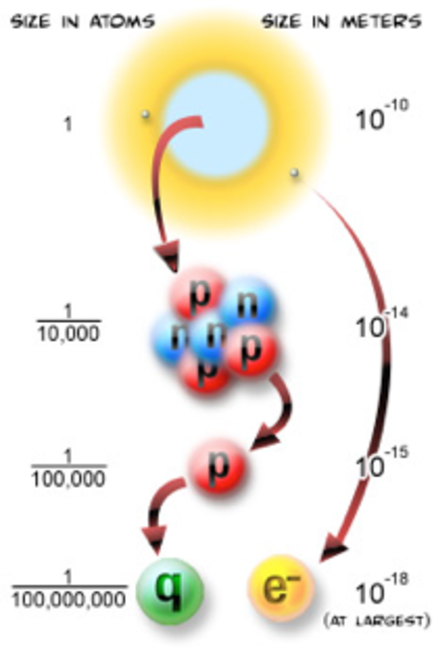
\includegraphics[scale=0.5]{./ElementaryParticles/Pictures/fi1.pdf}
\centering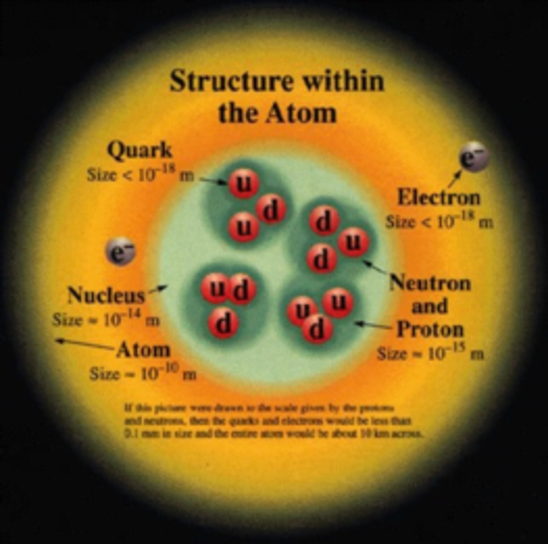
\includegraphics[scale=0.5]{./ElementaryParticles/Pictures/fig2.pdf}
\caption{The scale of fundamental particles}
\label{fig:fig1}
\end{figure}


However the atom is not the last of our Russian dolls. We know now that every proton and neutron itself is made up of even smaller particles, called quarks. Electrons, on the other hand, appear to be fundamental particles, that is, they cannot be further decomposed. 
So, as of now, we can divide fundamental particles into two categories - Quarks and Leptons.  There are 6 types of quarks and 6 types of leptons. Quite symmetric, don’t you think?  But the symmetry doesn’t end here. They seem to form 3 pairs (we call them families or generations) as you can see from Fig.2. 

Three generations of quarks (and leptons) are very similar in that they have same charge, spin etc. They differ in some internal quantum properties, but the most apparent difference is in mass – which increases as we go from 1st generation to 3rd.  As you can see from Table. 2 below, this difference is up to 5 orders of magnitude.

For every particle, there is also a corresponding anti particle.  Usually they have simple names, such as an anti-up quark or anti-neutrino.  The anti-particle for the electron, however, has the special name “positron”.  The existence of anti-matter was predicted when Paul Dirac unified quantum mechanics and Einstein’s theory of special relativity.  The anti-electron was discovered a few years later by Anderson.

\section{Forces} 
There are few other fundamental particles which don’t make up matter directly, but instead are exchanged in interactions between matter particles. These force carrier particles, when exchanged between two matter particles, make these particles interact through the force which they are carriers of. 

There are four known fundamental forces through which particles can interact and each has its own carrier particles. 

1.	Strong nuclear force 
Only quarks can feel this force through the exchange of force carrier particles called gluons. This force is much stronger compared to electromagnetic force of repulsion between the same charge protons and keeps the atomic nucleus stable.

2.	Weak nuclear force 
This is the force responsible for radioactive decay of atomic nuclei.  It has three force carrier particles W+, W-, and Z boson. It allows one type of quark to turn into another, usually within the same generation.  So a top quark can turn into a bottom quark by emitting a W boson.  It also allows charged leptons to change into a neutrino.  So a muon can decay to a muon neutrino by emitting a W boson.  The weak force is also very important in the fusion reactions that power the sun.

3.	Electromagnetic force
The force between charged particles is mediated through the exchange of electromagnetic force carrier particles called photons.  This is the same photon that makes up the light you see from sun or a bulb. This is the force of attraction (repulsion) between opposite (same) electric charges or magnetic poles. 

4.	Gravitational force
The everyday force that keeps us safely on the surface of the earth and is felt by all particles with mass. Graviton, the theorized particle proposed to be the force carrier for gravity has not been discovered yet. 

The forces and corresponding carrier particles are listed in Table.1.
Table 1: Fundamental forces and corresponding force carrier particles.

\section{Standard model of particle physics}
Going back to the question “what is the universe made up of and what holds it together?” our current understanding is that the matter in our visible universe is made up of quarks and leptons which interact with one another through force carrier particles.  There is a theory called the standard model of particle physics which describes this visible universe and, partly, the forces that hold it together. This theory, in principle, can describe all the physical process in chemistry and biology in terms of fundamental interactions The standard model of particle physics describes phenomenon concerning three out of the four known fundamental forces – electromagnetic force, weak force and strong force. The formal name for the mathematical structure of this theory is “gauge-invariant quantum field theory”.  Gauge-invariant means that the properties of the bosons (force mediators) are determined by symmetries relating the matter fields (quarks and leptons). 

The fundamental particles and some of their basic properties are listed in Table. 2.














Table 2: Fundamental particles and their properties.

\section{Properties of fundamental particles}
Every fundamental particle, for example a u quark, has exactly the same properties no matter where or how it is produced.   The quarks and leptons have similar properties like charge, mass, spin etc., but quarks have one extra property called color. Just like particles with electromagnetic charge can only interact through the electromagnetic force, only the particles with color charge can interact through the strong force. This color has nothing to do with the color of things we see, but is a quantum (or internal) property of these particles. Every quark comes in three colors – red, blue and green. This is a useful analogy because the particles we observe directly don’t seem to have this property. In other words, they are colorless. According to the quark theory, just like combining these three colors gives white, combining three quarks with these three quantum properties gives a particle which does not have any color. So every particle that we can directly observe should be made up of a combination of either three quarks or a quark and an anti-quark, giving us the color-less particles we observe. 

The charge of electrons and protons is equal but opposite. We say electrons and protons have 1 unit of charge (-1e for an electron and +1e for a proton, where e is the charge of an electron). When quark theory was formulated, the charge of a proton equaling +1e had to be accounted for. In order to make sure that proton’s charge comes out to be equal to +1e, the constituent quarks were given fractional charges, as shown in Table. 2.

The everyday matter (atoms) is made up of protons, neutrons and electrons. The proton is made of two u quarks and one d quark (does the sum of their charges work?), Thus, in terms of fundamental particles,  everyday matter is made up of u and d quarks and the electron.  These particles belong to the first family of quarks and leptons. One of the big questions physicists are trying to answer is “Why do we need three families of particles?” The standard model also does not describe phenomenon concerning force of gravity. The recent cosmological discoveries of dark matter and dark energy are also open questions not addressed by this theory. 

Let’s count: 

Fermions: There are 6 leptons - electron, muon, tau and the corresponding three neutrinos.
There are 6 quarks - up, down, charm, strange, top and bottom. Every quark comes in 3 colors.
Leptons and quarks are both fermions, as they all have half integer spin 1/2.

Now multiply the total number of particles by 2 – all these particles have their anti-particles. For every quark, there is an anti-quark, and for every lepton there is an anti-lepton. These anti-particles are almost identical to their corresponding particles except for a very few properties.  For example, an electron’s anti-particle has the same mass but a positive charge (called positron).

Bosons: There are force carriers corresponding to four forces – photon, W+,W-,  Z and gluons.  These are all bosons with integer spin 1.

By 1995, all of the particles predicted by the standard model were discovered except one – the Higgs boson with spin 0. In 2012, a new boson was discovered at the Large Hadron Collider.  The studies done so far seem to indicate that this newly observed particle is very similar to the Higgs boson predicted by the standard model. 

\section{Non-Fundamental (composite) particles}
Apart from fundamental particles, more than 200 subatomic particles (made up of known fundamental particles) have been discovered using particle accelerators and detectors (see http://pdg.lbl.gov for a listing of the known particles).  These composite particles are made up of quarks, and are of two types:
Baryons: are made of three quarks, for example neutron and proton.
Mesons: are made of quark pairs for example pions.
Baryons and mesons are collectively called Hadrons.
Quantum Mechanics and Particle Physics
One generally only attempts to learn about particle physics after studying quantum mechanics.  Quantum mechanics is indeed fundamental to particle physics.  However, if a student’s goal is to become involved in particle physics research, it is only strictly necessary to learn a small fraction of this fascinating subject.  In this section, we will try to describe the minimum amount of quantum mechanics you need to understand particle physics.  To really learn quantum mechanics, you need first to study differential equations, and many of your class mates are just not there yet.
Quantum mechanics is strongly relate to one of the fundamental constants of nature, called h or h-bar (  ) where  .    has the numeric value of 1.054x10-34 Js.  If you see this constant in an equation, you know quantum mechanics is involved.
Often quantum mechanical systems involve quantization of energies.  The classic example is the energy states of the hydrogen atom (or any atom or molecule).  The electrons can only have certain energies.  If an atom absorbs energy, it can only do this if the energy is the right amount to move the electron between one of these discrete states (approximately… there are corrections to this that are important only when being very precise).  Likewise when an atom that is in one of the higher energy states “de-excites”, it can only emit photons with energies
For example, photons, the fundamental “packet” of electromagnetic radiation, can only have energies that are integer multiples of the product of its angular frequency (  where f is the frequency of the photon’s oscillation and   where c is the speed of light and   is the photon’s wavelength) and .  Thus   where n is an integer.
When you combine this with the energy levels of atoms, you get the characteristic absorption/emission spectra of atoms/molecules which can be used to identify them.
 
Figure 3: figure stolen from facultu.admiramar.edu
Another important thing to know about quantum mechanics is that it is probabilistic, in the sense often for a given initial state (say, an electron aimed at a piece of metal) there may be many possible final states (say, amount of energy that the electron loses, and the deflection of the electron from its initial direction).  In quantum mechanics, you can only calculate the probabilities of the different possible outcomes; you cannot ever, even with perfect information about the initial state, predict exactly what the final state will be.
Finally, there is the Heisenberg uncertainty principal.  


\section{The world's shortest description of quantum mechanics}

One generally only attempts to learn about particle physics after studying quantum mechanics.  Quantum mechanics is indeed fundamental to particle physics.  However, if a student’s goal is to become involved in particle physics research, it is only strictly necessary to learn a small fraction of this fascinating subject.  In this section, we will try to describe the minimum amount of quantum mechanics you need to understand particle physics.  To really learn quantum mechanics, you need first to study differential equations, and many of your class mates are just not there yet.
Quantum mechanics is strongly relate to one of the fundamental constants of nature, called h or h-bar (  ) where  .    has the numeric value of 1.054x10-34 Js.  If you see this constant in an equation, you know quantum mechanics is involved.
Often quantum mechanical systems involve quantization of energies.  The classic example is the energy states of the hydrogen atom (or any atom or molecule).  The electrons can only have certain energies.  If an atom absorbs energy, it can only do this if the energy is the right amount to move the electron between one of these discrete states (approximately… there are corrections to this that are important only when being very precise).  Likewise when an atom that is in one of the higher energy states “de-excites”, it can only emit photons with energies
For example, photons, the fundamental “packet” of electromagnetic radiation, can only have energies that are integer multiples of the product of its angular frequency (  where f is the frequency of the photon’s oscillation and   where c is the speed of light and   is the photon’s wavelength) and .  Thus   where n is an integer.
When you combine this with the energy levels of atoms, you get the characteristic absorption/emission spectra of atoms/molecules which can be used to identify them.


\begin{figure}[h]
\centering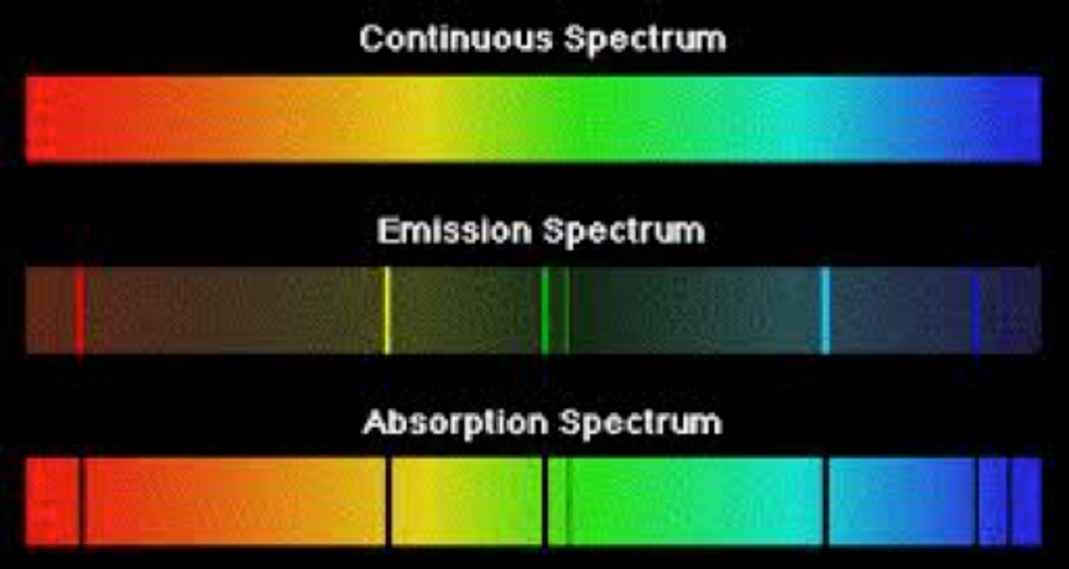
\includegraphics[scale=0.5]{./ElementaryParticles/Pictures/fig6.pdf}
\caption{absorption and emission lines}
\label{fig:light}
\end{figure}


Another important thing to know about quantum mechanics is that it is probabilistic, in the sense often for a given initial state (say, an electron aimed at a piece of metal) there may be many possible final states (say, amount of energy that the electron loses, and the deflection of the electron from its initial direction).  In quantum mechanics, you can only calculate the probabilities of the different possible outcomes; you cannot ever, even with perfect information about the initial state, predict exactly what the final state will be.
Finally, there is the Heisenberg uncertainty principal.  



\section{Feynman Diagrams}

Feynman diagrams began as a mnemonic to help particle theorists do the very complicated calculations required by gauge-invariant quantum field theories.  These calculations are done using something which is very important to practicing physicists, but rarely mentioned in undergraduate curriculum: perturbation theory.  In perturbation theory, you first calculate an approximate answer (the “leading order” calculation or LO).  You then calculation a correction to this answer (the “next to leading order” calculation or NLO).  You then calculate a correction to this correction (NNLO).  The Feynman diagrams represent aids to help in each order of the calculation.  However, they are also useful for just helping to visualize how bosons are exchanged between quarks/leptons to create interactions.

Figure~\ref{fig:fig8} below shows the “LO” diagram for annihilation of an up quark and an anti-up quark to a Z boson to an electron-positron pair.


\begin{figure}[h]
\centering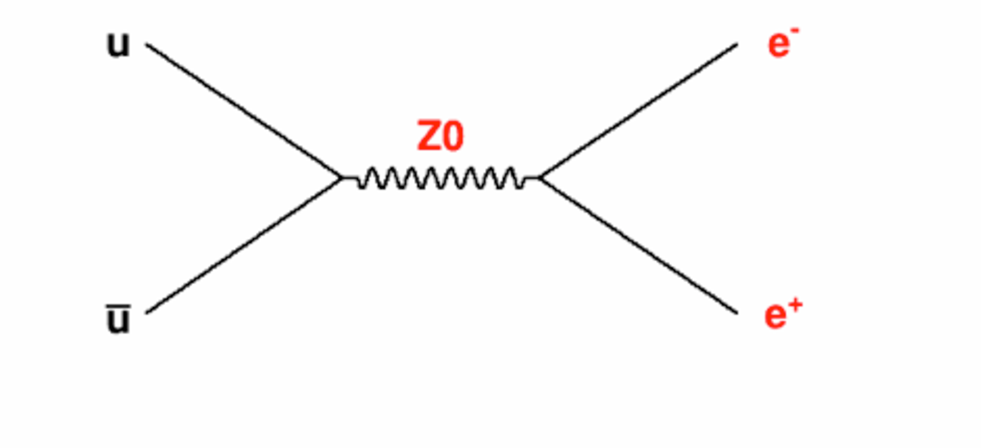
\includegraphics[scale=0.5]{./ElementaryParticles/Pictures/fig8.pdf}
\caption{LO Feynmann diagram for production of an electron position pair via a Z boson through the annihilation of an up and anti-up}
\label{fig:fig8}
\end{figure}
 

Figure ~\ref{fig:fig9} shows a NNLO (in the strong force) diagram for the same process.
 
\begin{figure}[h]
\centering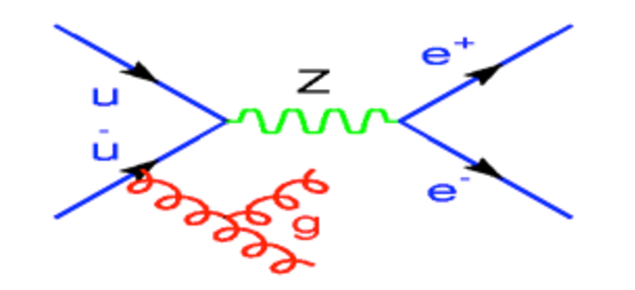
\includegraphics[scale=0.5]{./ElementaryParticles/Pictures/fig9.pdf}
\caption{NLO Feynmann diagram for production of an electron position pair via a Z boson through the annihilation of an up and anti-up}
\label{fig:fig9}
\end{figure}


\section{More on Mesons}
Mesons are bound states of 2 quarks.  These are very important for particle physics because, although the proton is the lightest stable particle, mesons are the lightest states containing quarks.  They are “unstable”, meaning that they decay, sometimes very quickly, to other types of particles.
The lightest mesons are called pions.  There are three of them, one with a positive charge, one neutral, and one with a negative charge.  The charged pions decay via the weak force to a muon and a neutrino.  The neutral pion usually decays to two photons.
The naming conventions for all the mesons are very strange because the standard model and the existence of quarks was not yet understood when they were discovered.  Thus there are “kaons” that contain strange quarks, “D mesons” that contain charm quarks.

As with the hydrogen atoms, there are also excited state of the two bound quarks.  While with hydrogen, we just say “excited hydrogen”, with the mesons, the excited states often have separate names, as it was not understood at the time of their discovery that they were essentially “excited pions”.  Thus rho mesons, eta mesons, etc are in a sense excited states of bound states of the up and down quark.

\section{The Higgs}
The  Higgs  boson  plays  a  special  role  in  the  standard  model.    Gauge
-
invariant  quantum  field  theories 
generally 
predict  that  the  force  bosons  should  be  massless.    And  indeed  the  photon  (E\&M),  the  gluon 
(strong force) are massless.  Although gravity can not yet be described by quantum field theory, in general a 
$1/r^2$ force indicates a massless boson, and gravity does
seem to follow this prescription.   Thus naively the 
standard model predicts that the W and Z boson should be massless.  However, instead, they have a mass 
about 100x that of the proton!  
The resolution was the Higgs.


\section{Further reading}
\begin{itemize}
\item pdg.lbl.gov is always a great site for all things related to particle physics
\item “Modern Particle Physics” by Mark Thomson
\item “Introduction to Elementary Particle Physics” by Alessandro Bettini
\end{itemize}




%----------------------------------------------------------------------------------------
%	CHAPTER 2
%----------------------------------------------------------------------------------------
\chapterimage{Pictures/chapter_head_2.pdf} % Chapter heading image
\chapter{Special Relativity}
 \section{Disclaimer}\index{Disclaimer}

Einstein's theory of special relativity is one of the most fascinating, elegant, surprising, and powerful theories in modern physics.  The derivation of its laws, beginning from the simple postulate that the speed of light is a constant, independent of the velocity of the person measuring it, along with the resulting profound implications in electromagnetic theory and the nature of space and time is astounding. We, unfortunately, do not have the time to cover everything in this course.  And you, as freshmen, for the most part are just not ready.  You will study this theory in depth when you take 300-level E\&M.

However, to understand what is going on at the LHC, you do need to understand some relativity.  The goal of this tutorial is to teach you the minimum needed to understand the Higgs discovery.  We will approach it from a practical point of view. Although this is anathema to the physicist in you, we will give you formulas without telling you where they come from.  You need to just accept them (For now! Until you are older!) as experimental reality, just as you accept $\vec{F}=m\vec{a}$  as a fact that you can use as a tool to work other problems.

\section{4-vectors}\index{4-vectors}

When doing Newtonian mechanics, you are taught about vectors.  You typically work with vectors that have three components, associated with three spatial directions (x, y, z).  Often, you then parameterize these components as a function of a time.  You might calculate the height of a particle above the ground (z) as a function of time, its z-component of velocity as a function of time, or its momentum as a function of time.

With special relativity, instead of these 3-vectors, we will work with 4 component vectors (4-vectors).  The fourth component for our position vector will be {\it time}.  However, time and position have different units (seconds for time and meters distance).  Mixing time and distance is thus mixing apples and oranges, so what can be done?

In special relativity, the speed of light is very special.  It is a constant, and all observers, regardless of their relative velocity, will get the same result when they measure it. We will discuss this more later.  Since this is a special number, one of the {\it fundamental constants} of nature, along with  $\hbar$ the fundamental constant of quantum physics, and a few other fundamental numbers.  We can use c to convert time to a distance and write our 4 vector for {\it event} (something that has a time and a position) as
\begin{equation}
	  {\color{red} d}=(ct,x,y,z)
\end{equation}

\noindent Every 3-vector will be augmented this way, although the associated {\it time-like component} may not be obvious to you at this stage.  Most importantly, momentum becomes 4-momentum, defined as
\begin{equation}  
{\color{red} p}=(E,cp_x, cp_y, cp_z)  
\end{equation}

where E is the particle's energy. Again, we use c to make sure all components have the same units.
	 
We will use red to denote 4 vectors and the usual vector notation to denote 3 vectors.  Thus we can write:
\begin{equation} 
\textcolor{red}{p}=(E,cp_x, cp_y, cp_z)  
\end{equation}  		   
\begin{equation} 
{\color{red} p}=(E,c\vec{p})  
\end{equation} 
\vspace{.2cm} 
\begin{minipage}{0.9\textwidth} 
\begin{framed}
%\vspace{.1cm}
\begin{exercise}
%\begin{frshaded}
%\fcolorbox{\bordercolor}{\backgroundcolor} 
{show that E and cp have the same units. Remember that the $i^{th}$ component of force is related to energy by $F_i=\frac{dE}{dx_i}$
 and to momentum by $F_i = \frac{dp_i}{dt}$}
\end{exercise}
%\end{frshaded}
%\vspace{.1cm}
\end{framed} 
\end{minipage}
\vspace{.2cm}



As you may remember from your high school physics, there are several important mathematical operations that are used with vectors.  One is the dot product, a way of making a scalar out of two vectors.  You may remember that:
\begin{equation}
      C= \vec A \cdot \vec B = A_xB_x +A_yB_y +A_zB_z 
\end{equation}
The dot product of a vector with itself gives the square of the magnitude of the vector.
\begin{equation}      
     |{\vec{A}|^2} =\vec A \cdot \vec A  
\end{equation}	  
\noindent The dot product, in Newtonian physics, is used in calculating work from force and displacement.

There is a dot-like product associated with 4 vectors, and it has some very interesting, useful, and sometimes bewildering properties.
\begin{equation}
	    c ={\color{red}a} \cdot {\color{red}b} = a_0b_0 - \vec a \cdot \vec b
\end{equation}
More on this useful operation later.

\section{Frames (center-of-mass, lab) and transforming between frames}\index{Frames (center-of-mass, lab) and transforming between frames}

Imagine two people, (A and B) with rulers and stop watches.  A is standing in the sidewalk on Route One, while B is in a white car in the left hand lane going south on Route One.  Both see a red car in the right hand lane going south which passes the car containing B.  However, person A sees the space between her and red car increasing at a much faster rate than person B sees the space between him and the red car increasing.  They each measure a different velocity for the red car relative to themselves.  Mathematically, what we have in 1 spatial dimension; it is easy to extend to 3 spatial dimensions.

\noindent let $v_B, x_B$ be the velocity and relative to person A 
       
\noindent let $v_{RA}, x_{RA},v_{RB}, x_{RB}$
	  

Then,
\begin{equation}
 v_{RB} = v_{RA} - v_B
\end{equation}
\begin{equation}
 x_{RB} = x_{RA} - v_B t
\end{equation}

\noindent This set of equations that transform a variable as it is measured in one frame to the value it will have when measured in another frame is called {\it Galilean Relativity}.


However, in relativity, if the red car were moving at the speed of light both A and B would see the distance between them and the car increasing at the same rate.  In other words, all observers will measure the same speed of light regardless of their relative velocities.  Obviously, the equations given above do not predict this.  Einstein developed new equations that give us a measurement in one frame relative to another.  


\begin{equation} ct_{RB} = \gamma(ct_{RA} - \beta x_{RA}) \end{equation} 
\begin{equation}  x_{RB} = \gamma(- \beta ct_{RA} + x_{RA}) 	 \end{equation} 

\noindent where,

\begin{equation} \beta = v_B /c \end{equation}   	
\begin{equation} \gamma = \frac{1}{\sqrt{1- \beta^2}} \end{equation}  


Note that $\beta$  is a number between 0 and 1, and is the fraction of the speed of light the other measured frame has with respect to your frame of reference.  $\gamma$  is a number that is greater than 1.  It is called the {\it relativistic boost} and will be very useful.

In general, any 4-vector will transform this way.  Thus, the {\color{red} energy-momentum 4-vector will transform in this way}.  This set of transformation equations is called {\it Special Relativity} or the {\it Lorentz transformation}.

Note that these are extremely weird equations.  They imply that observers that are not at rest with respect to each other will not agree on the time when something occurred. They will not agree if two things happening at two different positions happened at the same time or not.  There are lots of fascinating implications to this, but you will just have to take more advanced physics to learn about them.  We are going to concentrate on the minimum you need to look for new particles at the LHC.

\section{Length of 4 vectors}\index{Length of 4 vectors}

A 4 vector has the interesting property that all observers, regardless of their relative velocities, will agree on: the length of a 4-vector.
Let's prove this in one spatial dimension (I think you can do the
equivalent proof in 3-D using this model!). 

Lengths of 4 vectors
\begin{eqnarray}
|a|^2 &=&  a_0 a_0 - a_x a_x  \nonumber \\
      &=&  |a'|^2 = a'_0 a'_0 - a'_x a'_x  \nonumber \\
      &=& \gamma (a_0 -\beta a_x) \gamma (a_0 -\beta a_x) - \gamma (-\beta a_0 +a_x ) \gamma (-\beta a_0 +a_x )  \nonumber \\
      &=&  \gamma^2 (a_0^2  -2 \beta a_x a_0  + \beta^2 a_x^2 - \beta^2 a_0^2  + 2 a_x \beta  a_0  - a_x^2)   \nonumber \\
      &=& =\gamma^2 ( a_0^2 (1-  \beta^2)  - a_x^2 (1-  \beta^2))   \nonumber \\
      &=&  a_0^2 - a_x^2  \nonumber  \\
      &=& |a|^2  
\end{eqnarray} 

In particular, this is true for the energy-momentum 4 vector  $|{\color{red}p}|^2 = E^2 - (pc)^2$  . (working in 1 spatial dimension! you can extend this to 3)  In fact, 
\begin{equation}
	  	(mc^2)^2 = E^2 -(pc)^2
\end{equation}  
In the rest frame of a particle (the frame where  $|\vec p |$  is zero), you get the famous equation that appears on T-shirts everywhere.

This equation is very important to the LHC.  When we look for particles, we recognize them by their mass.  W bosons have a mass of 80 GeV.  Z bosons have a mass of 91 GeV.  Top quarks have a mass of 173 GeV.  Obviously, we cannot put particles on a scale to weigh them. This equation tells us that, if we want to see the mass of a particle made in a collision, we just need to know its energy and momentum.  Then, from that, we can determine its mass.  We can also show that it doesn't matter what our velocity is with respect to the particle.  This equation will always give us the mass of that particle, and that all observers will agree on the mass.

\section{Momentum and Energy}\index{relE}
Once you are at high enough speeds that you need to take relativity into account, the old formulas for momentum ($p=mv$) and kinetic energy ($E=1/2 mv^2$) no longer work.

You must instead use:
$$
E=\gamma m
$$

$$
KE=(\gamma -1) m
$$

and

$$
p=\beta E
$$


\section{HEP units}\index{HEP units}

Masses in GeV?  What kind of mass unit is that? You may be more used to kg or g or lbs.  Remember that the eV is a unit of energy, defined as the potential energy gained when an electron moves from one position to another whose potential is higher by 1 V.

We know from Einstein that mass is related to energy through $c^2$.  So $eV/c^2$ is a unit of mass.  GeV/$c^2$ is then $10^6$ eV/$c^2$.  For scale, the proton has a mass of 1 GeV/$c^2$.

Particle physicists are lazy.  They hate to type even a single extra letter.  Particle physicists are lazier than most.  They have defined a whole unit system designed to help them avoid typing $c$ and $\hbar$ .  Unit systems need a way of defining a time unit, a distance unit, and a weight unit.  

$c$ is related to both the time and distance unit.  The units of  $\hbar$ are Energy x time. We know from Einstein that energy is related to mass, so we can use it instead of mass as our third necessary unit.  The eV, which is the potential energy an electron gains when it transverses a potential difference of 1 V, is chosen to be the unit of energy. Length and time units are then chosen so that both $c$ and $\hbar$  are 1.  

Once we do that, GeV/$c^2$ just becomes GeV/$1^2$ or GeV. Not only that, but we can also measure both length and time in GeV.

\noindent For example  $\hbar$/GeV is a unit of time.  But $\hbar$ =1 in this unit system, so GeV$^{-1}$ is a unit of time.  c/GeV is a unit of length.  So GeV$^{-1}$ is also a unit of length.


In this unit system, the length of the energy-momentum 4-vector becomes (in 1 dimension):
\begin{equation}
	  m^2 = E^2 - p^2
\end{equation}  	 


\section{Lifetimes of particles}

An interesting consequence of special relativity is that the lifetime you measure for a particle will depend on its velocity relative to you.  Let $\tau _0$  be the lifetime you measure for the particle when the particle is at rest with respect to you.  Then, using equation 1.4, we can see that the lifetime for a particle moving with a velocity $\beta$  is
\begin{equation}
	 \tau  = \gamma \tau _0
\end{equation}  	 

\noindent The lifetime is longer for a moving particle than it is for one at rest by a factor $\gamma$.

\section{Breit-Wigner}

We have learned that most heavy particles are not stable, and decay.  Above, we said that particles are identified by their mass, and that particles have a well-defined mass characteristic of their type.  However, this is not quite true.  As you will learn when you take quantum mechanics, a quantum state cannot have a well defined time and a well defined energy (mass).  This is expressed through the Heisenberg uncertainty principle:
\begin{equation}
	 \Delta E \Delta t   \ge \hbar
\end{equation} 

\noindent Because of this, when we measure the particle's mass, we get a range of values.  How big is that range?  Remember that we can express the lifetime of a particle, using our new funny units, in GeV, using:
 \begin{equation}
	 \Gamma =   \frac{\hbar}{\tau _0}
\end{equation} 
	  

\noindent where  $\Gamma$ is the lifetime in GeV.  When the lifetime is expressed in GeV,  it is referred to as the particle's width.

\noindent The actual functional form of the mass distribution is called a Breit-Wigner.  The form is:

\begin{equation} \text{rate  of  events} \propto \frac{1}{(E-M)^2 + \frac{\Gamma}{2}} \end{equation} 

\noindent where M is the value of the peak of the mass distribution and E is the observed mass.

\vspace{.2cm} 
\begin{minipage}{0.9\textwidth} 
\begin{framed}
%\vspace{.1cm}
\begin{exercise}
%\begin{frshaded}
%\fcolorbox{\bordercolor}{\backgroundcolor} 
{For the Z boson, M is 91.2 GeV and $\Gamma$  is 2.5 GeV.  What is the corresponding lifetime?  Use root to plot this function versus E, the observed mass.}
\end{exercise}
%\end{frshaded}
%\vspace{.1cm}
\end{framed} 
\end{minipage}
\vspace{.2cm}



\section{The coordinate system for a collider experiment}

The CMS detector, whose data we will be using in this course, uses a right-handed coordinate system, with the origin at the nominal interaction point, the x axis pointed to the center of the LHC, the y axis pointing up (perpendicular to the LHC plane), and the z axis along the anticlockwise-beam direction.  The polar angle   is measured from the positive z axis and the azimuthal angle  $\phi$  is measured in the x-y plane.

\section{Collisions (conservation of 4-momentum)}

When two protons appear to collide in a detector, what really collides is the {\it partons} (either quarks or gluons) inside the protons.  A sketch of a collision that produces a Z boson is shown below.
 

\begin{figure}[h]
\centering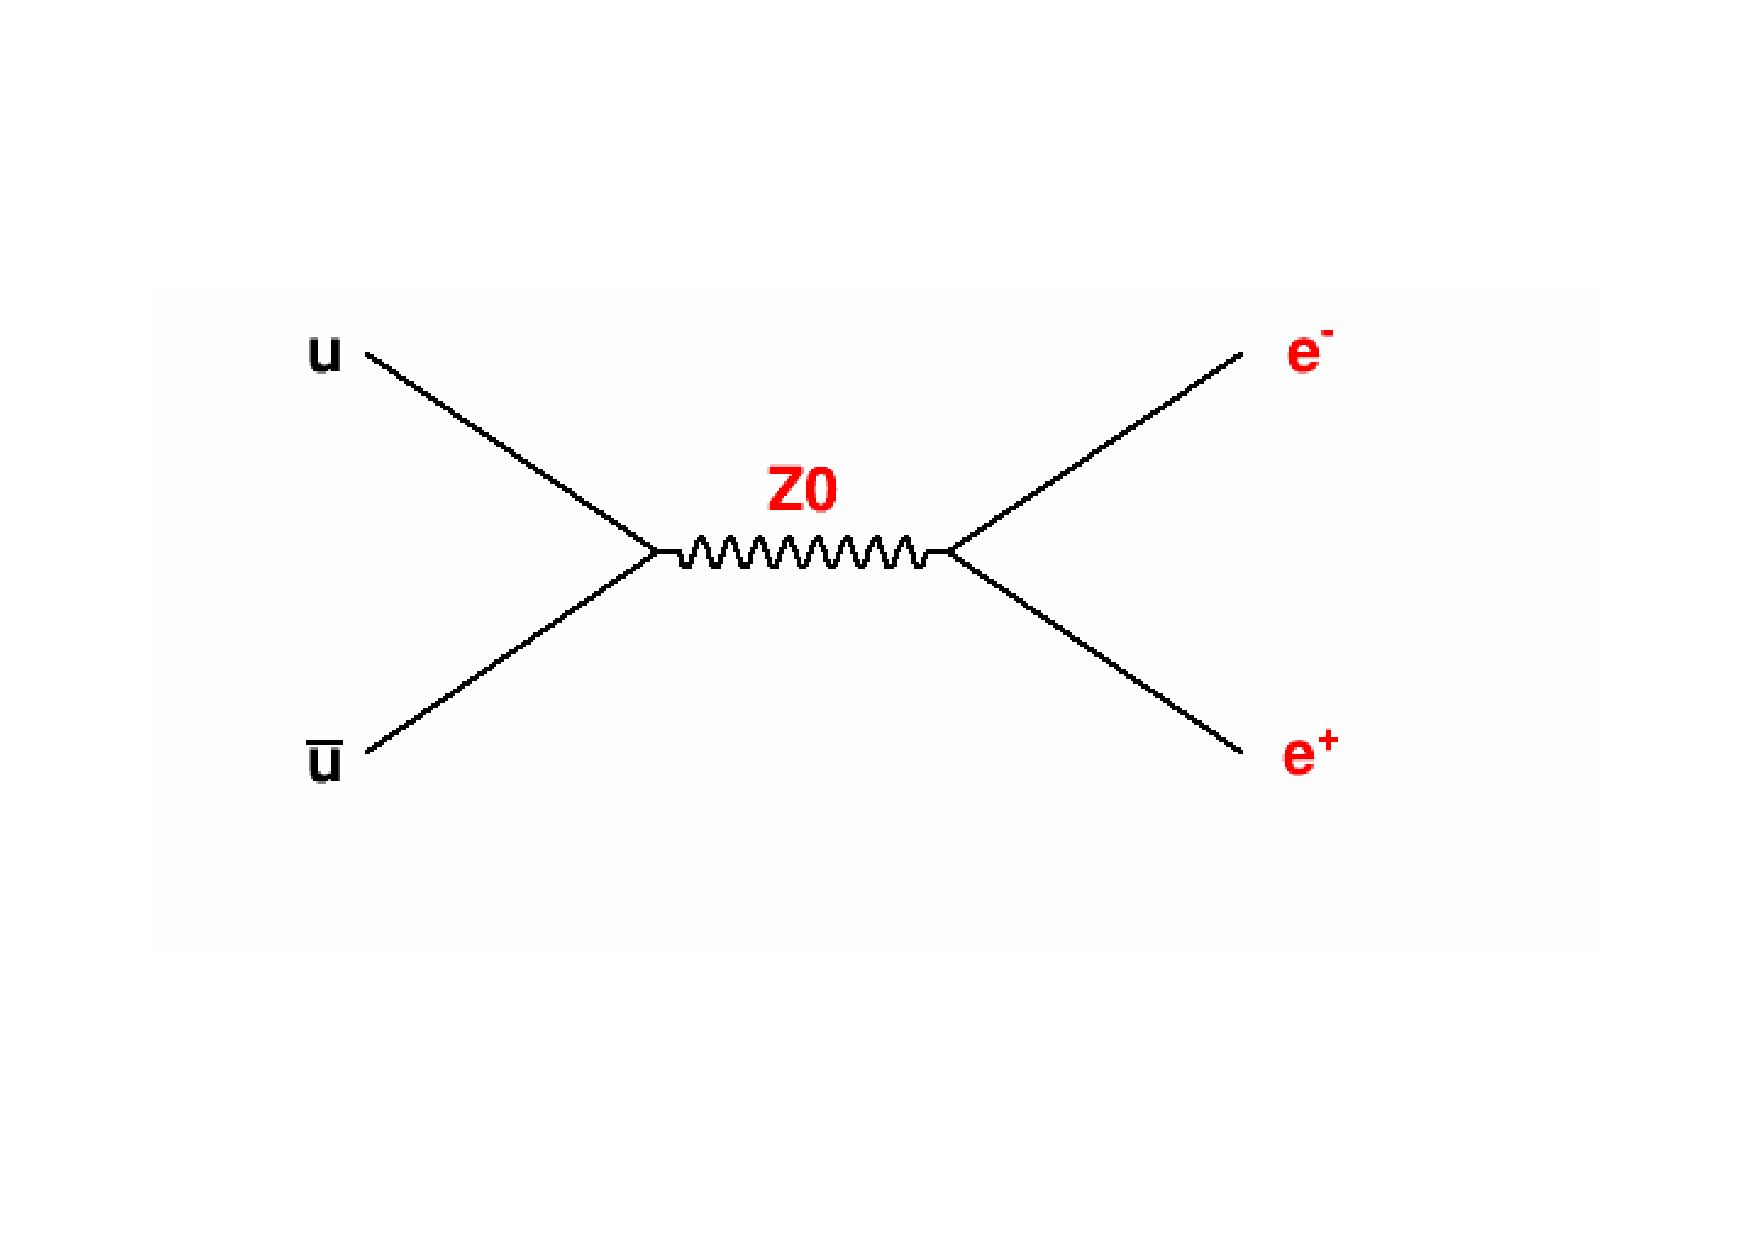
\includegraphics[scale=0.4]{./relativity/Pictures/FeynmannDiagram.pdf}
\caption{Feynman diagram for production of a Z boson in a proton-proton collision, with subsequent decay to electrons}
\label{fig:collrel}
\end{figure}




The total momentum of the proton is divided among the partons in an unequal way that varies collision by collision.  Sometimes most of the momentum is held by a single parton.  Sometimes it is divided among a very large number of partons.  We can know the distribution of probabilities versus fraction of proton momenta, but cannot know, for a specific collision, what fractions the colliding partons had.  It will be very rare, however, for both partons to have equal but opposite momenta in the lab frame.

It is usually easiest to understand this collision if we transform to the frame where the partons do have equal but opposite momenta.  This special frame is called the center-of-mass frame.  In this frame, the partons have equal but opposite 3-momenta.  The total initial state 2-momenta, therefore, is zero.  Since momentum is conserved, this means the Z boson produced must have zero 3-momenta and therefore zero kinetic energy.  Its only energy will be that due to its mass.  Since energy is also conserved, this means the initial energies of the partons must be half the Z mass (ignoring for now the finite width of the Z).  Since the partons are approximately massless, this means that the initial momenta of the partons must be:

\begin{equation}
 p_{u} = ( {M_z \over 2},0,0,{M_z \over 2})
\end{equation}
\begin{equation}
 p_{\bar{u}} = ( {M_z \over 2},0,0,-{M_z \over 2})
\end{equation}

\noindent What about the electrons that are produced?  Again, due to conservation of momentum, their 3-momenta must be equal and opposite.  And, from conservation of energy, their energies must be half the Z mass.  Because they are approximately massless, the magnitude of their 3-momenta must be equal to their energy.  However, their 3 momenta do not have to be along the z axis.  So, in general:

\begin{equation}
 p_{e^+} = (\frac{M_Z}{2}, \frac{M_Z}{2} cos \theta cos \phi ,  \frac{M_Z}{2} cos \theta sin \phi , \frac{M_Z}{2} sin \theta) 
\end{equation}
\begin{equation}
 p_{e^-} = (\frac{M_Z}{2}, \frac{M_Z}{2} cos (\pi - \theta) cos \phi ,  \frac{M_Z}{2} cos  (\pi - \theta) sin \phi , \frac{M_Z}{2} sin  (\pi - \theta)) 
\end{equation}


	  
The probability distribution for the polar and azimuthal angles are predicted by the standard model, but is beyond the level of this course.

What will this look like in the lab frame?

Since to boost back into the lab frame, we do a boost along the z axis, only the z components of 3-momentum will change.  The x and y components will stay the same.  The energy will change as well, since (in the massless, highly relativistic approximation)
\begin{equation}
E^2 = p_x^2 + p_y^2 + p_z^2   
\end{equation}
The polar angle changes, but the azimuthal angle does not.  Because of this, transverse variables are very important to collider physicists; they are most sensitive to the particle produced, and not sensitive to the boost.

The component of momentum transverse to the beam axis is called the {\it transverse momentum}.  It's magnitude is calculated:
\begin{equation}
	 p_T =   \sqrt{p_x^2 +p_y^2}
\end{equation} 
  

You will see this variable over and over when you work on hadron collider physics.

\section{Rapidity and Pseudorapidity}
As we will discuss in more detail later, the kinematics of particle production and decay have an interesting property.  If a particle is produced at rest, and it decays to two daughter particles (what conservations laws prevent it from decaying to one daughter particle?), conservation of momentum requires the two daughters to be back-to-back and have the same momentum.  At the LHC, however, as we will see, new particle are not produced at rest.  They will usually be produced with a velocity along the beam (z) direction.  We of course can do any calculations in the frame where the produced particle is at rest (a frame moving with the same velocity of the produced particle), where they are easy to do, but then to predict what we will see in the lab, we will need to transform back to the lab frame.

It is nice to use variables that have simple transformation properties.  Therefore, two variables are very common in experiments involving proton collision: rapidity and pseudorapidity.  They have much nicer transformation properties (as you will explore in your Homework) than the normal polar angle ${\rm \theta}$.


Rapidity is defined as:

\begin{equation}
	 y =  \frac{1}{2} ln (\frac{E + p_z}{E-p_z})
\end{equation} 
	  

\vspace{.2cm} 
\begin{minipage}{0.9\textwidth} 
\begin{framed}
%\vspace{.1cm}
\begin{exercise}
%\begin{frshaded}
%\fcolorbox{\bordercolor}{\backgroundcolor} 
{show that the difference in rapidity between two particles is independent of the boost in the z direction.}
\end{exercise}
%\end{frshaded}
%\vspace{.1cm}
\end{framed} 
\end{minipage}
\vspace{.2cm}




A related variable is the pseudorapidity, defined as:

\begin{equation}
	 \eta  = - \ln{\tan{\frac{\theta}{2}}}
\end{equation} 


\vspace{.2cm} 
\begin{minipage}{0.9\textwidth} 
\begin{framed}
%\vspace{.1cm}
\begin{exercise}
%\begin{frshaded}
%\fcolorbox{\bordercolor}{\backgroundcolor} 
{show that rapidity and pseudorapidity are equal for massless particles.}
\end{exercise}
%\end{frshaded}
%\vspace{.1cm}
\end{framed} 
\end{minipage}
\vspace{.2cm}



\section{Further reading}
\begin{itemize}	
\item http://en.wikibooks.org/wiki/Special\_Relativity
\end{itemize}



%----------------------------------------------------------------------------------------
%	CHAPTER 3
%----------------------------------------------------------------------------------------
\chapterimage{Pictures/chapter_head_2.pdf} % Chapter heading image
\chapter{Particle Interactions with matter}

\section{Introduction}\index{Introduction}

The purpose of a particle physics detector is to find all the particles produced
in a collision, identify their types, and measure their 4-momenta.
At the LHC, in a single collision, thousands of particles can be produced.
The particle physics detector must make signals that somehow can yield this information.
To understand how this can happen, we first must understand how particles interact
with matter, so we can learn of the possible types of signals particles can produce.

What kinds of particles can the LHC detector detect?  First, the particle must live long 
enough to reach the detector without decaying.  The beam pipe of the LHC has a 
radius with dimensions measured in cm.  The particle must exist long enough to escape the beam pipe and
reach the detector and make a signal.  If we take the diameter to be 1 cm, then
the particle life time must be large enough to travel this far before decay.
How far does a particle travel before decaying?  We learned in Chapter \ref{EP} that fraction remaining after a time $t_0$ is given by
\begin{equation}
N=N_0 e^{-t_0 \over \tau}
\end{equation}
The probability of surviving is $N / N_0$ so
\begin{equation}
P(t)= e^{-t_0 \over \tau}
\end{equation}
To change this to the probability of traveling a distance instead of a time, remember that, with relativity, the lifetime for a moving particle depends on the lifetime for the particle at rest as $\tau = \gamma \tau_0$ so we have
 \begin{equation}
P(t)=e^{-t_0 \over {\gamma \tau_0}}
\end{equation}
Position is then related to time by $x_0=vt_0$ or $x_0=\beta c t_0$, so
\begin{equation}
P(t)=e^{-x_0 \over {\beta c \gamma \tau_0}}
\end{equation}
Then, using
$\Gamma=\hbar/\tau_0$, $\gamma=E/mc^2$ where m is the particle's mass 
and $\beta=pc/E$, we have
\begin{equation}
P(x_0)=e^{{-x_0\Gamma mc^2}\over{pc\hbar c}}
\end{equation}

The particle must also interact  with matter in a way that produces a large enough signal to measure in a detector that is small enough to be affordable.  While specialized very large detectors exist which can detect neutrinos, this is not possible at a collider detector.

There are only a few types of particles (and their antiparticles) that satisfy these requirements, and they are: from the leptons: electrons and muons; from the bosons: photons; from the mesons:
charged pions, charged kaons (remember: these contain a strange quark), k-longs (a type of rare kaon; kaons, as you remember are mesons containing a strange quark); From the baryons: protons, neutrons.

The most common particle produced in a proton-proton collision is the pion.  Neutral pions decay very quickly to two photons. Most of the particles we detect, therefore, will be charged pions and photons.  However, as we will discuss, particles like electrons and muons are signatures of Higgs decays, and so we need to have a detector well optimized for identifying and measuring these particles as well.




\section{Interactions of charged particles with matter}\index{chargedinteractions}
We will first look at possible signals from charged particles (electrons, muons, charged pions, protons).

Possible interactions between these particles and bulk matter include:
\begin{itemize}
\item ionization and excitation of the molecules in the material
\item multiple scattering
\item bremsstrahlung
\item strong interactions with atomic nucleii (only for mesons and baryons, as these contain quarks)
\end{itemize}
We will postpone the discussion of the last two of these interactions until our discussion of ``calorimetry''.

When a charged particle passes through some material (detectors are often made of Argon gas, silicon, iron, lead, steel, plastic, and other such materials), it will interact with the electrons in the molecules that make up that material via the electric force.  
The charged particle loses energy as it passes through the material, and the material gains energy.  
It is somewhat similar to sliding friction. For example, when a book slides across a table, the molecules in the book interact with those on the table via the electric force.  This causes the kinetic energy of the book to decrease, and become heat energy in the book and the table.  This heat energy, you may remember, is associated with the random, invisible motion of the molecules in the book and table.  There is a difference though.  The energy of the charged particle doesn't initially produce heat (although, eventually, some heating can occur.)
What effect does that energy have on the material?  It can cause the electrons in the material to ``be excited'' into higher quantum states or it can even detach an electron from its atom (``ionization'').  This excitation energy can eventually turn into heat energy or it can produce signals that can be detected, as we will discuss later.

We are often interested in how much energy the particle loses (material gains) per unit length.  This is called $dE/dx$, pronounced ``d-E-d-x''.    The average amount of energy lost per unit length depends on the energy of the particle: low energy particles lose more energy per unit length than high energy particles.  You can imagine why this might be true: the lower energy (slower) particles linger near each atom in the material longer, and thus have a longer time to interact with each one and lose more energy.  The energy loss per unit length decreases as $1/\beta^2$ until a momentum around 0.1 GeV, where it has its minimum value.  The loss then increases slowly with increasing energy until about 100 GeV.  Above this energy, relativistic effects cause dEdx to increase more quickly with energy.  Particles in the momentum range of 0.1 to 100 GeV are called "minimum ionizing particles" or "mips".

Figure ~\ref{fig:pdgdedx} shows the energy dependence of dEdx for various charged particles.  Note that the 
units are
strange. You might expect, since dEdx is energy per length, the units to be ${\rm MeV/cm}$.  Instead, they are ${\rm Mev {cm^2 \over g} }$.
You can convert this to a more convention unit by multiplying by the density of the material
\begin{equation}
{{MeV cm^2}\over{g}} \cdot {{g}\over{cm^3}} = {{MeV}\over{cm}}
\end{equation}
The reason the authors use these units is that it allows the dEdx curves for high Z and low Z elements to fit onto the same graph.

\begin{figure}[h]
\centering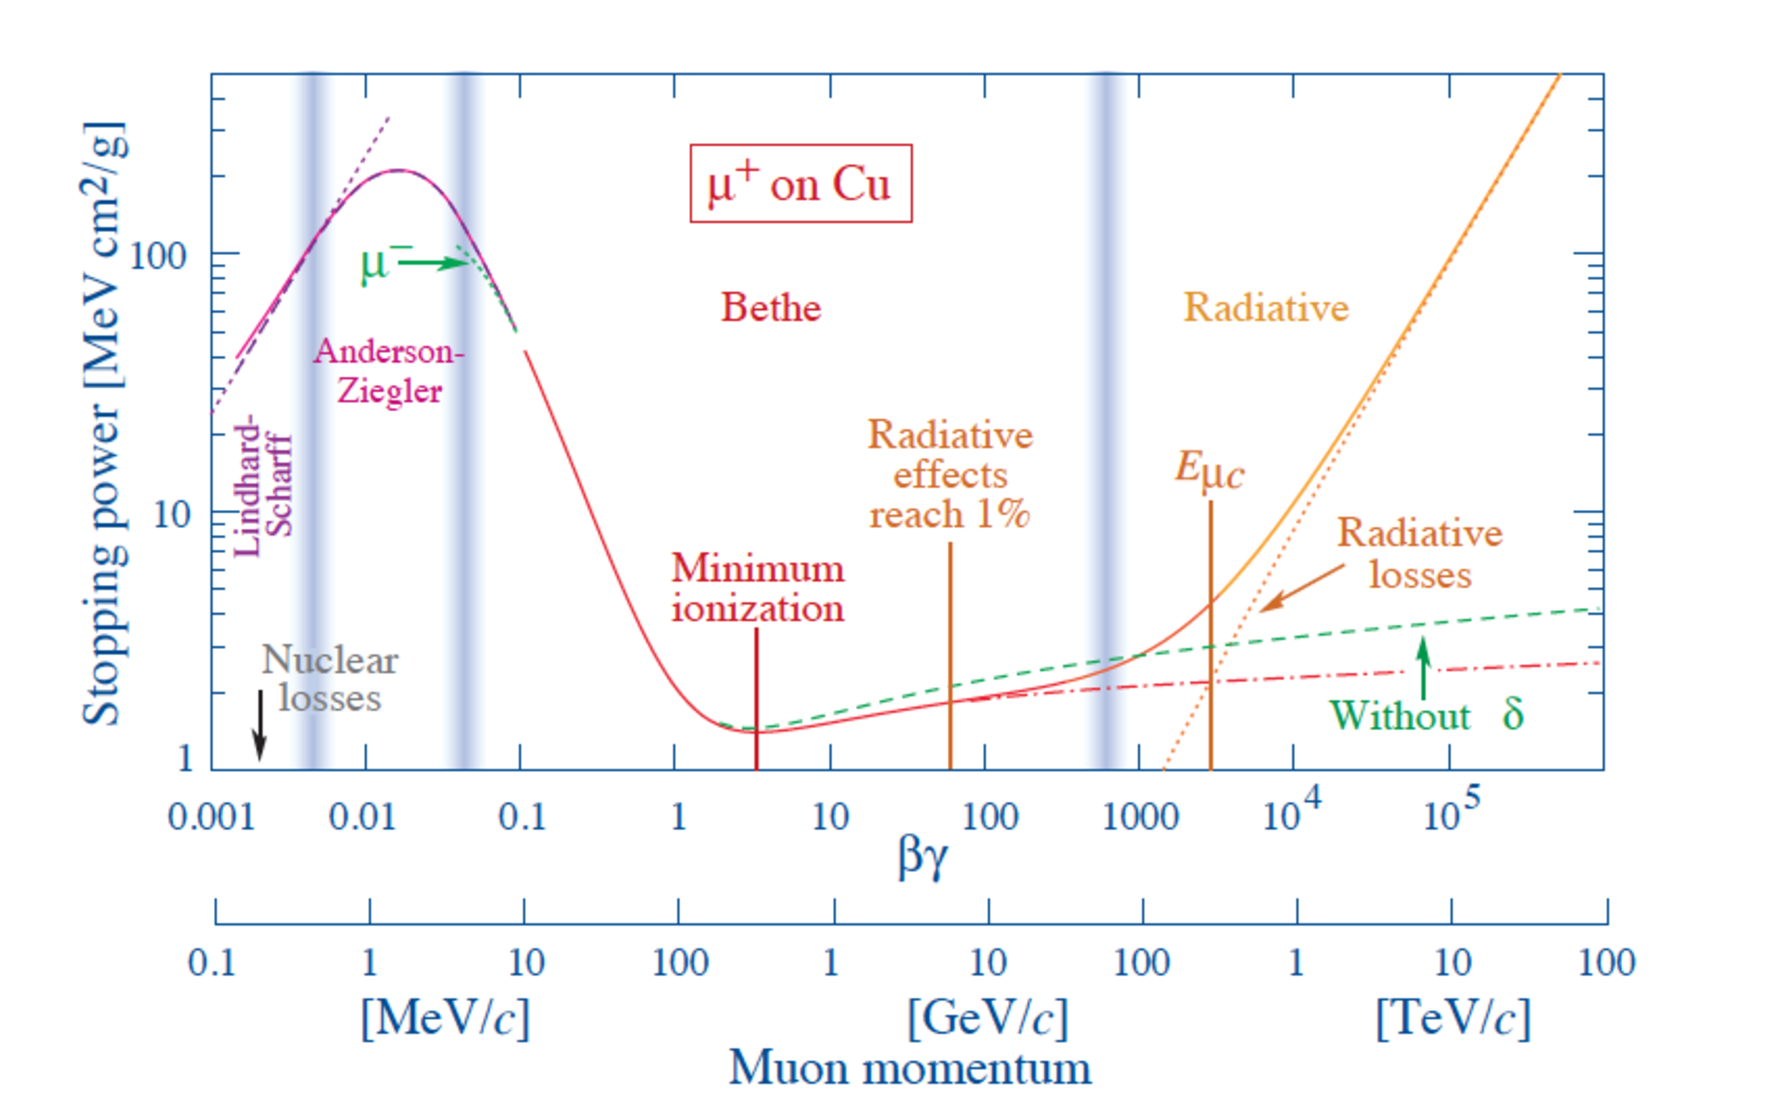
\includegraphics[scale=0.5]{./particleinteractions/Pictures/dedx.pdf}
\caption{Stolen from the particle data group, this picture shows the energy
loss per unit length as a function of particle energy}
\label{fig:pdgdedx}
\end{figure}

What kind of signals can be produced this way?  If the material is a gas, the electrons produced through ionization can be gathered on a wire (using an electric field produced by voltages on metal pads on the structure holding the gas or on wires running through the gas) to produce a current.  The signals from silicon are similar.  If the material is a plastic scintilator, some of the ``excited'' molecules will ``de-excite'' by emitting photons, which can be detected with a photomulitplier tube or other light sensitive device.

If the material is thick and high-Z (iron, lead), the particle may lose all its energy and 
stop inside the material.  The thickness of material that will stop a particle (of a given energy) is called the particle's range.  Fig~\ref{fig:pdgrange} shows the range for various particles in various materials as a function of particle energy.


\begin{figure}[h]
\centering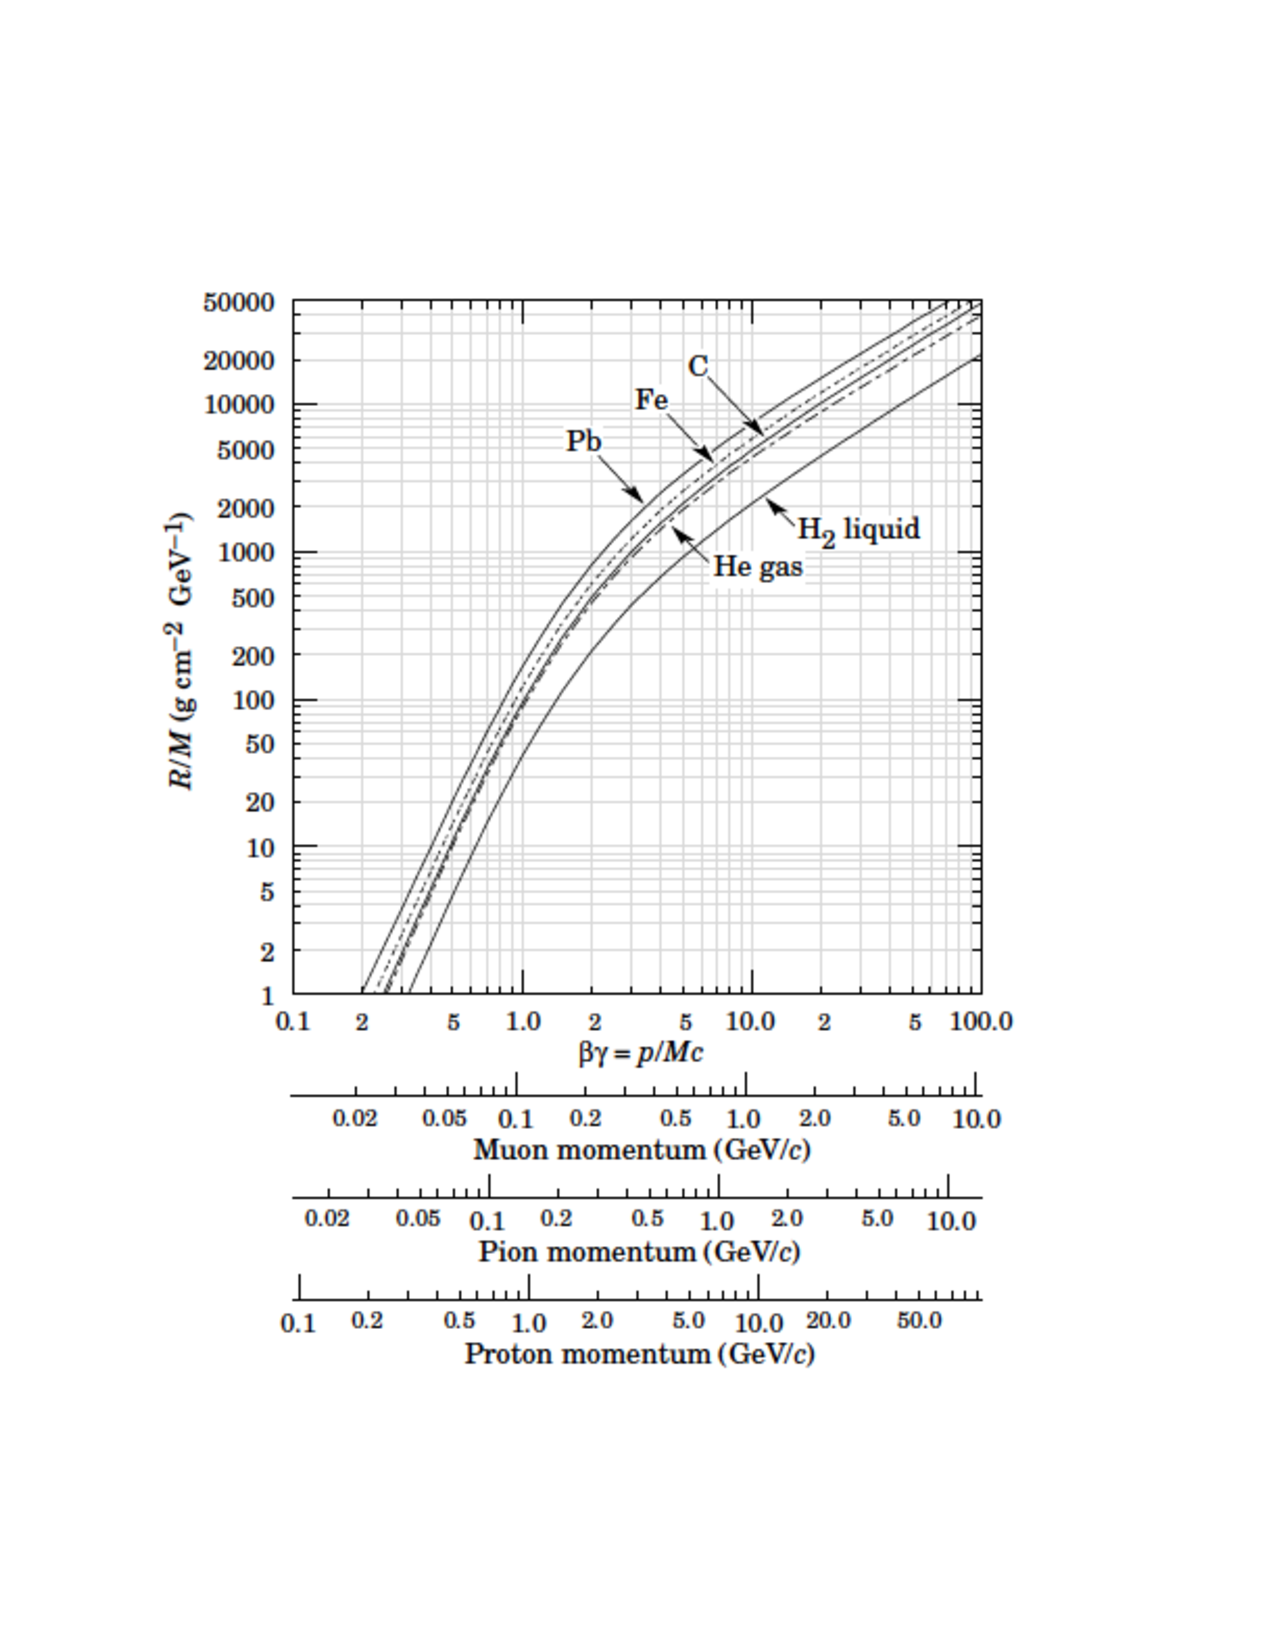
\includegraphics[scale=0.5]{./particleinteractions/Pictures/pdgrange.pdf}
\caption{Stolen from the particle data group, this picture shows the range of a particle in various materials as a function of particle energy }
\label{fig:pdgrange}
\end{figure}

Of course, because each particle that goes through the material will randomly interact with different numbers of atomic electrons, exchanging more energy when it happens to go close to one, and exchanging less when it is further away, particle by particle the amount of energy varies.  The distribution of deposited energies follows a "Landau" distribution, as shown in Fig~\ref{fig:landau}.


\begin{figure}[h]
\centering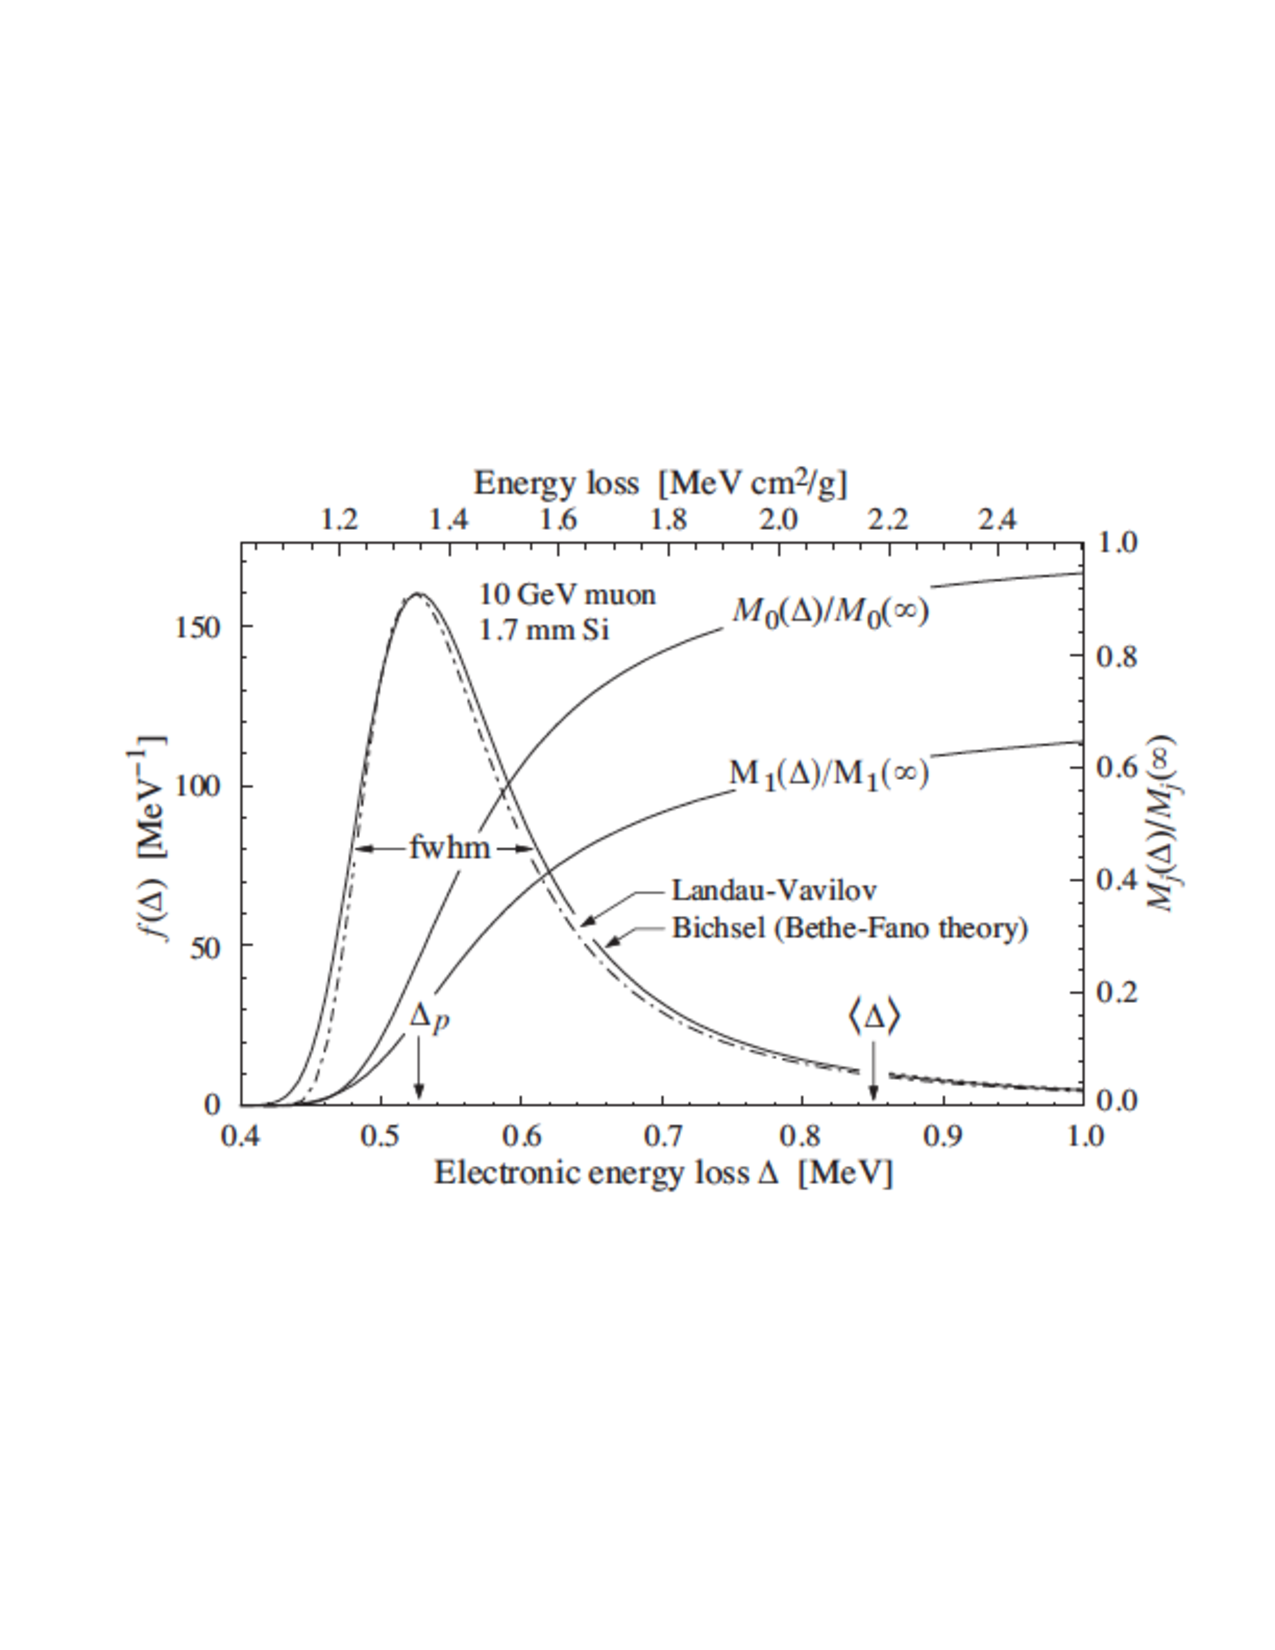
\includegraphics[scale=0.5]{./particleinteractions/Pictures/landau.pdf}
\caption{Stolen from the particle data group, this picture shows the distribution of energy deposits for a 10 GeV muon transversing 1.7 mm of silicon. }
\label{fig:landau}
\end{figure}

Sometimes a particle passes close enough to an atom to interact with the nucleus, instead of the electrons.  The mass of the nucleus, and the force binding it into its places in the crystal lattice, are large compared to the mass of the particle.  The particle usually bounces off the nucleus the way a ball bounces off a wall, changing direction, but without losing energy.  For a material that is not very thin, this can happen multiple times, and thus this is called "multiple scattering".  Fig~\ref{fig:pdgmultscattcartoon} shows a cartoon of this process.


\begin{figure}[h]
\centering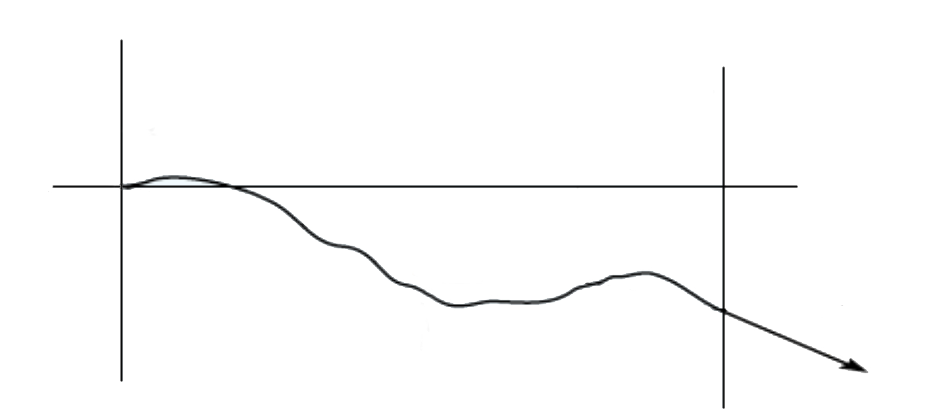
\includegraphics[scale=0.5]{./particleinteractions/Pictures/multscattcartoon.pdf}
\caption{Stolen from the particle data group, this picture shows a cartoon showing the path of a charged particle undergoing multiple scattering in matter }
\label{fig:pdgmultscattcartoon}
\end{figure}



\section{Interactions of gamma rays with matter}\index{gammainteractions}

Here, we call them “gamma rays” instead of photons because we are going to discuss only those photons of interest to particle physics: ones with energies above a keV or so.

There are several ways a gamma ray can interaction with matter:
\begin{itemize}
\item photoelectric effect
\item Compton scattering
\item pair production in the field of the nucleus
\item pair production in the field of the electron
\item photonuclear interactions
\end{itemize}

The photoelectric effect was very important in the development of quantum mechanics.  Einstein was awarded the Nobel Prize for his work on its understanding.  It is an interaction between a photon and an atom electron.  If the photon has energy greater than the binding energy of the electron to the atom, it can eject the electron.  The electron will have a kinetic energy equal to the energy of the photon minus the binding energy.


Compton scattering is the scattering of a photon off an electron.  The Feynman diagram is shown in Figure ~\ref{fig:compton}. 


\begin{figure}[h]
\centering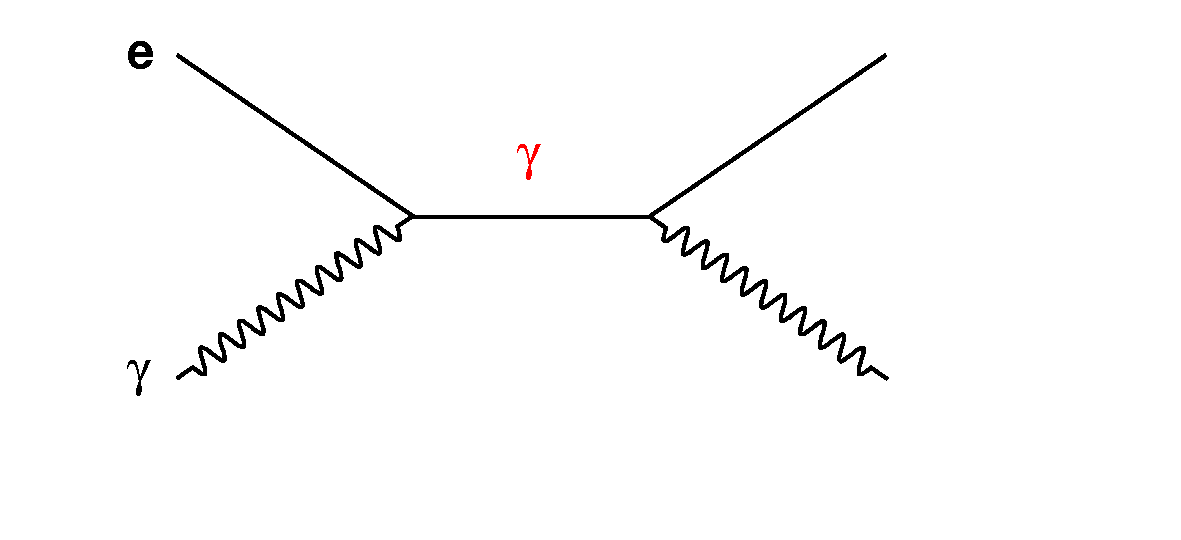
\includegraphics[scale=0.5]{./particleinteractions/Pictures/compton.pdf}
\caption{Feynmann diagram for Compton scattering of a photon by an electron}
\label{fig:compton}
\end{figure}

Pair production is the conversion of a photon into an electron-position pair through an interaction (usually) with a nucleus.  The Feynmann diagram is shown below.


\begin{figure}[h]
\centering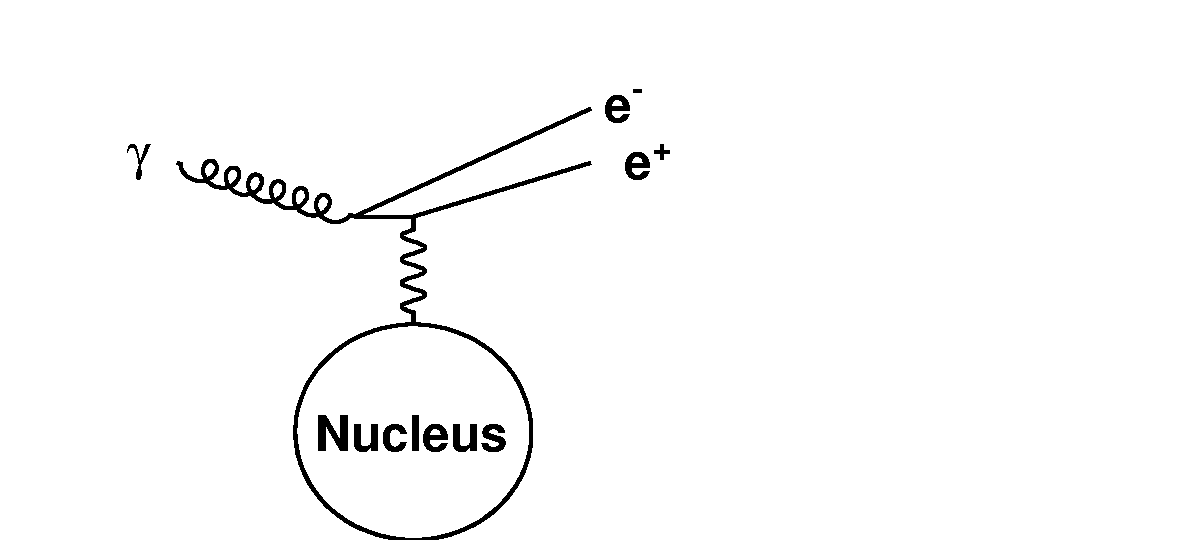
\includegraphics[scale=0.5]{./particleinteractions/Pictures/pairproduction.pdf}
\caption{Feynmann diagram for pair production in the field of a nucleus}
\label{fig:pairproduction}
\end{figure}



Figure~\ref{fig:photoninteractions} shows the cross section for each mechanism as a 
function of photon energy.  As you can see, for photons with energy greater than twice the 
electron mass, pair production is the most important mechanism.  We will discuss this in more detail when we discuss calorimetry.


\begin{figure}[h]
\centering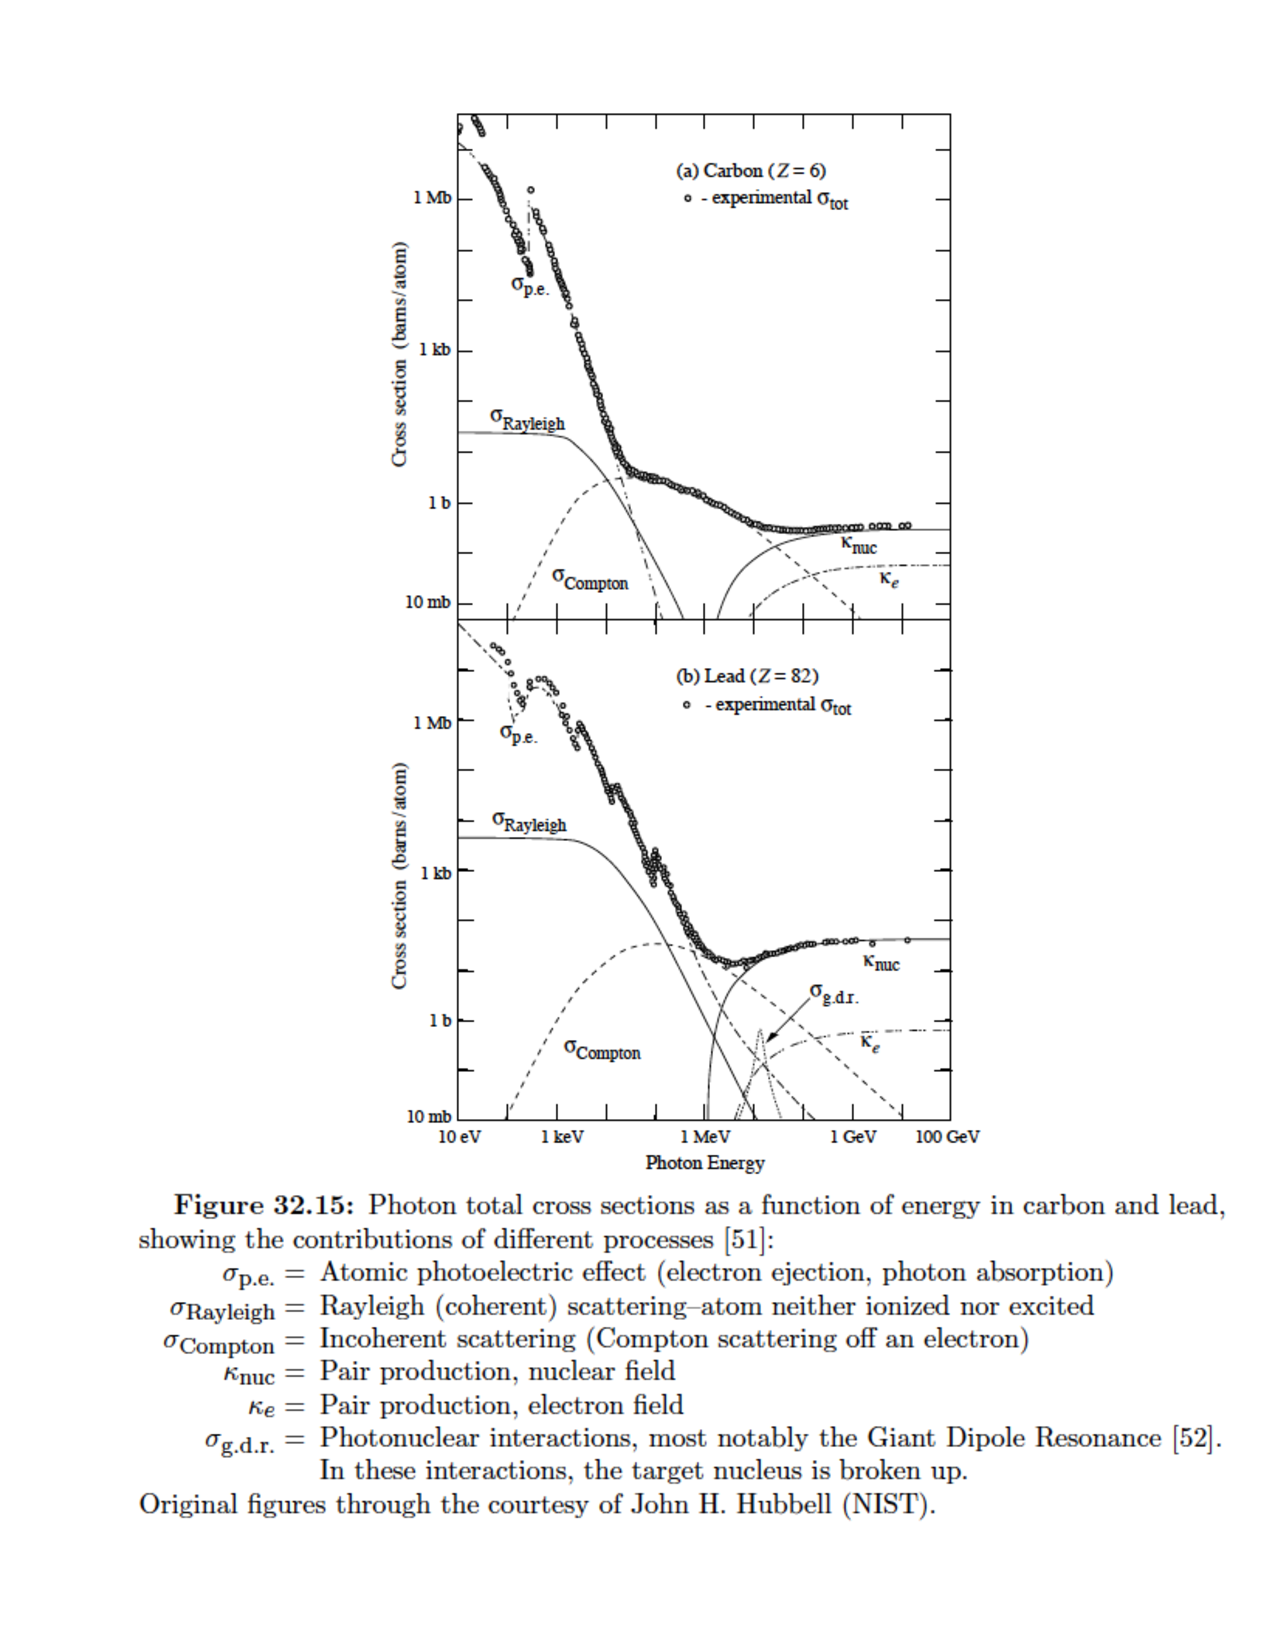
\includegraphics[scale=0.5]{./particleinteractions/Pictures/photoninteractions.pdf}
\caption{Stolen from the particle data group, this picture shows the cross sections for possible interactions of photons with matter as a function of photon energy }
\label{fig:photoninteractions}
\end{figure}



%----------------------------------------------------------------------------------------
%	CHAPTER 4
%----------------------------------------------------------------------------------------
\chapterimage{Pictures/chapter_head_2.pdf} % Chapter heading image
\chapter{Statistics}

\section{Statistics}\index{Statistics}

Please read chapter 3.I to 3.V in
\url https://archive.org/download/pdfy-KjqMaZQFCJ7PUQgp/Knoll-Glenn-F-Knoll-Radiation-Detection-Measurement-3rd.pdf







%----------------------------------------------------------------------------------------
%	CHAPTER 5
%----------------------------------------------------------------------------------------
\chapterimage{Pictures/chapter_head_2.pdf} % Chapter heading image
\chapter{Particle accelerators}
test test

%----------------------------------------------------------------------------------------
%	CHAPTER 6
%----------------------------------------------------------------------------------------
\chapterimage{Pictures/chapter_head_2.pdf} % Chapter heading image
\chapter{Calorimeters}
\section{Basic Idea}

\noindent
The goal of a particle physics detector is to measure the 4-momenta of all particles produced in a collision and to identify their types.  As we discussed in the section on tracking, the 4-momenta of charged particles, such as electrons, pions, etc... whose $\left | \eta  \right |$ is not too large (usually less than about 2) can be measured by the tracker. However, we need another way to measure electrically neutral particles or ones at large. However, we need another way to measure electrically neutral particles or ones at large $\left | \eta  \right |$.

\;
\noindent
You may have already encountered the word ``calorimeter'' in your high school physics.  In thermodynamics, the temperature of a known (hot) object may be measured by immersing it in a bath and measuring the temperature rise of the bath.  The heat energy of the unknown object becomes that of a known object, allowing measurement. In a HEP calorimeter, the goal is to turn the kinetic energy of the particle into another type of energy that is more easily measured. In the process, the particle is altered so that it no longer reflects its initial properties (especially the momentum, but sometimes the type is changed) and no further useful measurements can be made.  Calorimeters should therefore be outside of the non-destructive detectors.

\;
\noindent
Remember our goal is to identify the 4-momentum and identify the type of all particles produced in the collisions. In a calorimeter, as we will discuss later, we can often use the shape of the energy deposit to tell if the particle is  either an electron or a photon (on the one hand) or a hadron. The calorimeter is segmented so the azimuthal ($\phi$) and polar angle ($\theta$) can be estimated, assuming the particle was produced at the center of the detector, by drawing a line from the production point to the impact point on the calorimeter face. If we assume the particle$'$s mass is small compared to its momentum (massless approximation), the particle$'$s momentum can be estimated as:

\begin{equation}\hspace{34 mm}p = E(l,cos(\theta ),cos(\phi ),cos(\theta ),sin(\phi ),sin(\theta ))\end{equation}

\;
\;

\section{Showers}

\noindent
In a particle physics calorimeter, we try to first change the neutral particles (photons, neutrons, K-longs) into charged particles. Then, we change single high energy charged particle into a very large number of low energy charged particles in such a way that the number we create is proportional to the kinetic energy of the initial high energy particle. The low energy charged particles travel through matter, interacting with the electrons in the material, transferring their kinetic energy to them, until all the initial kinetic energy is transferred to the material. That material then needs to make some kind of signal that can be detected. You can see a schematic of this process in figure ~\ref{fig:cal1}. An initial particle comes in, somehow interacting with the material of the calorimeter, and is changed gradually into a large number of low energy particles, that ``range out'' in the material. This process is called ``showering''.

\;
\;

\begin{figure}[h]
\centering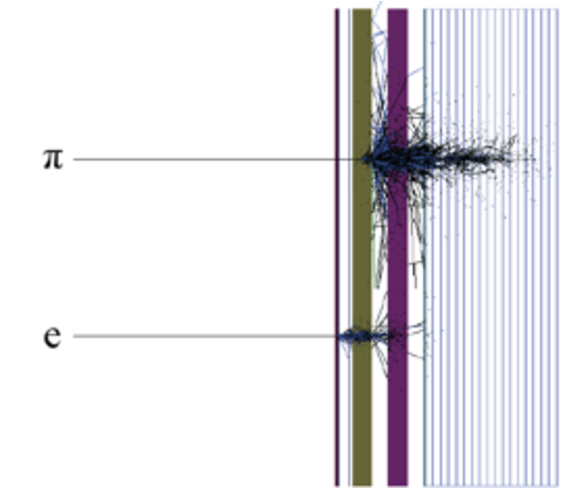
\includegraphics[scale=1.0]{./calorimetry/Pictures/fig1.pdf}
\caption{Schematic of a typical calorimeter. The front part is the ``Electromagnetic'' calorimeter and should contain the showers resulting from electrons and photons. The back of the calorimeter is the ``hadronic'' part, and should contain the showers resulting from particles containing quarks (mesons, baryons, etc).}
\label{fig:cal1}
\end{figure}

\;

\noindent
What are the processes that cause the creation of the secondary particles? That depends on whether the initial high energy particle was an ``EM'' particle (an electron or a photon) or a ``HAD'' particle (mesons, baryons).

\section{Electromagnetic Showers}

\noindent
An electromagnetic shower results when an electron or photon enters a thick piece of material with a large atomic number (Z). There are two main processes that occur: Bremssrahlung and pair production.


\noindent
Bremsstrahlung is German for ``braking radiation'', and is a process that occurs for electrons. As you may have learned in your high school physics course, when a charged particle accelerates, it radiates electromagnetic radiation (photons, the particle of light). What would cause an electron to accelerate? An electron is a charged particle. A nucleus is also charged. For nuclei, such as lead or iron, that charge can be large. If an electron passes close enough to a nucleus, the electric force between the two particles causes the electron to accelerate (because the nucleus is much heavier than the electron, and is bound in the lattice of the solid, it does not move). Thus, in the presence of the nucleus, a high energy electron becomes a lower energy electron and a gamma ray (high energy photons). This can be draw as shown in figure ~\ref{fig:cal2}


\;
\;

\begin{figure}[h]
\centering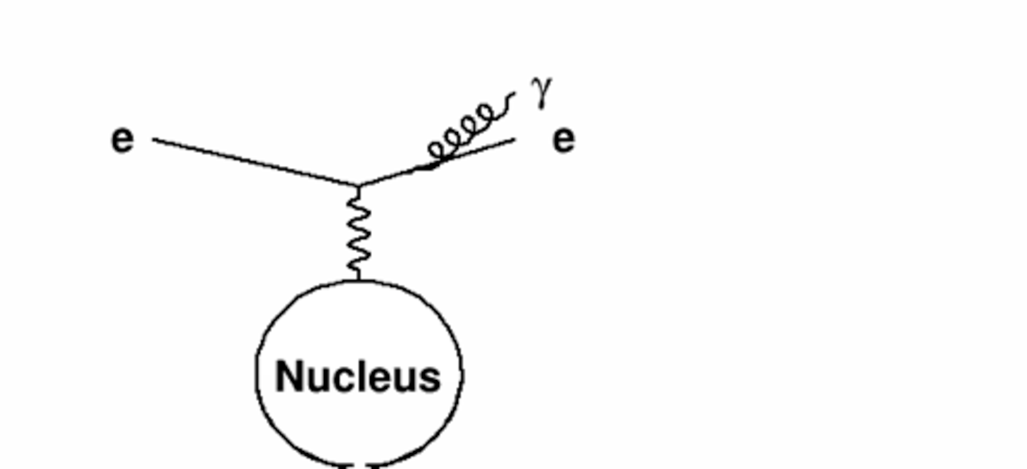
\includegraphics[scale=0.7]{./calorimetry/Pictures/fig2.pdf}
\caption{An electron radiates off a gamma ray in the presence of a nucleus.}
\label{fig:cal2}
\end{figure}

\;


\noindent
A similar process allows a high energy photon to become an electron-positron pair.  The energy of the photon must be at least twice the electron mass in order for this to not violate conservation of energy.  The Feynman diagram is shown in figure \ref{fig:cal3}.


\;
\;

\begin{figure}[h]
\centering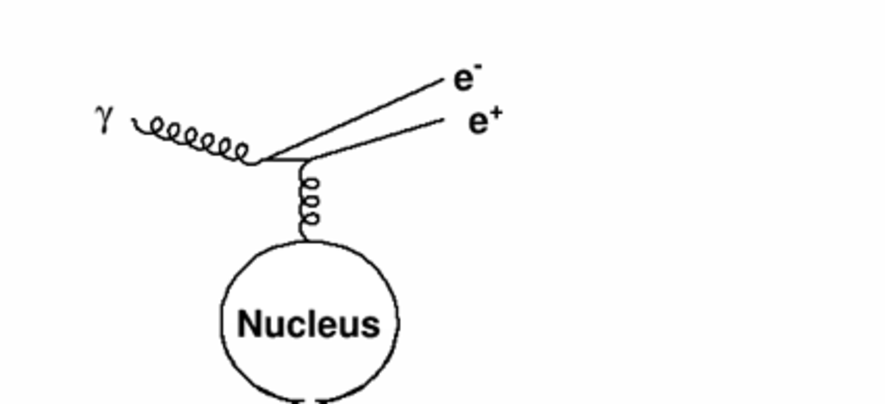
\includegraphics[scale=0.7]{./calorimetry/Pictures/fig3.pdf}
\caption{A high energy photon in the presence of a nucleus turns into an electron-positron pair}
\label{fig:cal3}
\end{figure}

\;

\section{Hadronic Showers}

\noindent
Electrons interact with the nucleus by producing electromagnetic interaction because of the electromagnetic force. Hadrons, however, can interact with nuclei via the strong force. This can cause a wide variety of processes to occur, often involving the break up of the nucleus. It takes more material to initiate a hadronic shower, as the hadron must pass closer to the nucleus, as the strong force is short range. A diagram of the resulting shower is shown in figure ~\ref{fig:cal4}

\;
\;

\begin{figure}[h]
\centering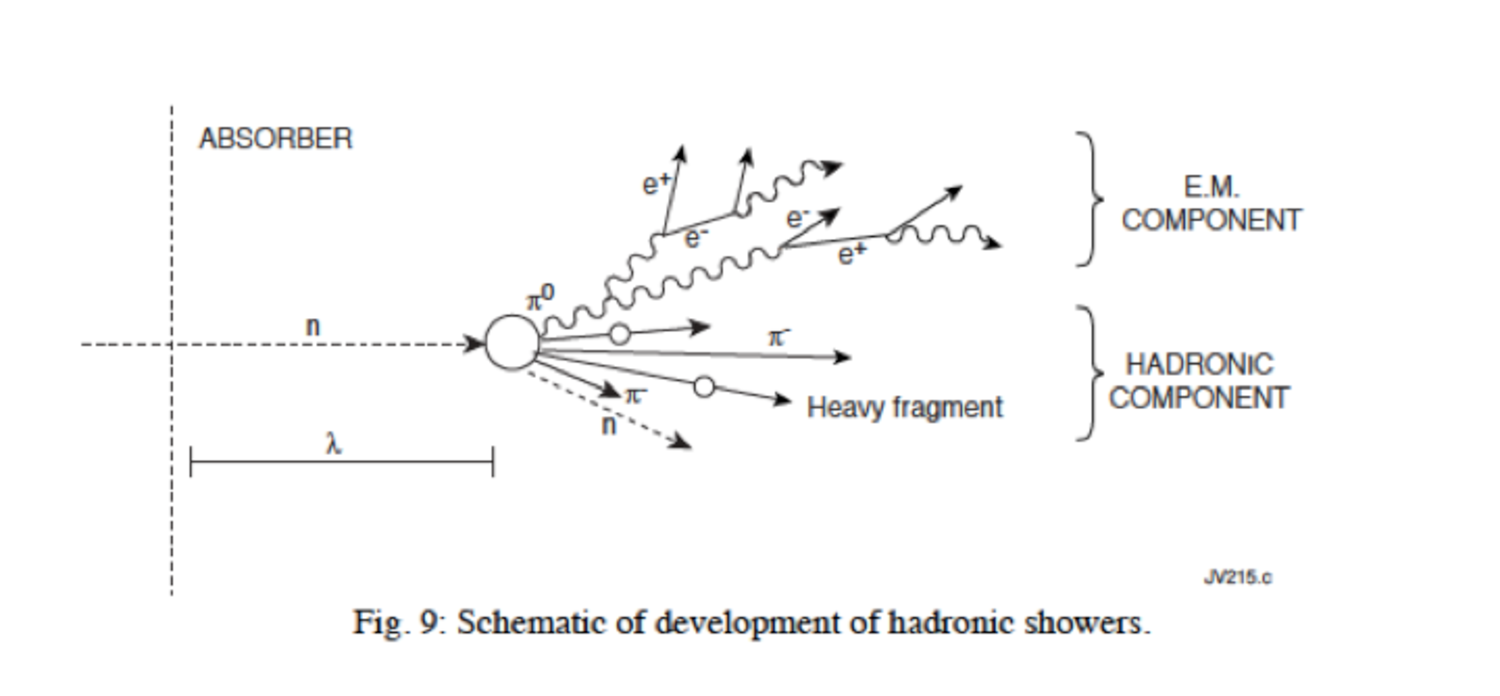
\includegraphics[scale=0.5]{./calorimetry/Pictures/fig4.pdf}
\caption{A figure showing a hadronic shower}
\label{fig:cal4}
\end{figure}

\;

\section{Detection}

\noindent
How do we measure the energy gained by the material? For many calorimeters, it is through the process of scintillation. Now, most high Z materials (think lead or uranium) do not scintillator, and are anyway opaque to light. So a calorimeter is often made of layers of the ``passive'' (high Z) material and the ``active'' (light producing) material, often plastic scintillator. A calorimeter that is like a smith island cake and has many layers is called a ``sampling'' calorimeter. The light produced by the scintillator is measuring using a photomultiplier tube or other light sensitive device (figure ~\ref{fig:cal5}).


\;
\;

\begin{figure}[h]
\centering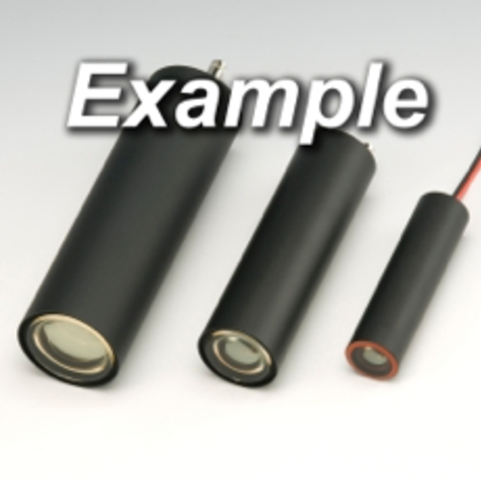
\includegraphics[scale=0.5]{./calorimetry/Pictures/fig5.pdf}
\caption{A picture of a PMT stolen from the web site of Hamamatsu corporation, one of the largest manufacturers of these devices.}
\label{fig:cal5}
\end{figure}

\;

\section{Sampling}

\noindent
Look at this picture of an EM shower in a sampling calorimeter.


\;
\;

\begin{figure}[h]
\centering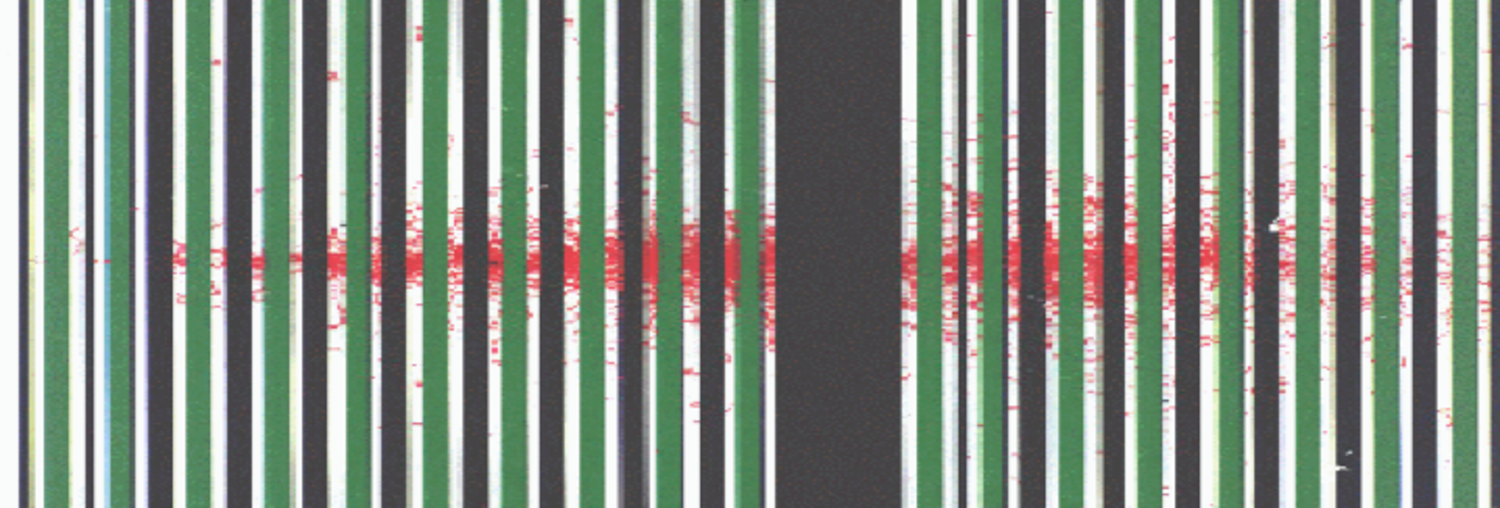
\includegraphics[scale=0.5]{./calorimetry/Pictures/fig6.pdf}
\caption{Schematic of an electromagnetic shower in a sampling calorimeter, as simulated by the GEANT4 shower simulation code. The colors denote various materials. The black denotes a high Z material, while the green denotes scintillator.}
\label{fig:cal6}
\end{figure}

\;

\noindent
The secondary particles only deposit some of their energy in the scintillator.  Most of it is deposited in the high Z material, which doesn$'$t produce light. Therefore, we are only measuring the energy of a small fraction of the shower, and thus a small fraction of the initial energy produced. We can correct for this on average:

\begin{equation}\hspace{34 mm}E_{estimated \: for \: initial\:  particle} = \frac{total \:amount\:  of\:  material \: in \: calorimeter}{amount \: of \: material\:  in \: plastic} E_{deposited \: in \: plastic}\end{equation}

\;
\;

\noindent
The ratio of the amounts of material is called the ``sampling fraction''. However, due to randomness in the shower process, sometimes a larger amount than this average will be deposited in the plastic, and sometimes less. This will lead to an uncertainty on the energy of the particle that started the shower. The smaller this ratio, the more accurate the measurement will be. For most calorimeters, though, the ratio is around 100.

\section{Energy Resolutions}

\noindent
How good is our calorimeter? This depends on how accurately it measures the energy of the initial particle. Sometimes, we take our calorimeters to test beams, and aim particles of known energy and momentum at them, to see how well they work. The figure below shows the result of aiming a beam of charged pions at the front face of the calorimeter.

\;
\;

\begin{figure}[h]
\centering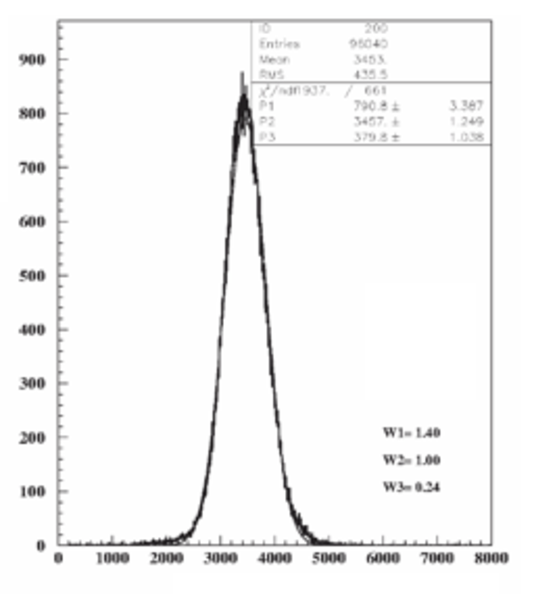
\includegraphics[scale=0.5]{./calorimetry/Pictures/fig7.pdf}
\caption{Charge collected from the detector when charged pions with a momentum of 300 GeV are steered into it.}
\label{fig:cal7}
\end{figure}

\;

\noindent
The output from the scintillator is charge, and so the x axis units are collected charge after amplification by the photomultiplier and other electronics. The detector is ``calibrated'' by setting the mean of this distribution (3457 fC) to the energy of the pions (300 GeV). The ratio of these numbers can be used to estimate the energy of the particle from the charge collected from the shower.  Of course, this is a very simplistic calibration. Getting an accurate calibration over a wide range of particle energies is a subject that could be a book in and of itself. 

\;
\noindent
As you can see, however, even though the incident particle always had the same energy, the amount of charge collected is not always the same. This is (mainly) because there are random fluctuations between the amount of energy deposited in the passive material and that deposited in the active material. The distribution of measured energies is well approximated by a Gaussian distribution:

\begin{equation}\hspace{20 mm}f(x,\mu,\sigma^{2}) = \frac{1}{\sigma\sqrt{2\pi }}\: e^{-(x-\mu)^{2}/2\sigma^{2}}\end{equation}

\;
\;

\noindent
The parameter $\mu$ is the mean of the distribution. The parameter $\sigma$ is the ``root mean square'' or ``sigma'' or the ``resolution''. It is a measure of the calorimeters ability to accurately measure the energy of the particle. In this figure, the mean is 3457 and sigma is 379.8. The fractional resolution is then the ratio of these two numbers, or 0.11.

\;
\noindent
The resolution for a calorimeter depends on the energy of the particle. The total number of secondary particles produced that cross the active material is proportional to the energy of the incident particle. The fluctuations on this number are proportional to the square root of this number, x. The fraction resolution (resolution/means) is thus proportional to $1/\sqrt{x}$.

\;
\noindent
There are other sources of resolution besides this, and so for a realistic calorimeter, the resolution is given by:

\begin{equation}\hspace{35 mm}\frac{\sigma }{E} = \frac{s}{\sqrt{E}} \oplus \frac{n}{E} \oplus C
\end{equation}

\;
\;

where s is called the ``sampling term'' and comes from the mechanism we discussed, n is called the ``noise term'' and is usually dominated by fluctuations in the measured charge due to electronics noise, and c is called the constant term, and is usually dominated by leakage of secondary particles out the back of the detector. The $\oplus$ symbol means ``add in quadrature''. To do this, square each term, add these squares, and take the square root.  As you learn more statistics, you will learn this is a common procedure when there is more than one source of randomness contributing to a measureable outcome.

\noindent The figure below shows the resolution versus energy for one of the CMS detector$'$s calorimeters.

\;
\;

\begin{figure}[h]
\centering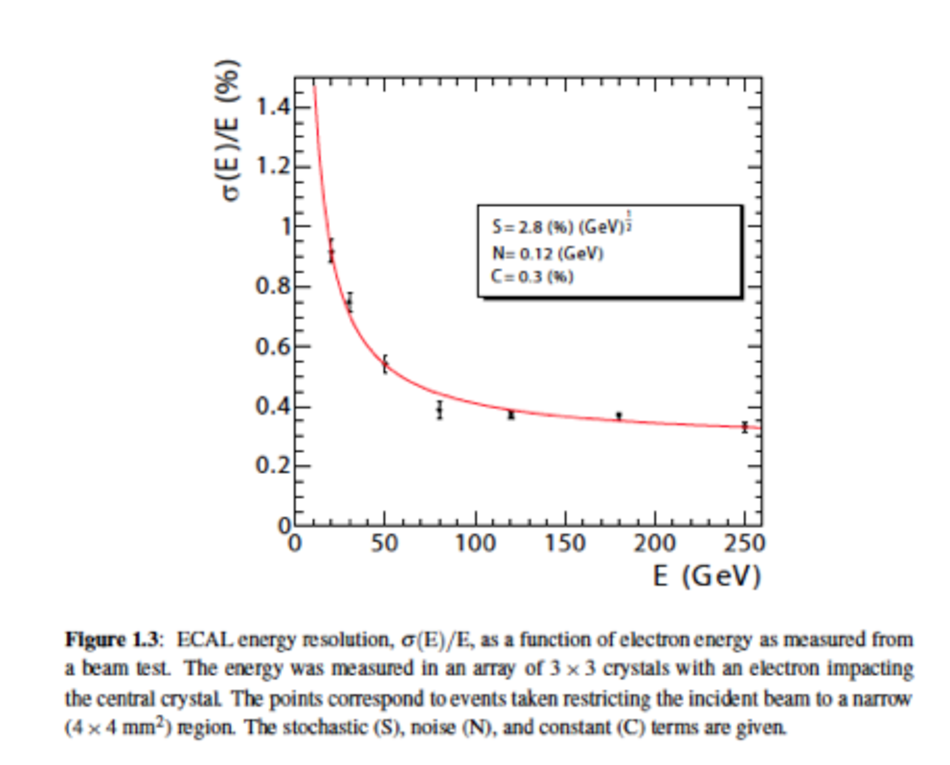
\includegraphics[scale=0.5]{./calorimetry/Pictures/fig9.pdf}
\caption{A figure stolen from JINST 3 S08004 showing the fractional resolution of the CMS barrel electromagnetic calorimeter as measured with electrons as a function of electron energy.}
\label{fig:cal8}
\end{figure}

\;

\section{read}

\;
$ \cdot \:$ Section 27.4 \url{http://pdg.lbl.gov/2011/reviews/rpp2011-rev-passage-particles-matter.pdf}

\;
\noindent
$ \cdot \:$  Section 28.9  \url{http://pdg.lbl.gov/2011/reviews/rpp2011-rev-particle-detectors-accel.pdf}

\;
\noindent
$ \cdot \:$  \url{http://journals.aps.org/rmp/abstract/10.1103/RevModPhys.75.1243}

\;
\noindent
$ \cdot \:$ \url{http://microcosm.web.cern.ch/microcosm/LHCGame/LHCGame.html}


\;
\noindent
$\cdot \:$ \url{http://www.sciencedirect.com/science/article/pii/S0168900211005572}

\;
\noindent
$\cdot \:$ \url{http://www.sciencedirect.com/science/article/pii/S0168900211019851}

\;
\noindent
$\cdot \:$ \url{http://www.sciencedirect.com/science/journal/01689002/666}

\;
\noindent
$\cdot \:$ \url{http://link.springer.com/article/10.1140$%$2Fepjc$%$2Fs10052-008-0573-yurl}

\;
\noindent
$\cdot \:$ \url{http://link.springer.com/article/10.1140$%$2Fepjc$%$2Fs10052-009-0959-5}

\;
\noindent
$\cdot \:$ \url{http://www.hamamatsu.com/resources/pdf/etd/PMT_handbook_v3aE.pdf}


%----------------------------------------------------------------------------------------
%	CHAPTER 7
%----------------------------------------------------------------------------------------
\chapterimage{Pictures/chapter_head_2.pdf} % Chapter heading image
\chapter{Trackers}

\section{Trackers}\index{EP}

this is not ported yet





%----------------------------------------------------------------------------------------
%	CHAPTER 8
%----------------------------------------------------------------------------------------
\chapterimage{Pictures/chapter_head_2.pdf} % Chapter heading image
\chapter{Particle Identification}
\section{Overview}\index{EP}
Now that we know how the basic elements of a particle physics detector work, let's see how we can use them to identify which types of particles produce which signals in our detector.  We will consider specifically the CMS detector, but virtually all collider detectors use similar identification criteria.
\newpage \noindent
Consider the following slice of the CMS detector as viewed in the r-$\phi$ plane: 
\begin{figure}[h]
\centering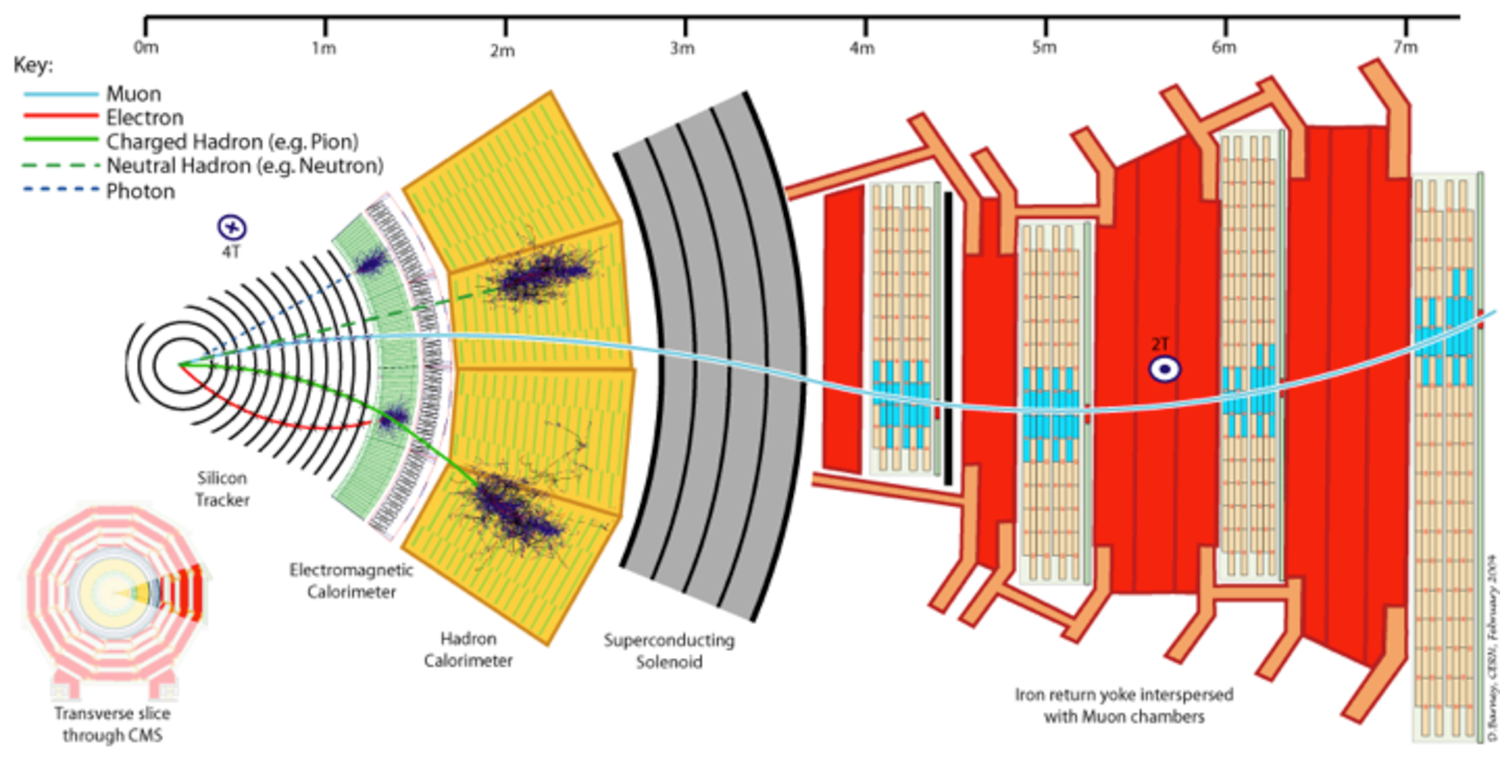
\includegraphics[scale=0.6]{./particleID/Pictures/fig1.pdf}
\caption{A slice of the CMS detector as viewed in the r-$\phi$ plane with typical signals produced by various types of particles. }
\label{fig:pdgdedx}
\end{figure} 
\\*
The collision point in the figure above is indicated by the convergence of the solid red, green, and blue lines and the dashed green and blue lines.  These represent particles created at a common point when a collision occurs.  Outward from the collision point, we have the silicon tracker, the electromagnetic calorimeter, the hadronic calorimeter, the solenoid magnet, and the muon trackers embedded in the ``return iron'' for the magnet (as you know, magnetic field lines must form closed loops. They cannot have a beginning or an end, until we discover the mythical magnetic monopole. The magnetic field lines that form the field inside the magnet must continue out one end, loop around, and come back to come in the other end. The ``return yoke'', made of iron, guides these field lines so that they do not interfere with the detector electronics).  
\\
\\
\noindent
Let's see how we can use the information from these detectors to identify particles.
\section{Photons}
In the figure, the photon is indicated by the dashed blue line.  Photons are electrically neutral so they do not produce a signal in any of the trackers.  Because they can interact with nuclei in the material via the long range electromagnetic interaction of pair production, they shower quickly upon impact, and the shower is almost completely contained in the EM calorimeter.
\section{Electrons}
In the figure, the electron is indicated by the solid red line.  Their signature is similar to that of a photon (although their initiating interaction is bremsstrahlung, not pair production), but there is an associated charged track.
\section{Muons}
In the figure, the muon is indicated by the solid blue line. Muons are charged and so they produce a track in the inner tracker. Muons predominantly loose energy by exciting or ionizing the electrons in the material.  Because of this, they lose energy slowly. They can pass through the calorimeters, losing only about a GeV of energy.  They are the only charged particle that can do this.  Tracking chambers (gas-based) outside the calorimeters, embedded in the return yoke, are used to indicate a penetrating particle.
\section{Hadrons}
In the figure, a charged hadron is indicated by the solid green line and a neutral hadron is indicated by the dashed green line. Hadrons interact with nuclei via the short-range strong force (QCD) interaction. Therefore, their shower will typically start deeper into the calorimeter and it will take more material to completely convert the kinetic energy of the hadron into energy of the material. The shower is needs the thicker combined electromagnetic and hadronic calorimeter to contain it. Charged and neutral hadrons are distinguished by the presence of a track in the tracker.
\section{Event displays}
While for physics results, complex computer algorithms are used to find the particles, the human mind also has very powerful identification capabilities.  Physicists use event displays to look at the information and identify particles ``by hand''.In the vast majority of the cases, when the human ``scanner'' and the computer algorithm disagree, the human is right.  It is important to verify computer algorithms and search for bugs by comparing the results from ``scanning''to the computer based results.
\\*
\\*
Typically two types of displays are used.  One has a cartoon of the detector with symbols to denote energy deposits.  The results from the computer identification algorithm are usually superimposed.  An example is shown below.  You can see the cartoon of the muon chambers in pink.  The tracks reconstructed in the tracker are shown as green lines.  Energies in the EM calorimeter are shown as red blobs and in the HAD calorimeter as blue blobs.  Their shape reflects the segmentation of the electrical readouts of the detector information.
\begin{figure}[h]
\centering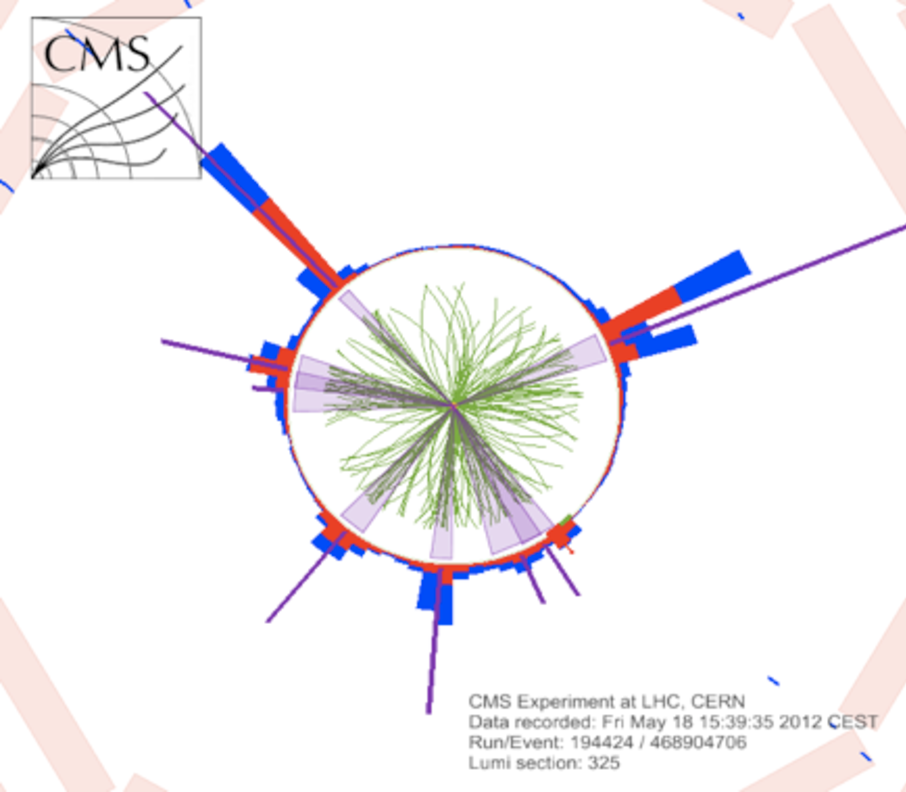
\includegraphics[scale=0.5]{./particleID/Pictures/fig2.pdf}
\caption{An event display from the CMS experiment}
\label{fig:pdgdedx}
\end{figure}
\\*
Another kind of event display is called a ``Lego'' plot (named after the Children's toy), and is the most common way of displaying calorimeter information.  This kind of display is a 3-D plot with two of the axes being the polar angle and the pseudorapidity, and the ``z'' axes being the energy deposited in the calorimeter at that location. Colors indicate which part of the energy was deposited in the electromagnetic and which in the hadronic calorimeter. An example is shown below, along with the corresponding regular display.
\begin{figure}[h]
\centering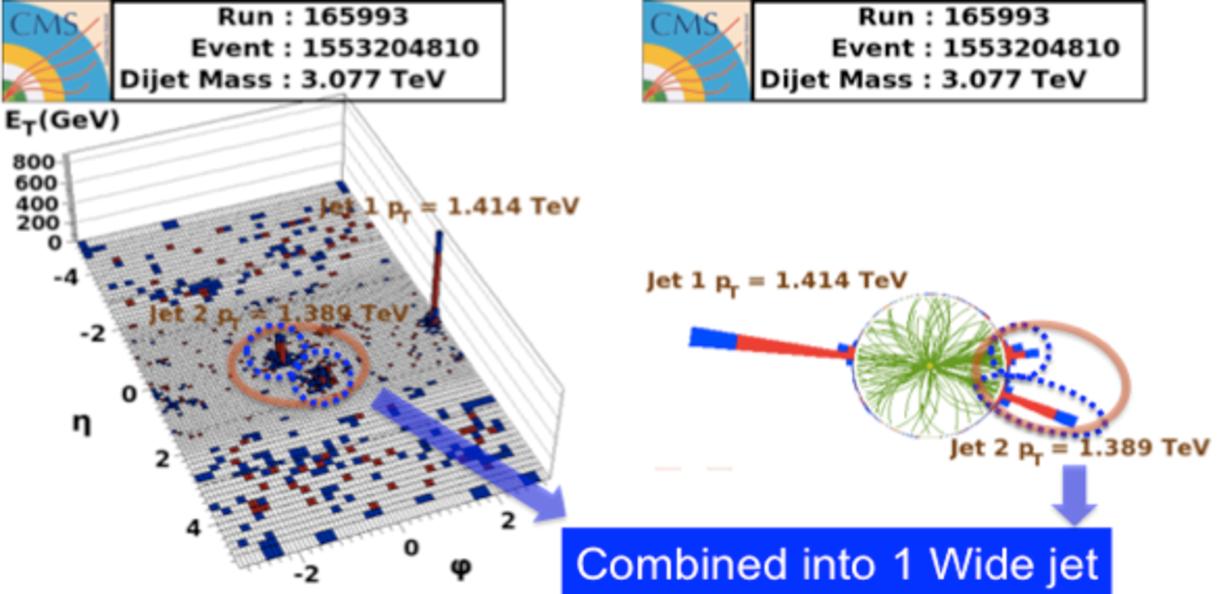
\includegraphics[scale=0.5]{./particleID/Pictures/fig3.pdf}
\caption{A lego display along wih the corresponding regular display of an event taken with the CMS detector.}
\label{fig:pdgdedx}
\end{figure}

\section{Neutrinos}
There is one particle that is so weakly interacting that does not produce a signal in our detector. However, we can infer their presence using conservation of momentum. The momentum of the beams is along the z-axis. This means that the total initial momentum can only be along the z direction, and the initial component of momentum transverse to the beam axis must be zero. By conservation of momentum, the final component of momentum transverse to the beam axis must also be zero.  So, if we sum the transverse momenta of all observed particles, the sum of the momenta of all unobserved particles must be equal in magnitude but opposite in direct to this, so that the sum is zero.  Usually this can be attributed to a single neutrino. The figure shown below shows the particles projected in the transverse plane. Since the observed momenta obviously cannot sum to zero, we infer that a neutrino was present in the event.
\begin{figure}[h]
\centering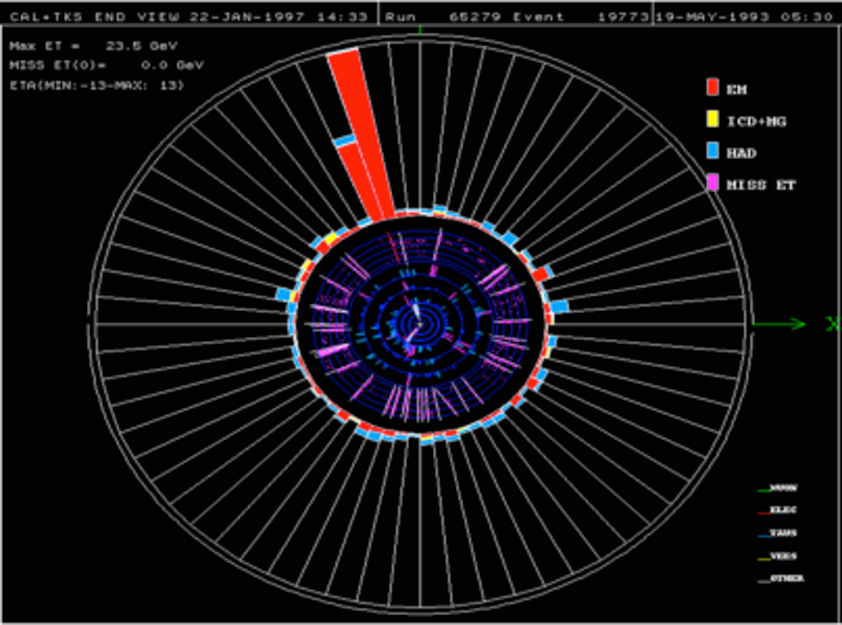
\includegraphics[scale=0.4]{./particleID/Pictures/fig4.pdf}
\caption{\small An event display from the D0 detector at the FNAL Tevatron.  The red blob represents energy in the EM calorimeter.  Since it has an associated track, it is identified as an electron. This is probably the decay of a W boson to an electron and a neutrino. The neutrino is assume to have a transverse momenta that is equal in magnitude and opposite in direction to the sum of the momenta of all other particles in the event.}
\label{fig:pdgdedx}
\end{figure}
\\*
This was, in fact, how Fermi discovered the neutrino - by considering conservation of momentum in certain radioactive decays of nuclei (beta decays). 
\newpage
\section{Quarks/Gluons (jets)}
As you may have noticed from the event displays shown above and from the one shown below, hadrons tend to come in clusters called ``jets''. These jets are the signatures of quarks and gluons, that ``fragment'' into a number of hadrons - typically 10 charged hadrons and 5 neutral, but with statistical fluctuations with the rms that occurs for any thing produced randomly that can counted ($\sqrt{N}$).
\\*
\\*
Generally, the individual momenta of the hadrons are not that interesting in our studies of forces and particles; what we really want to know is the momenta of the quarks and gluons that created them. To find this, we just have to figure out which hadrons came from the same ``parent'' particle and (by conservation of momentum), sum their momentum to get the parent momenta.
\\*
\noindent
However, because gluons can be radiated off quark or gluon jets, and the resulting jets are very close to each other (among other more fundamental but technical reasons), it is not trivial to figure out which hadrons belong together, which came from the same ``parent''.
\\*
To do this,``jet finding algorithms'' have been developed. The figure below shows how four different algorithms divided up the calorimeter energies into ``jets''.
\begin{figure}[h]
\centering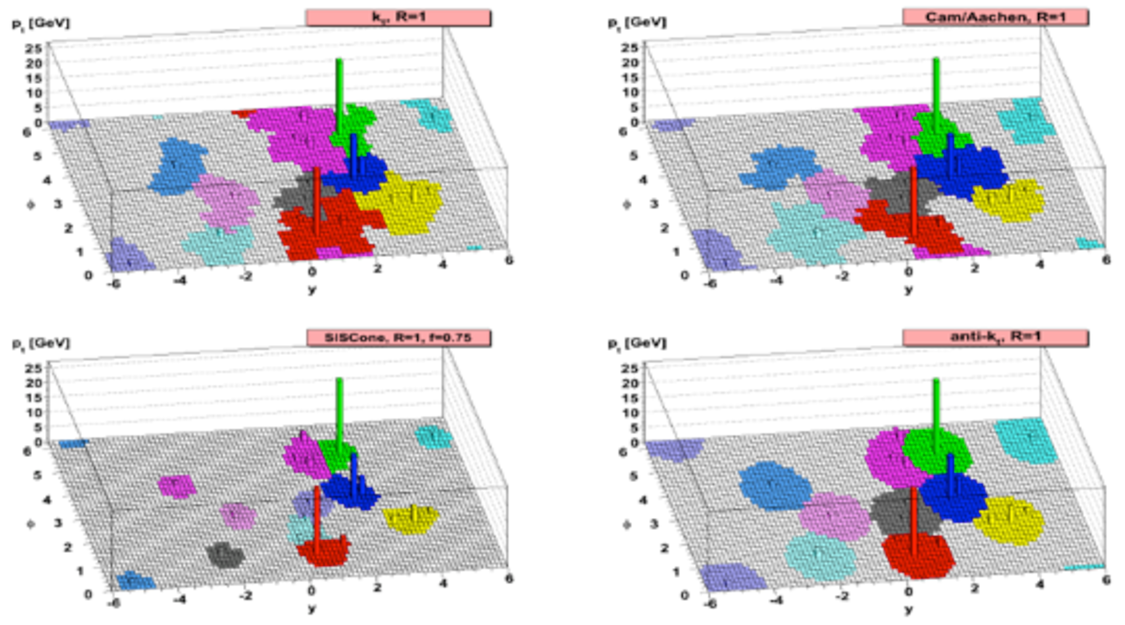
\includegraphics[scale=0.6]{./particleID/Pictures/fig5.pdf}
\end{figure}
\\*
\noindent
Let's look at one of these algorithms, which you will easily be able to imagine as code (and which clearly can not be handled any other way).  This algorithm is called the anti-$k_{T}$ algorithm (don't ask) with cone-parameter R. R is typically chosen to be 0.4.
\\*
\\*
$\cdot$ For all possible pairs of particles in an event (particle i and particle j), $d_{ij}$ = min(p$_{Ti}$$^{-2}$, p$_{Tj}$$^{-2}$)$\Delta\frac{R_{ij}^{2}}{R^{2}}$ where $R=\sqrt{(\Delta\phi)^{2}+(\Delta\eta)^{2}}$ and $\Delta\phi$ is the difference in azimuthal angles between the two particles and $\Delta\eta$ is the difference in their pseudorapidities.
\\
\noindent
$\cdot$ For each particle, calculate $d_{iB}$=$p_{T}^{-2}$

\noindent
$\cdot$ Take the minimum of all $d_{ij}s$ and $d_{iB}s$

\noindent
$\cdot$ If the smallest is a $d_{ij}$, combine them into a single particle by adding their 4-momenta, add this particle to the list of particles and remove the two individual particles.  Go back to the beginning.

\noindent 
$\cdot$ If it is a $d_{iB}$, call it a jet, remove the corresponding particle from the particle list, add it to the jet list, and go back to the beginning.

\noindent
$\cdot$ Stop when there are no particles left in the particle list.
\newpage
\noindent
\vspace{.2cm} 
\begin{minipage}{0.7\textwidth} 
\begin{framed}
%\vspace{.1cm}
\begin{exercise}
%\begin{frshaded}
%\fcolorbox{\bordercolor}{\backgroundcolor} 
{Look at the event displays found at xxx. For each event display, tell us what kind of particles you see}
\end{exercise}
%\end{frshaded}
%\vspace{.1cm}
\end{framed} 
\end{minipage}
\vspace{.2cm}
\\*
\vspace{.2cm} 
\begin{minipage}{0.7\textwidth} 
\begin{framed}
%\vspace{.1cm}
\begin{exercise}
%\begin{frshaded}
%\fcolorbox{\bordercolor}{\backgroundcolor} 
{The root file blablabla has particle 4-momenta for particles reconstructed for a bunch of events. Write code to cluster these into jets. Use the anti-$k_{T}$ cone algorithm with cone parameter 0.4. Make a histogram showing the $p_{T}$ spectra of the jets.}
\end{exercise}
%\end{frshaded}
%\vspace{.1cm}
\end{framed} 
\end{minipage}
\vspace{.2cm}

\section{Further Reading}
\noindent
$\cdot$ \url{http://www.sciencedirect.com/science/article/pii/S0168900211005419}


%----------------------------------------------------------------------------------------
%	CHAPTER 9
%----------------------------------------------------------------------------------------
\chapterimage{Pictures/chapter_head_2.pdf} % Chapter heading image
\chapter{The LHC Detectors}

\section{Disclaimer}\index{Disclaimer}

this is not ported yet





%----------------------------------------------------------------------------------------
%	CHAPTER 10
%----------------------------------------------------------------------------------------
\chapterimage{Pictures/chapter_head_2.pdf} % Chapter heading image
\chapter{Structure of the proton and proton-proton collisions}
\section{Cross section}\index{Cross Section}
Imagine a 2-D box in deep space, away from gravity, containing some number of large 2D disks.  If you threw a ball at the box, the probability of hitting a disks is related to the ratio of the cross sectional area of the box to the cross sectional area of the disks.  The cross sectional area of the disks is their 
``cross section'', often denoted ${\rm \sigma}$ and has units of area.  
If you look at a solid and imagine scattering particles off the nuclei inside them, it is similar.  Remember that solids are, after all, mostly empty space.  If you project all the nuclei into the 2D front face of the solid, you have our 2-D box.  The cross section area of a nuclei is measured in ${\rm fm^{2}}$.  
For low energy scattering by the strong force, since the strong force only has a very short range, and interactions can only happen if the ball virtually touches the nucleus, this is a good approximation.  A unit commonly used in the barn, which is \(10^{28} m^{2}\).  Nuclear �cross sections� are around 80 mbarns.  For forces with a longer range, such as E\&M, we define instead an �effective� area.  See any introductory book on particle physics for a more precise definition.

What if instead you threw a steady stream of balls at the box and wanted to calculate the rate at which balls hit beads and are deflected?  Also, as you can imagine, in realistic beams the projectiles do not march single file.  You should imagine them moving in a cylinder with some cross section, like Figure ~\ref{fig:beam}.

\begin{figure}[h]
\centering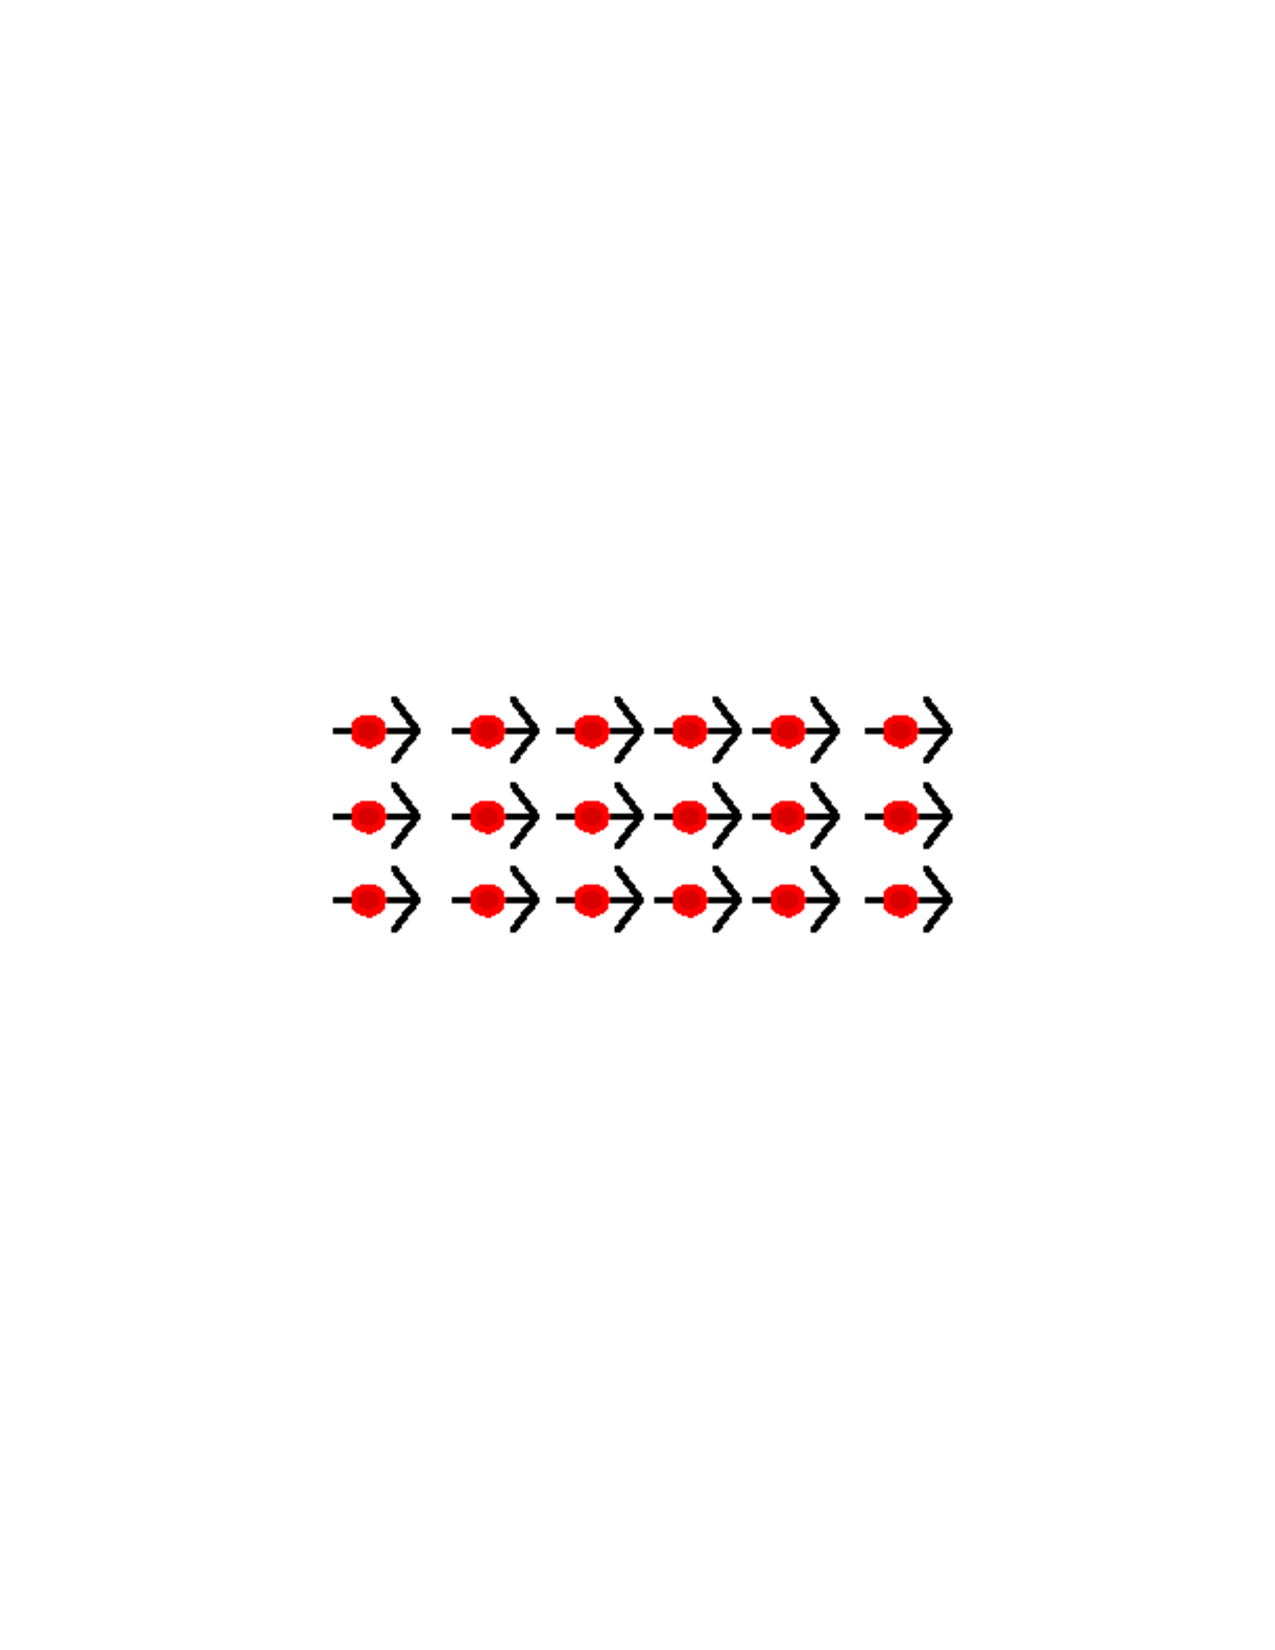
\includegraphics[scale=0.5]{./protonprotoncollisions/Pictures/beam.pdf}
\caption{cartoon of a beam of particles}
\label{fig:beam}
\end{figure}



If the number of balls in the beam per unit area is na, and the velocity of the balls is v,  then the number of balls reaching the target per second is

\begin{equation}\Phi = n_{a}v\end{equation}

and \(\Phi\) is called the flux.  What are the units of \(\Phi\)?

The number of scatters per second is then

\begin{equation}\frac{dN}{dt}=\Phi \sigma
\end{equation}

(check that the units work).

Now, you may ask what happens in a collider?  Well, it is just the same.  You can always move to a frame where one of the protons is at rest, do the calculation there, and move back.  We will see in the next section why our calculation of the cross section does not depend on the frame in which it is calculated.

\section{s, t, u, and q squared}\index{s, t, u, and q squared}

As we have seen, in relativity, there are ``invariants'' that will be 
measured to be the same by all observers, regardless of 
their frame and relative motion of the particle.  One of these is the length of a particle's 
4-momentum, which is its mass.  In collisions, there are a few of these variables that are important, as cross sections calculated from the standard model must be functions only of these variables and numeric factors.  The most important ones were unimaginably given the names s, t, u and Q2.  Imagine some kind of reaction (could be photon exchange, gluon exchanged, Z exchange etc) where two particles a and b come in and two particles c and d come out  (called a 2-to-2 reaction, figure ~\ref{fig:twototwo}).

\begin{figure}[h]
\centering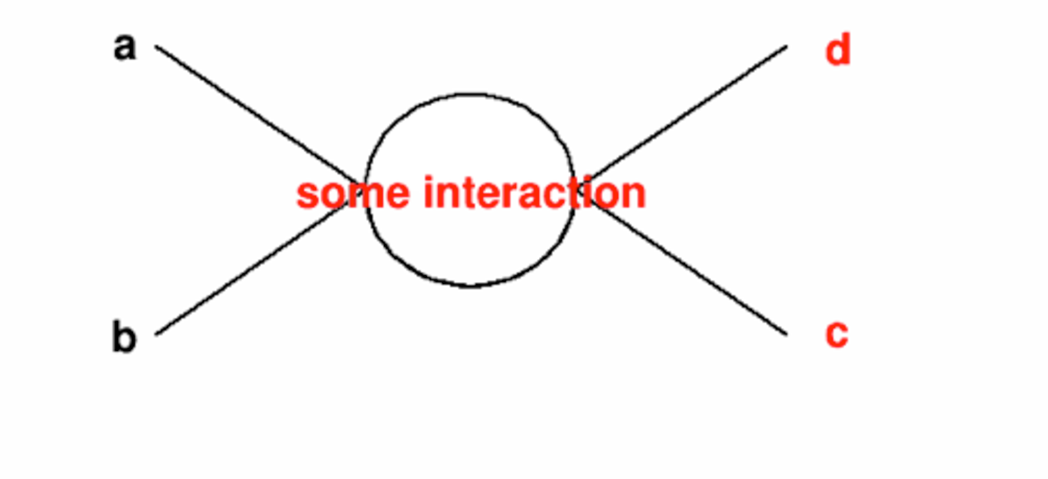
\includegraphics[scale=0.5]{./protonprotoncollisions/Pictures/fig1.pdf}
\caption{generic interaction of 2 particles going to 2 particles}
\label{fig:twototwo}
\end{figure}

If \(p_{a}\) is the 4-momentum of particle A and the 4-momenta of the other particles are named similarly, then

\begin{equation}s=(p_{a}+p_{b})^{2}\end{equation}
\begin{equation}t=(p_{a}-p_{c})^{2}\end{equation}
\begin{equation}u=(p_{a}-p_{d})^{2}\end{equation}

Remember: the square here means dot product, and the dot product of a 4-vector is the square root of the product of the first components (time-like components) minus the dot product of the 3D part of the 4 vector.  So s, t, u are a bit like a mass.  All these variables have units of \(GeV^{2}\).

Another important variable is \(Q^{2}\).  This can be u for some interactions and s for others.  It is the �mass� of the virtual particle that is exchanged in the interaction (the photon, W, Z, etc).  
Now, you may say: but the photon is massless!  But, that is only if it is observable.  The photon can be ``off-shell'' as long as it is unobservable (for times short compared to that set by the uncertainty principle, using M as E), meaning that it has a non-zero mass.  You will learn more about this when you study quantum mechanics.

It can be shown in quantum field theory that, in the frame where the 4-momentum of particles a and b are equal but opposite and have high enough energy that we can neglect their mass, that the cross section can be calculated from the physics of the standard model using a simple formula

\begin{equation}
\frac{d?}{d\Omega} = \frac{1}{64\Pi^{2}s}\frac{P_{f}}{P_{i}}|M|^{2}
\end{equation}

where \(p_{f}\) is the magnitude of the 3-momenta of either particle c or d (why doesn�t it matter which?) and pi is that of either a or b.  What will the ratio of pf to pi be if particles c and d both have momenta large compared to their mass as well?

\(|M|^{2}\)  is a factor called the �matrix element� which is calculated from the standard model and must be a function of s, t, u and numeric factors.

\section{What is in a Proton}\index{What is in a Proton}
You may have been taught that a proton contains two up quarks and a down quark.  This is not true.  In fact, only half the momentum of a proton is carried by quarks.  What carries the other half?  This is a complicated question.  Roughly, we can say that about half the momentum is carried by the up and down quarks, and about half by gluons.  One of the goals of nuclear physics is to understand how the momentum distribution of the proton is divided amoung the protons constituents.  The �Parton Distribution Functions� or PDFs give the probability of finding a �parton� (a constituent of the proton, like a quark or gluon) with a fraction of the proton momentum x.  When you sum over all partons and all x, you should get 1 (when you add them all together, you have the whole momentum of the proton).  Figure ~\ref{fig:pdfpdf} shows results from measurements.

\begin{figure}[h]
\centering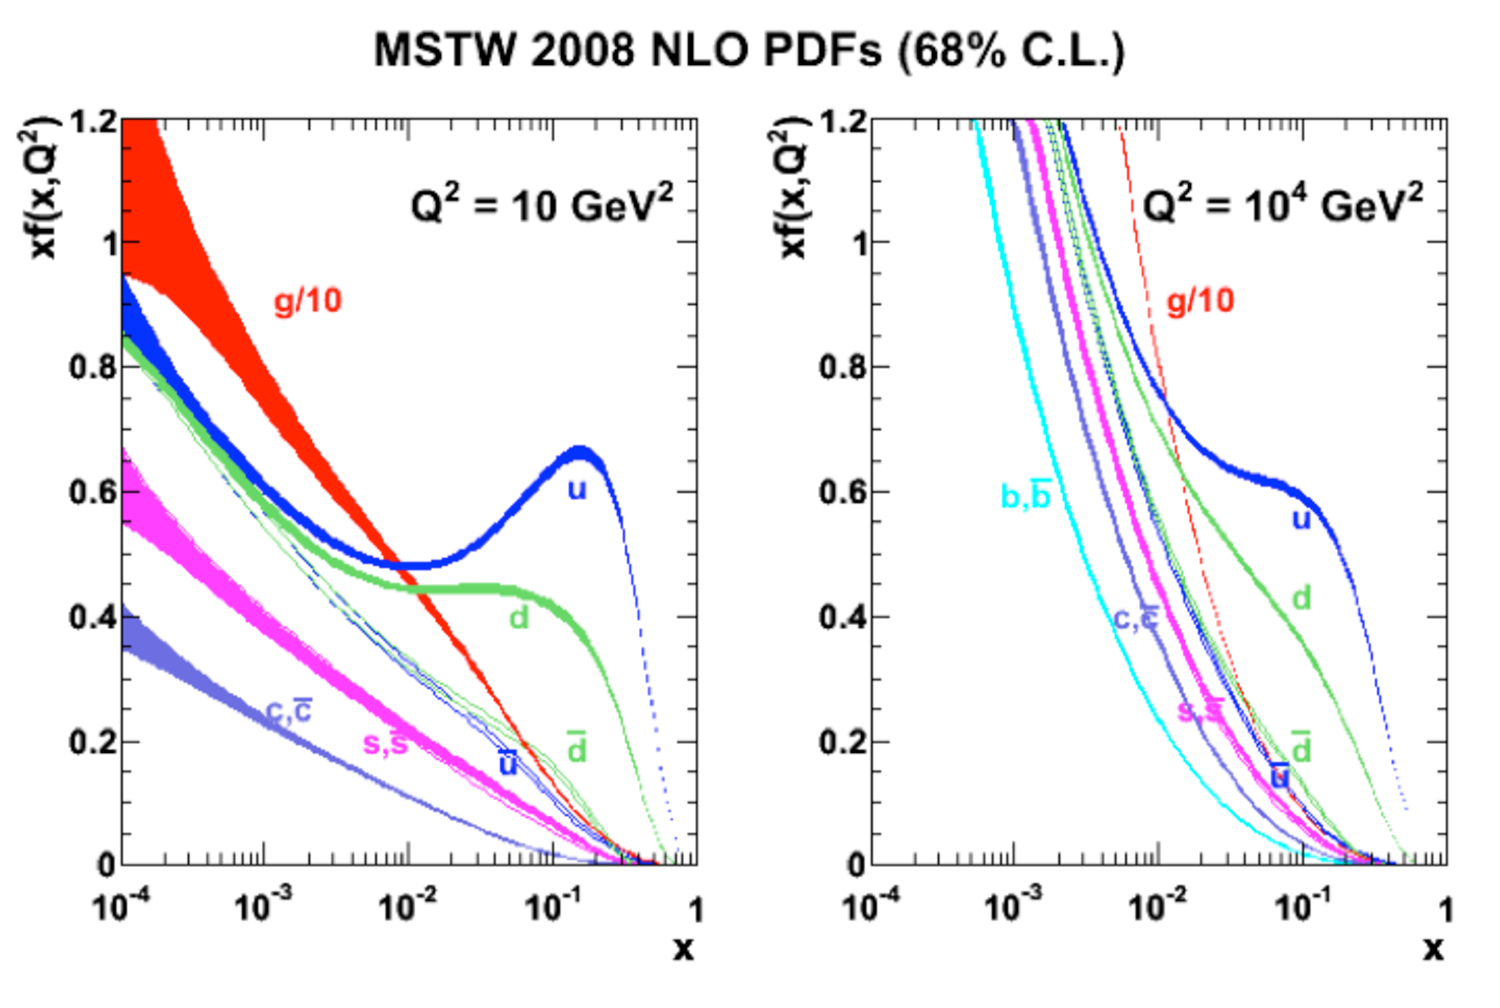
\includegraphics[scale=0.5]{./protonprotoncollisions/Pictures/fig2.pdf}
\caption{probability of finding a parton that has a fraction x of the proton momentum times x for different parton flavors}
\label{fig:pdfpdf}
\end{figure}
However, the truth is, if you look inside a proton, what you see depends on how closely you look. The closer you look, the more detail you see.  Interactions with large \(Q^{2}\) look more closely that those that don�t (think about the uncertainty principal and it may help you understand).  That is why there are two figures in the picture shown above.  One shows what the proton looks like if you probe it with a virtual particle with low \(Q^{2}\) and the other shows it with a higher \(Q^{2}\) probe.

How do we do this?  Most of the information comes from ``fixed target experiments'', which collide a beam of particles with some kind of target, perhaps copper or something else that won't melt in a high radiation environment, and from the ``HERA'' collider in Hamburg Germany, which collides electrons with protons.

Imagine two possible beams in a fixed target experiment: muons and neutrinos.  Muons will interact with the up and down quarks (and other quarks) in the  proton via photons, more with the up quarks than with the down quarks due to their larger electric charge.  If we switch to a different target which has a different ratio of neutrons to protons, we get a different ratio of up and down quarks and different scattering rates.  Neutrinos interact with the protons and neutrons via the weak force, mostly the Z boson.  These also interact differently with up and down quarks, but in a different way.  Groups of theorists, such as �MRST� and �CTEQ� take all this data and untangle from it the �parton distribution functions�.  Note that neither type of beam interacts directly with gluons and therefore there is larger uncertainty on this part of the PDF than that of the quarks.

\section{Calculation of a cross section in proton proton collisions}\index{Calculation of a cross section in proton proton collisions}

In a proton-proton collision, the particles and b are partons in the proton.  For a given final state (particles c and d), there can be a variety of different initial states that can occur.  For example, a Z boson can be created when an up quark annihilates with an anti-up quark or it can be created when an down quark annihilates with an anti-down quark.  It is like our bean has different kinds of balls that have a different effective cross section to interact with the target.  How can we calculate the total cross section for any two partons in the proton to go to a Z and then into, say an electron-positron pair?  We need to integrate over all possible initial states:

\begin{equation}
\sigma = \Sigma \int{dx_a dx_b \sigma[q(x_a)\bar{q(x_b)}+q(x_b)\bar{q(x_a)}]}
\end{equation}

where the q's represent the PDFs for the quarks.

\section{What happens when two protons collide?}\index{What happens when two protons collide?}
First remember that quantum mechanics applies.  We can calculate the probability of certain kinds of interactions, but we cannot predict event by event which one will occur.  The pie chart shown in Figure ~\ref{fig:productionprobs} the fraction of collisions that result in different types of interactions.

\begin{figure}[h]
\centering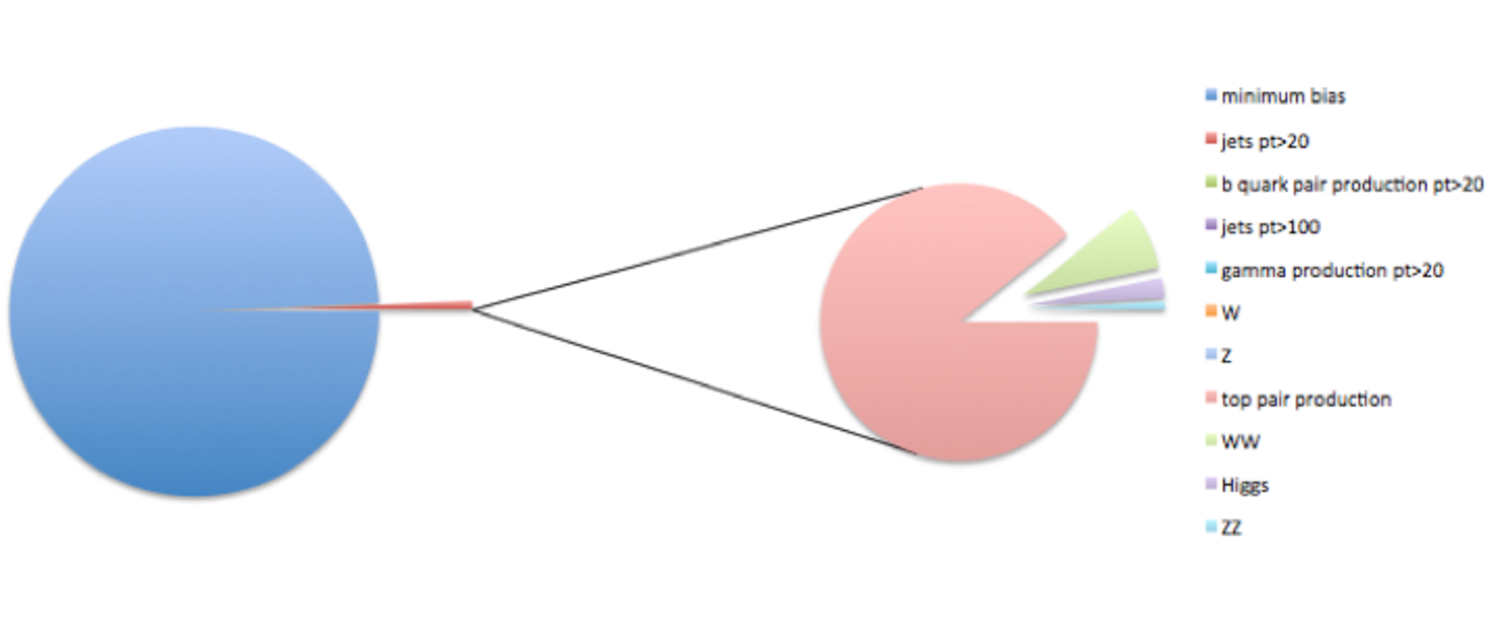
\includegraphics[scale=0.5]{./protonprotoncollisions/Pictures/fig3.pdf}
\caption{Pie chart showing relative probabilities of different types of interactions in proton-proton collisions}
\label{fig:productionprobs}
\end{figure}
Another way to look at this is using the cross sections, shown in Figures ~\ref{fig:lhcsigma1} and  ~\ref{fig:lhcsigma2}.

\begin{figure}[h]
\centering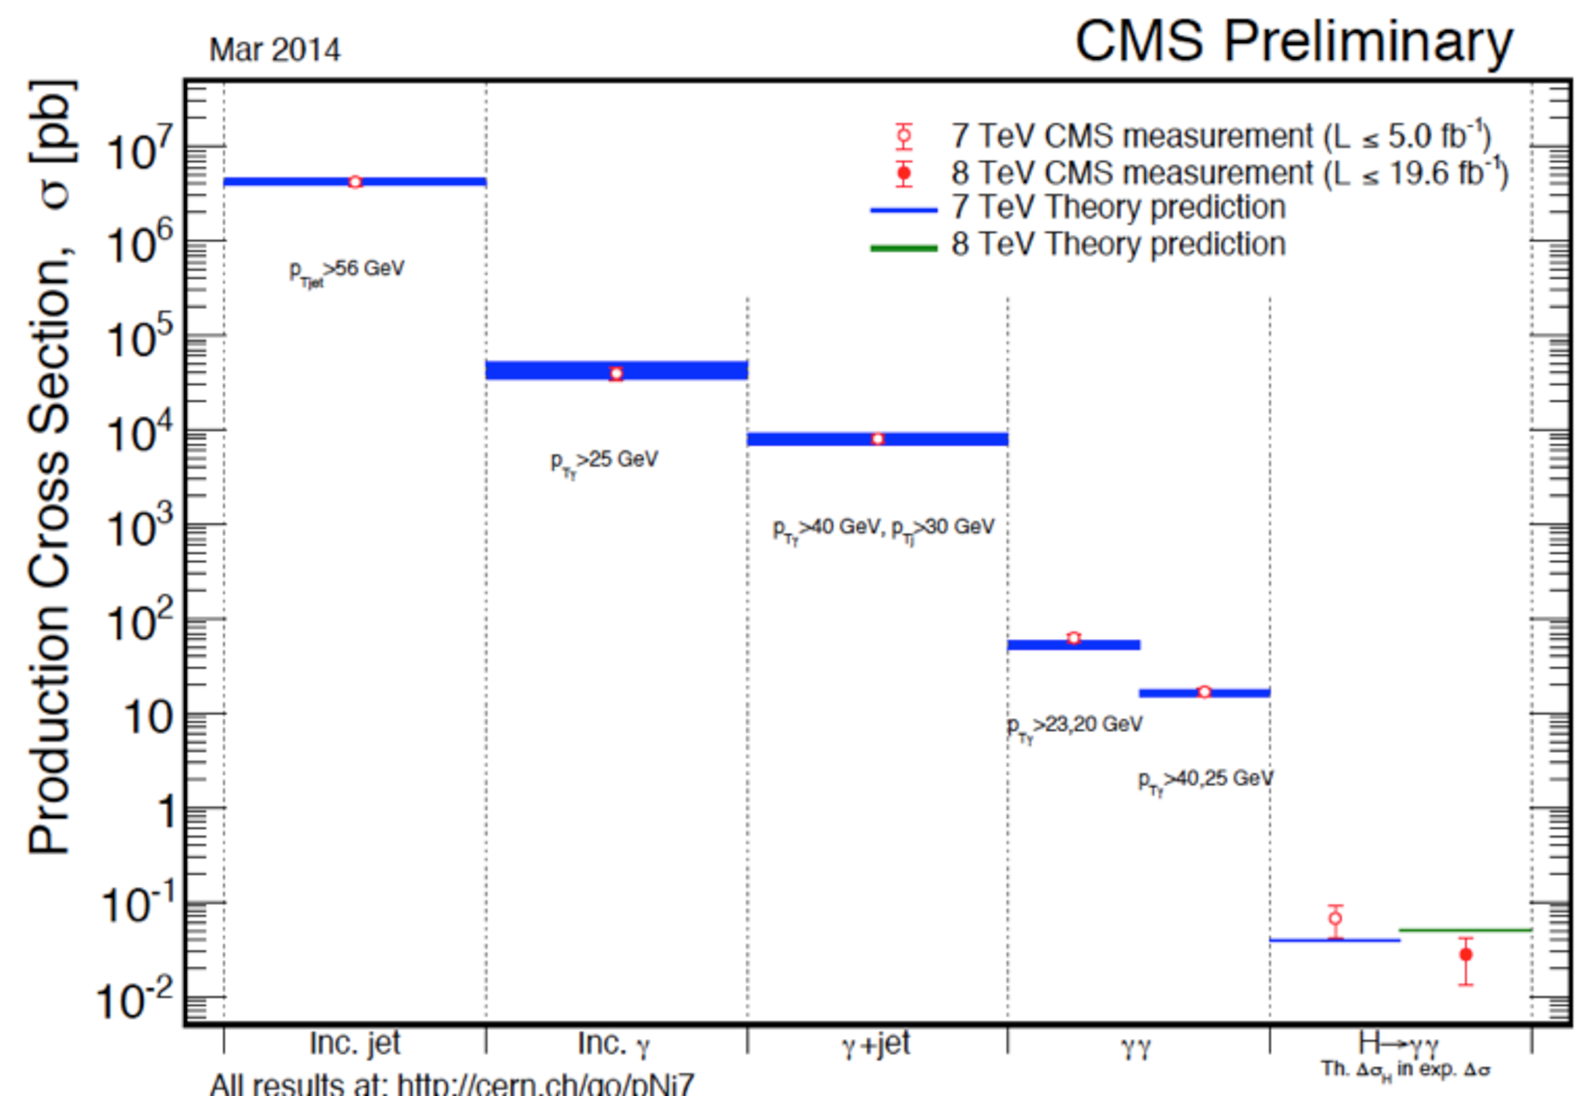
\includegraphics[scale=0.5]{./protonprotoncollisions/Pictures/fig4.pdf}
\caption{Cross sections for production of various combinations of particles at the LHC for a center of mass energy ${\rm Q^@}$ of 8 TeV}
\label{fig:lhcsigma1}
\end{figure}
\begin{figure}[h]
\centering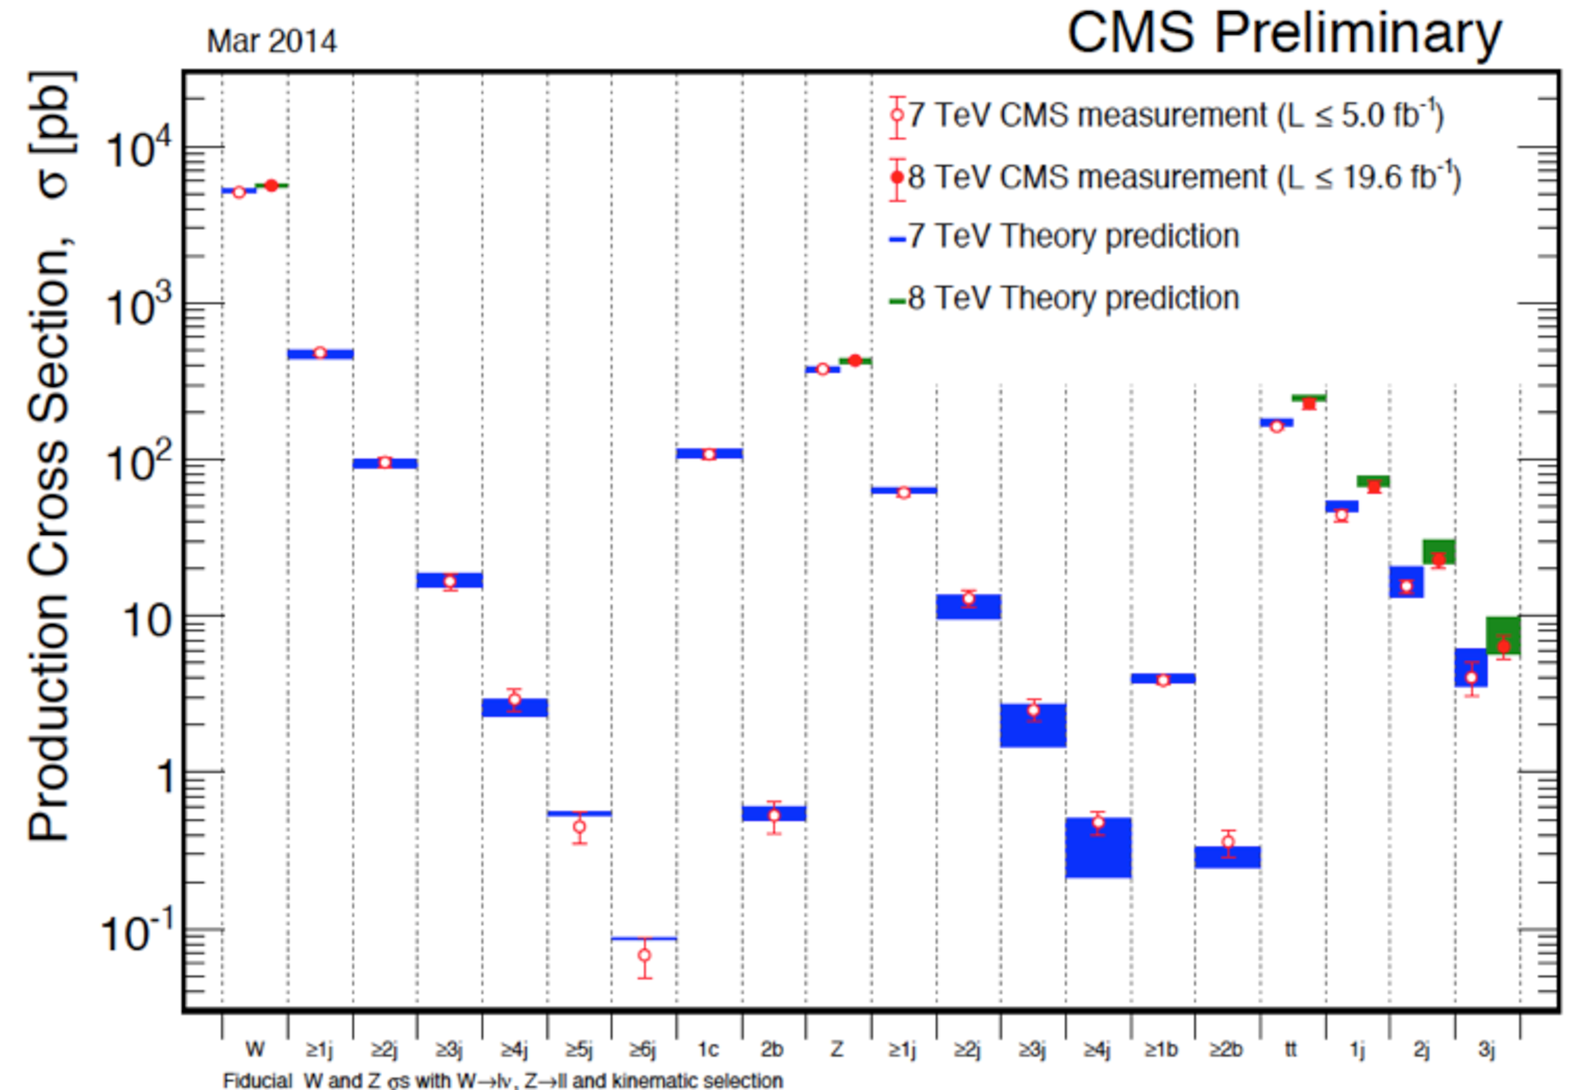
\includegraphics[scale=0.5]{./protonprotoncollisions/Pictures/fig5.pdf}
\caption{Cross sections for production of various combinations of particles at the LHC for a center of mass energy ${\rm Q^2}$ of 8 TeV.}
\label{fig:lhcsigma2}
\end{figure}


What are these things?

\section{Minimum bias interaction}\index{Minimum bias interaction}

The most common thing to occur is that a small amount of momentum is exchanged between the proton, in the form of gluons, or color-neutral combinations of gluons, resulting in a few pions being spit out.  A cartoon might look Figure ~\ref{fig:minbias}.

\begin{figure}[h]
\centering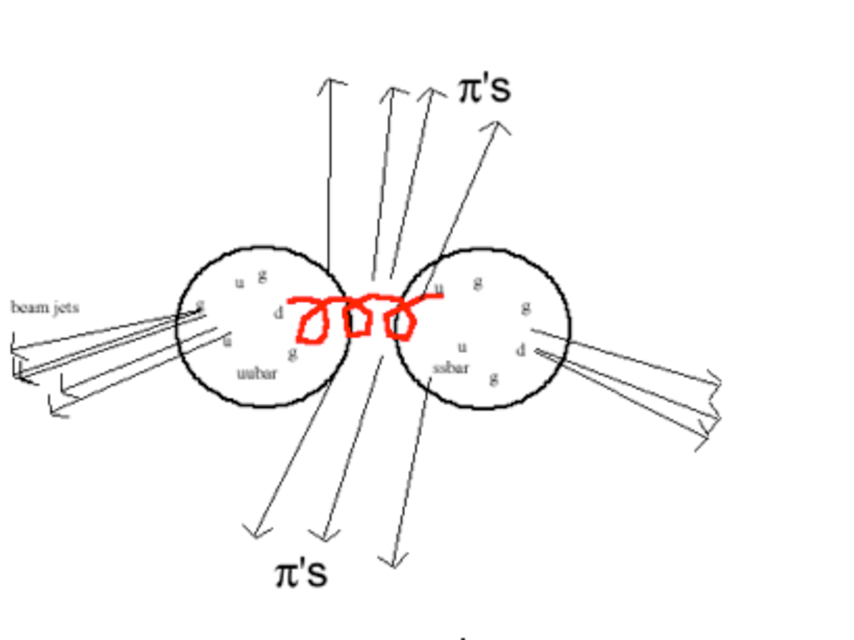
\includegraphics[scale=0.5]{./protonprotoncollisions/Pictures/fig6.pdf}
\caption{carton of a minimum bias interaction}
\label{fig:minbias}
\end{figure}

\section{Jets}\index{Jets}

The strong force is strong.  Therefore one of the most common things to make in proton-proton collisions are quarks and gluons.  As we know, these particles appear as jets of hadrons in our detector.  Some Feynman diagrams for this process are shown in Figure \ref{fig:jetfeyn}.  Typical event displays for this kind of event is shown in Figures \ref{fig:jetdis1} and \ref{fig:jetdis2}.

\begin{figure}[h]
\centering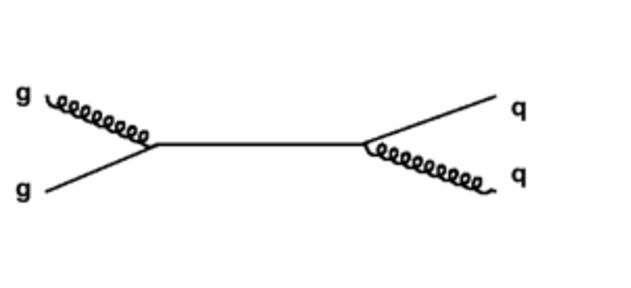
\includegraphics[scale=0.5]{./protonprotoncollisions/Pictures/fig8.pdf}
\centering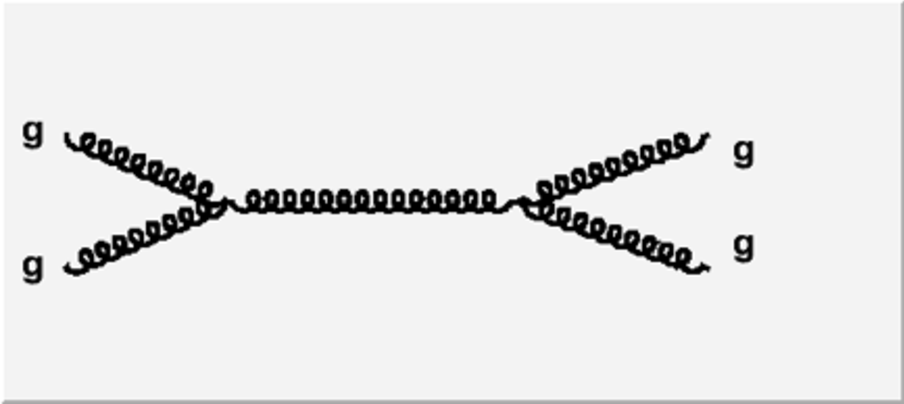
\includegraphics[scale=0.5]{./protonprotoncollisions/Pictures/fig7.pdf}
\caption{Feynman diagrams for productions of jets.}
\label{fig:jetfeyn}
\end{figure}


\begin{figure}[h]
\centering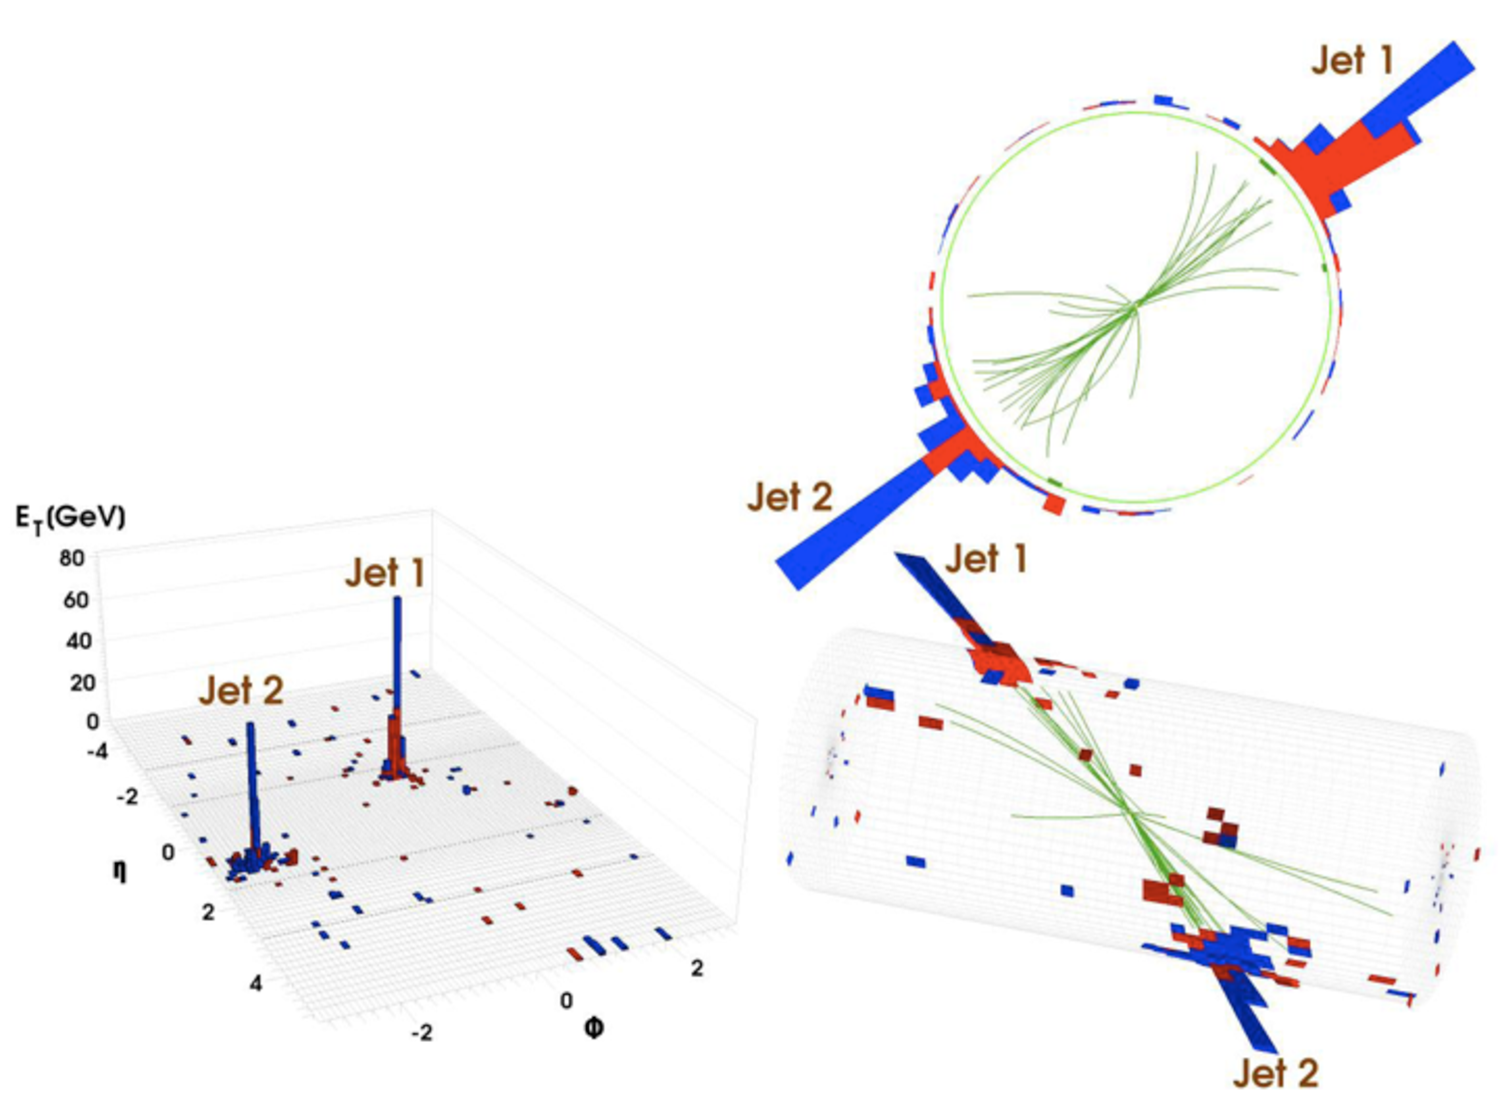
\includegraphics[scale=0.5]{./protonprotoncollisions/Pictures/fig9.pdf}
\caption{event display for jet production}
\label{fig:jetdis1}
\end{figure}

\begin{figure}[h]
\centering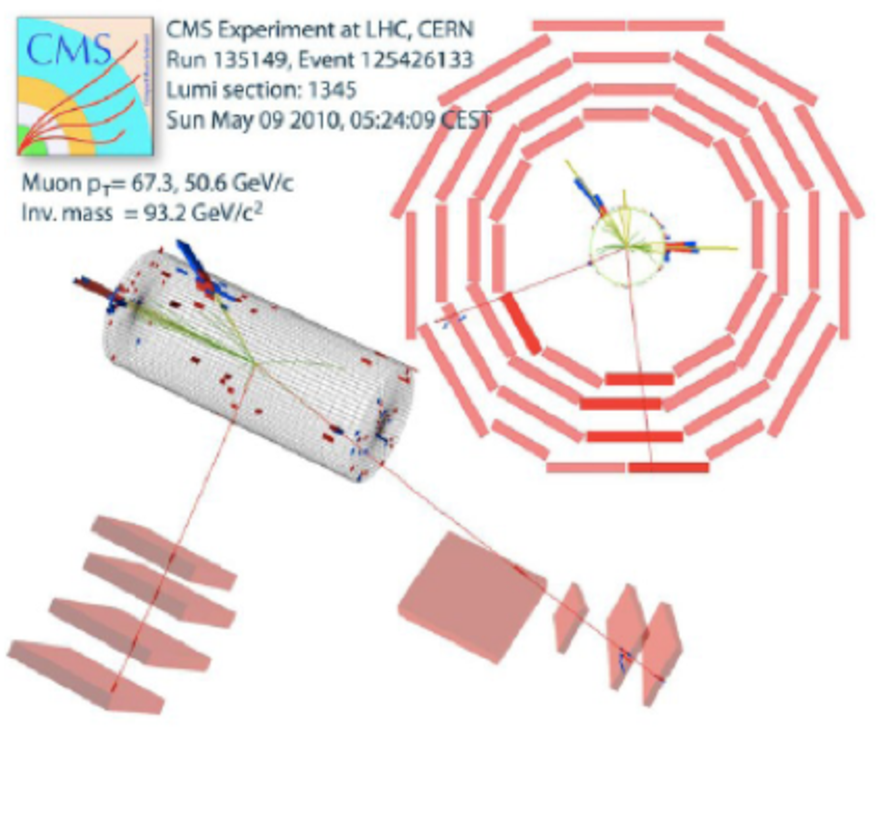
\includegraphics[scale=0.5]{./protonprotoncollisions/Pictures/fig10.pdf}
\caption{event display for jet production}
\label{fig:jetdis2}
\end{figure}

\section{W and Z production}\index{wz}

You can also make the carriers of the weak force, the W and Z bosons.  Some Feynman diagrams are shown in Figure ~\ref{fig:wzfeyn}.
An event display is shown in Figure ~\ref{fig:wzevent}.

\begin{figure}[h]
\centering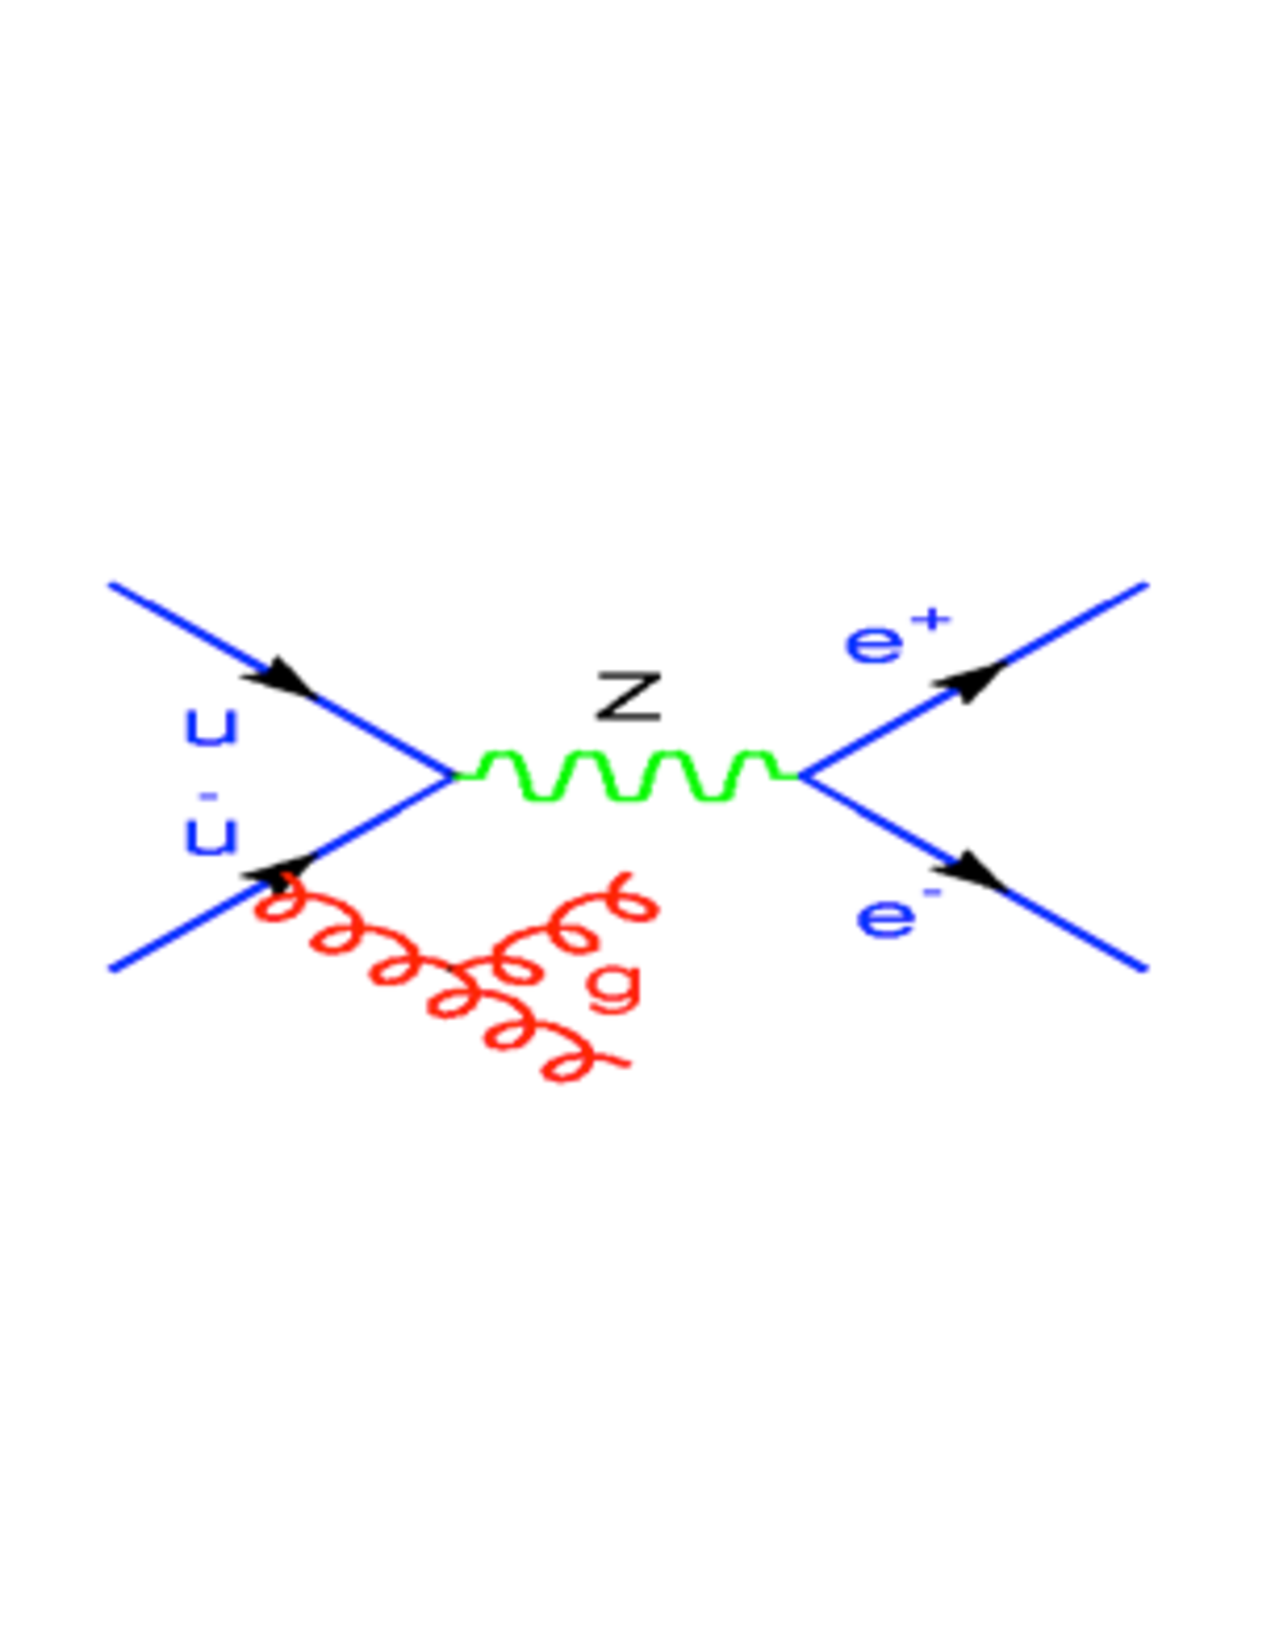
\includegraphics[scale=0.2]{./protonprotoncollisions/Pictures/wz1.pdf}
\centering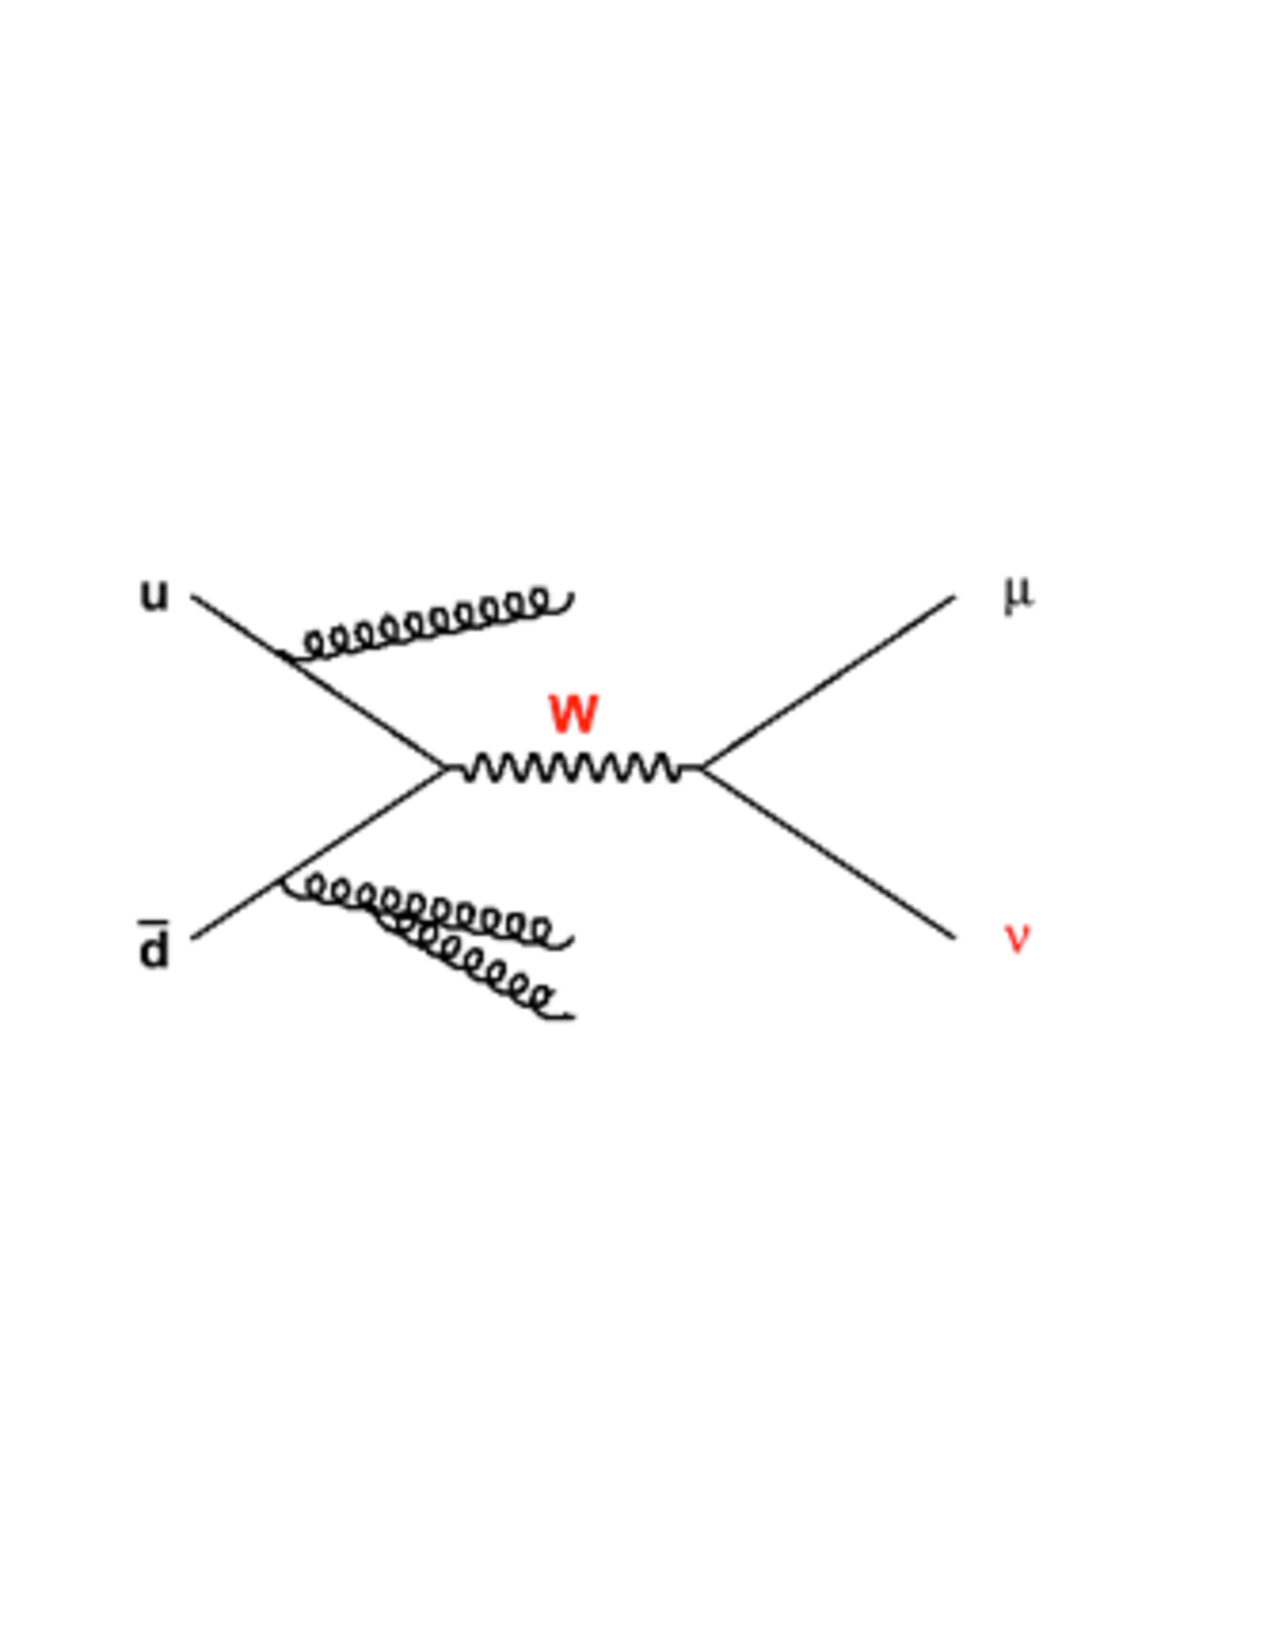
\includegraphics[scale=0.2]{./protonprotoncollisions/Pictures/wz2.pdf}
\caption{Feynman diagrams for productions of W or Z bosons.}
\label{fig:wzfeyn}
\end{figure}


\begin{figure}[h]
\centering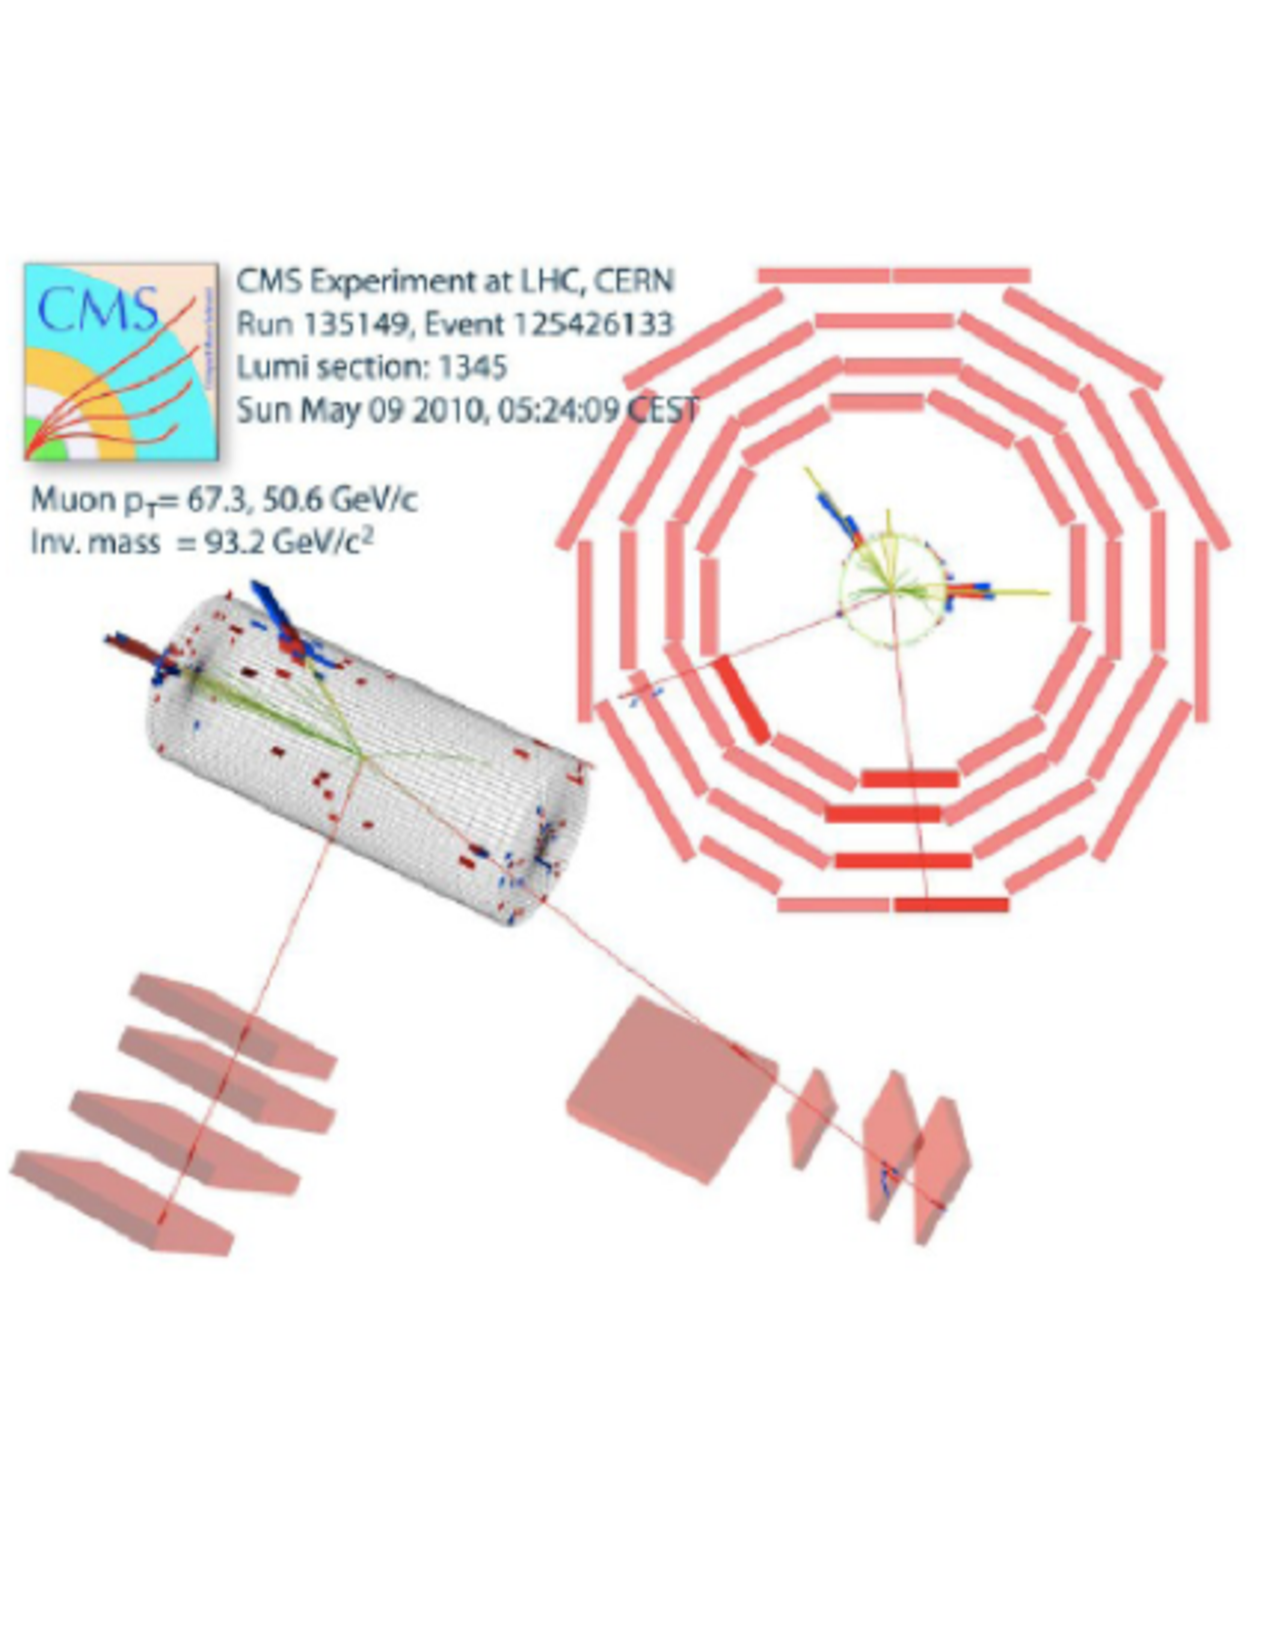
\includegraphics[scale=0.5]{./protonprotoncollisions/Pictures/wzevent.pdf}
\caption{Event display for a Z boson}
\label{fig:wzevent}
\end{figure}

\section{top production}\index{topprod}

You could also make the heaviest of the quarks, the top quark.  Most commonly, it is made with an anti-top.   The Feynman diagram is shown in Figure ~\ref{fig:topfeyn}, along with a pie chart showing the probabilities that the two tops in the events will decay to different final states containing particles stable on detector timescales.  A display of an event that could be top pair production is shown in Figure \ref{fig:topdisk}.

\begin{figure}[h]
\centering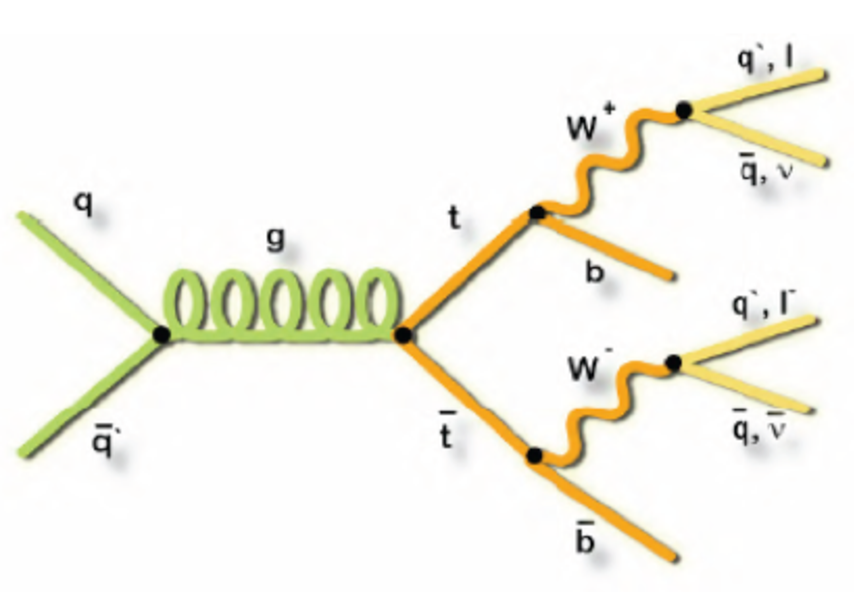
\includegraphics[scale=0.3]{./protonprotoncollisions/Pictures/fig11.pdf}
\centering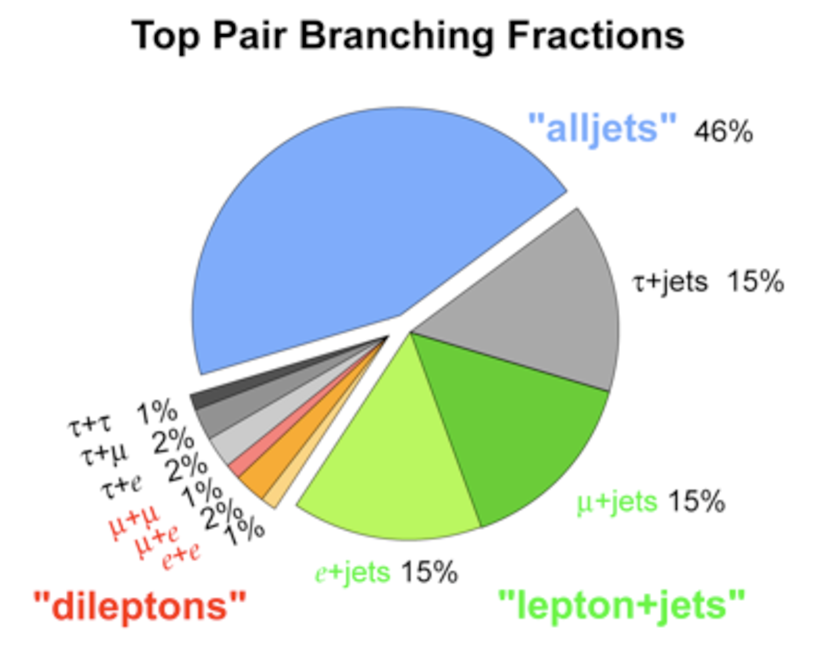
\includegraphics[scale=0.3]{./protonprotoncollisions/Pictures/fig12.pdf}
\caption{Feynman Diagram for top production and branching fraction for top to different final states}
\label{fig:topfeyn}
\end{figure}

\begin{figure}[h]
\centering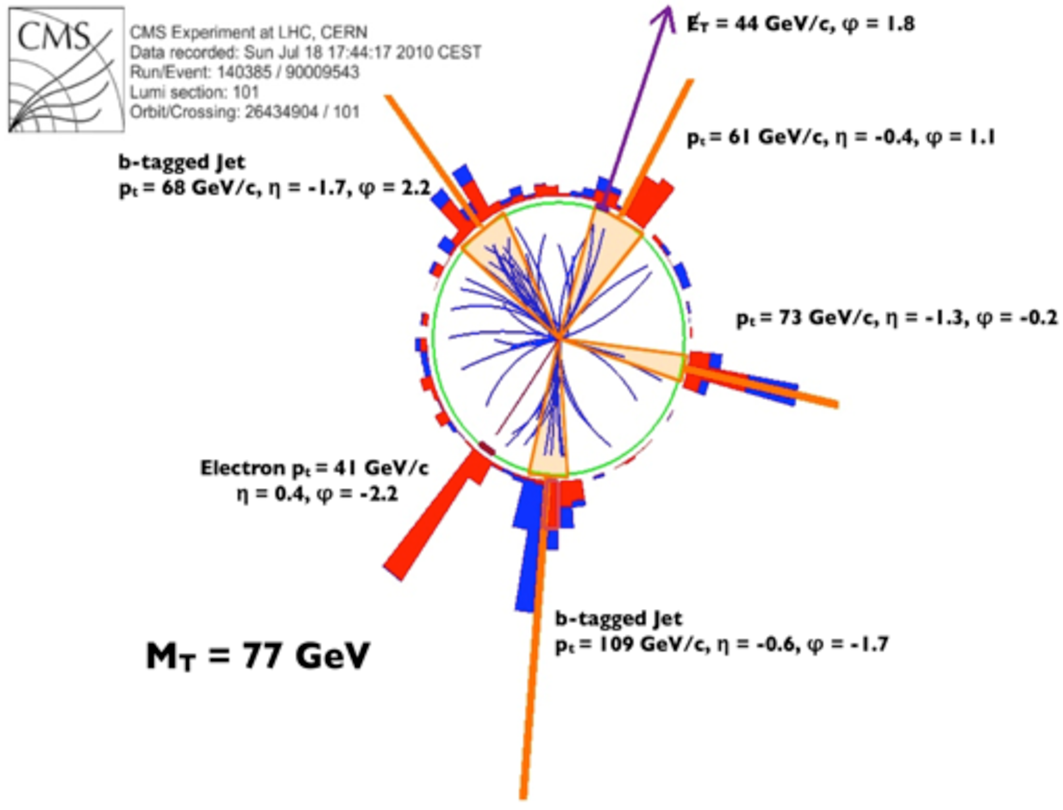
\includegraphics[scale=0.5]{./protonprotoncollisions/Pictures/fig13.pdf}
\caption{Event Display for top pair production}
\label{fig:topdisk}
\end{figure}

\section{Further Reading}\index{Further Reading}

\begin{itemize}
\item http://xxx.lanl.gov/abs/hep-ph/9606399
\item http://iopscience.iop.org/0034-4885/70/1/R02/
\item �Modern Particle Physics� by Mark Thomson
\item �Introduction to Elementary Particle Physics� by Alessandro Bettini
\end{itemize}


%----------------------------------------------------------------------------------------
%	CHAPTER 11
%----------------------------------------------------------------------------------------
\chapterimage{Pictures/chapter_head_2.pdf} % Chapter heading image
\chapter{Monte Carlos}

\section{Disclaimer}\index{Disclaimer}

this is not ported yet





%----------------------------------------------------------------------------------------
%	CHAPTER 12
%----------------------------------------------------------------------------------------
\chapterimage{Pictures/chapter_head_2.pdf} % Chapter heading image
\chapter{Higgs Discovery}

\section{higgs to four leptons}\index{higgs4l}

Please read http://arxiv.org/pdf/1312.5353.pdf





\section{Acknowledgements}
The authors would like to thank Fred Buchanan, Nirmarta Kaur, Victor Meszaros, and Yao Yao for help at every stage of the creation of this work.


\end{document}



%---------------------------------------------------------------------------------------------------------------------------------------------------------------------------

%------------------------------------------------

\section{Citation}\index{Citation}

This statement requires citation \cite{book_key}; this one is more specific \cite[122]{article_key}.

%------------------------------------------------

\section{Lists}\index{Lists}

Lists are useful to present information in a concise and/or ordered way\footnote{Footnote example...}.

\subsection{Numbered List}\index{Lists!Numbered List}

\begin{enumerate}
\item The first item
\item The second item
\item The third item
\end{enumerate}

\subsection{Bullet Points}\index{Lists!Bullet Points}

\begin{itemize}
\item The first item
\item The second item
\item The third item
\end{itemize}

\subsection{Descriptions and Definitions}\index{Lists!Descriptions and Definitions}

\begin{description}
\item[Name] Description
\item[Word] Definition
\item[Comment] Elaboration
\end{description}
%----------------------------------------------------------------------------------------
%	CHAPTER 2
%----------------------------------------------------------------------------------------

\chapter{In-text Elements}

\section{Theorems}\index{Theorems}

This is an example of theorems.

\subsection{Several equations}\index{Theorems!Several Equations}
This is a theorem consisting of several equations.

\begin{theorem}[Name of the theorem]
In $E=\mathbb{R}^n$ all norms are equivalent. It has the properties:
\begin{align}
& \big| ||\mathbf{x}|| - ||\mathbf{y}|| \big|\leq || \mathbf{x}- \mathbf{y}||\\
&  ||\sum_{i=1}^n\mathbf{x}_i||\leq \sum_{i=1}^n||\mathbf{x}_i||\quad\text{where $n$ is a finite integer}
\end{align}
\end{theorem}

\subsection{Single Line}\index{Theorems!Single Line}
This is a theorem consisting of just one line.

\begin{theorem}
A set $\mathcal{D}(G)$ in dense in $L^2(G)$, $|\cdot|_0$. 
\end{theorem}

%------------------------------------------------

\section{Definitions}\index{Definitions}

This is an example of a definition. A definition could be mathematical or it could define a concept.

\begin{definition}[Definition name]
Given a vector space $E$, a norm on $E$ is an application, denoted $||\cdot||$, $E$ in $\mathbb{R}^+=[0,+\infty[$ such that:
\begin{align}
& ||\mathbf{x}||=0\ \Rightarrow\ \mathbf{x}=\mathbf{0}\\
& ||\lambda \mathbf{x}||=|\lambda|\cdot ||\mathbf{x}||\\
& ||\mathbf{x}+\mathbf{y}||\leq ||\mathbf{x}||+||\mathbf{y}||
\end{align}
\end{definition}

%------------------------------------------------

\section{Notations}\index{Notations}

\begin{notation}
Given an open subset $G$ of $\mathbb{R}^n$, the set of functions $\varphi$ are:
\begin{enumerate}
\item Bounded support $G$;
\item Infinitely differentiable;
\end{enumerate}
a vector space is denoted by $\mathcal{D}(G)$. 
\end{notation}

%------------------------------------------------

\section{Remarks}\index{Remarks}

This is an example of a remark.

\begin{remark}
The concepts presented here are now in conventional employment in mathematics. Vector spaces are taken over the field $\mathbb{K}=\mathbb{R}$, however, established properties are easily extended to $\mathbb{K}=\mathbb{C}$.
\end{remark}

%------------------------------------------------

\section{Corollaries}\index{Corollaries}

This is an example of a corollary.

\begin{corollary}[Corollary name]
The concepts presented here are now in conventional employment in mathematics. Vector spaces are taken over the field $\mathbb{K}=\mathbb{R}$, however, established properties are easily extended to $\mathbb{K}=\mathbb{C}$.
\end{corollary}

%------------------------------------------------

%%%\section{Propositions}\index{Propositions}

%%%This is an example of propositions.

%%%\subsection{Several equations}\index{Propositions!Several Equations}

%%%\begin{proposition}[Proposition name]
%%%It has the properties:
%%%\begin{align}
%%%& \big| ||\mathbf{x}|| - ||\mathbf{y}|| \big|\leq || \mathbf{x}- \mathbf{y}||\\
%%%&  ||\sum_{i=1}^n\mathbf{x}_i||\leq \sum_{i=1}^n||\mathbf{x}_i||\quad\text{where $n$ is a finite integer}
%%%\end{align}
%%%\end{proposition}

%%%\subsection{Single Line}\index{Propositions!Single Line}

%%%\begin{proposition} 
%%%Let $f,g\in L^2(G)$; if $\forall \varphi\in\mathcal{D}(G)$, $(f,\varphi)_0=(g,\varphi)_0$ then $f = g$. 
%%%\end{proposition}

%------------------------------------------------

\section{Examples}\index{Examples}

This is an example of examples.

\subsection{Equation and Text}\index{Examples!Equation and Text}

\begin{example}
Let $G=\{x\in\mathbb{R}^2:|x|<3\}$ and denoted by: $x^0=(1,1)$; consider the function:
\begin{equation}
f(x)=\left\{\begin{aligned} & \mathrm{e}^{|x|} & & \text{si $|x-x^0|\leq 1/2$}\\
& 0 & & \text{si $|x-x^0|> 1/2$}\end{aligned}\right.
\end{equation}
The function $f$ has bounded support, we can take $A=\{x\in\mathbb{R}^2:|x-x^0|\leq 1/2+\epsilon\}$ for all $\epsilon\in\intoo{0}{5/2-\sqrt{2}}$.
\end{example}

\subsection{Paragraph of Text}\index{Examples!Paragraph of Text}

\begin{example}[Example name]
\lipsum[2]
\end{example}

%------------------------------------------------

\section{Exercises}\index{Exercises}

This is an example of an exercise.

\begin{exercise}
This is a good place to ask a question to test learning progress or further cement ideas into students' minds.
\end{exercise}

%------------------------------------------------

\section{Problems}\index{Problems}

\begin{problem}
What is the average airspeed velocity of an unladen swallow?
\end{problem}

%------------------------------------------------

\section{Vocabulary}\index{Vocabulary}

Define a word to improve a students' vocabulary.

\begin{vocabulary}[Word]
Definition of word.
\end{vocabulary}

%----------------------------------------------------------------------------------------
%	PART
%----------------------------------------------------------------------------------------

\part{Part Two}

%----------------------------------------------------------------------------------------
%	CHAPTER 3
%----------------------------------------------------------------------------------------

\chapterimage{chapter_head_1.pdf} % Chapter heading image

\chapter{Presenting Information}

\section{Table}\index{Table}

\begin{table}[h]
\centering
\begin{tabular}{l l l}
\toprule
\textbf{Treatments} & \textbf{Response 1} & \textbf{Response 2}\\
\midrule
Treatment 1 & 0.0003262 & 0.562 \\
Treatment 2 & 0.0015681 & 0.910 \\
Treatment 3 & 0.0009271 & 0.296 \\
\bottomrule
\end{tabular}
\caption{Table caption}
\end{table}

%------------------------------------------------

\section{Figure}\index{Figure}

\begin{figure}[h]
\centering
\includegraphics[scale=0.5]{placeholder}
\caption{Figure caption}
\end{figure}

%----------------------------------------------------------------------------------------
%	BIBLIOGRAPHY
%----------------------------------------------------------------------------------------

\chapter*{Bibliography}
\addcontentsline{toc}{chapter}{\textcolor{ocre}{Bibliography}}
\section*{Books}
\addcontentsline{toc}{section}{Books}
\printbibliography[heading=bibempty,type=book]
\section*{Articles}
\addcontentsline{toc}{section}{Articles}
\printbibliography[heading=bibempty,type=article]

%----------------------------------------------------------------------------------------
%	INDEX
%----------------------------------------------------------------------------------------

\cleardoublepage
\phantomsection
\setlength{\columnsep}{0.75cm}
\addcontentsline{toc}{chapter}{\textcolor{ocre}{Index}}
\printindex

%----------------------------------------------------------------------------------------
